%%%%%%%%%%%%%%%%%%%%%%%%%%%%%%%%%%%%%%%%%
% The Legrand Orange Book
% LaTeX Template
% Version 2.4 (26/09/2018)
%
% This template was downloaded from:
% http://www.LaTeXTemplates.com
%
% Original author:
% Mathias Legrand (legrand.mathias@gmail.com) with modifications by:
% Vel (vel@latextemplates.com)
%
% License:
% CC BY-NC-SA 3.0 (http://creativecommons.org/licenses/by-nc-sa/3.0/)
%
% Compiling this template:
% This template uses biber for its bibliography and makeindex for its index.
% When you first open the template, compile it from the command line with the 
% commands below to make sure your LaTeX distribution is configured correctly:
%
% 1) pdflatex main
% 2) makeindex main.idx -s StyleInd.ist
% 3) biber main
% 4) pdflatex main x 2
%
% After this, when you wish to update the bibliography/index use the appropriate
% command above and make sure to compile with pdflatex several times 
% afterwards to propagate your changes to the document.
%
% This template also uses a number of packages which may need to be
% updated to the newest versions for the template to compile. It is strongly
% recommended you update your LaTeX distribution if you have any
% compilation errors.
%
% Important note:
% Chapter heading images should have a 2:1 width:height ratio,
% e.g. 920px width and 460px height.
%
%%%%%%%%%%%%%%%%%%%%%%%%%%%%%%%%%%%%%%%%%

%----------------------------------------------------------------------------------------
%	PACKAGES AND OTHER DOCUMENT CONFIGURATIONS
%----------------------------------------------------------------------------------------

\documentclass[11pt,fleqn]{book} % Default font size and left-justified equations

%%%%%%%%%%%%%%%%%%%%%%%%%%%%%%%%%%%%%%%%%
% The Legrand Orange Book
% Structural Definitions File
% Version 2.1 (26/09/2018)
%
% Original author:
% Mathias Legrand (legrand.mathias@gmail.com) with modifications by:
% Vel (vel@latextemplates.com)
% 
% This file was downloaded from:
% http://www.LaTeXTemplates.com
%
% License:
% CC BY-NC-SA 3.0 (http://creativecommons.org/licenses/by-nc-sa/3.0/)
%
%%%%%%%%%%%%%%%%%%%%%%%%%%%%%%%%%%%%%%%%%

%----------------------------------------------------------------------------------------
%	VARIOUS REQUIRED PACKAGES AND CONFIGURATIONS
%----------------------------------------------------------------------------------------

\usepackage{graphicx} % Required for including pictures
\graphicspath{{Pictures/}} % Specifies the directory where pictures are stored

\usepackage{lipsum} % Inserts dummy text

\usepackage{tikz} % Required for drawing custom shapes

\usepackage[english]{babel} % English language/hyphenation

\usepackage{enumitem} % Customize lists
\setlist{nolistsep} % Reduce spacing between bullet points and numbered lists

\usepackage{booktabs} % Required for nicer horizontal rules in tables

\usepackage{xcolor} % Required for specifying colors by name
\definecolor{ocre}{RGB}{243,102,25} % Define the orange color used for highlighting throughout the book

%----------------------------------------------------------------------------------------
%	MARGINS
%----------------------------------------------------------------------------------------

\usepackage{geometry} % Required for adjusting page dimensions and margins

\geometry{
	paper=a4paper, % Paper size, change to letterpaper for US letter size
	top=3cm, % Top margin
	bottom=3cm, % Bottom margin
	left=3cm, % Left margin
	right=3cm, % Right margin
	headheight=14pt, % Header height
	footskip=1.4cm, % Space from the bottom margin to the baseline of the footer
	headsep=10pt, % Space from the top margin to the baseline of the header
	%showframe, % Uncomment to show how the type block is set on the page
}

%----------------------------------------------------------------------------------------
%	FONTS
%----------------------------------------------------------------------------------------

\usepackage{avant} % Use the Avantgarde font for headings
%\usepackage{times} % Use the Times font for headings
\usepackage{mathptmx} % Use the Adobe Times Roman as the default text font together with math symbols from the Sym­bol, Chancery and Com­puter Modern fonts
\DeclareMathAlphabet{\mathcal}{OMS}{cmsy}{b}{n}

\usepackage{microtype} % Slightly tweak font spacing for aesthetics
\usepackage[utf8]{inputenc} % Required for including letters with accents
\usepackage[T1]{fontenc} % Use 8-bit encoding that has 256 glyphs

%----------------------------------------------------------------------------------------
%	BIBLIOGRAPHY AND INDEX
%----------------------------------------------------------------------------------------

\usepackage[style=numeric,citestyle=numeric,sorting=nyt,sortcites=true,autopunct=true,babel=hyphen,hyperref=true,abbreviate=false,backref=true,backend=biber]{biblatex}
\addbibresource{bibliography.bib} % BibTeX bibliography file
\defbibheading{bibempty}{}

\usepackage{calc} % For simpler calculation - used for spacing the index letter headings correctly
\usepackage{makeidx} % Required to make an index
\makeindex % Tells LaTeX to create the files required for indexing

%----------------------------------------------------------------------------------------
%	MAIN TABLE OF CONTENTS
%----------------------------------------------------------------------------------------

\usepackage{titletoc} % Required for manipulating the table of contents

\contentsmargin{0cm} % Removes the default margin

% Part text styling (this is mostly taken care of in the PART HEADINGS section of this file)
\titlecontents{part}
	[0cm] % Left indentation
	{\addvspace{20pt}\bfseries} % Spacing and font options for parts
	{}
	{}
	{}

% Chapter text styling
\titlecontents{chapter}
	[1.25cm] % Left indentation
	{\addvspace{12pt}\large\sffamily\bfseries} % Spacing and font options for chapters
	{\color{ocre!60}\contentslabel[\Large\thecontentslabel]{1.25cm}\color{ocre}} % Formatting of numbered sections of this type
	{\color{ocre}} % Formatting of numberless sections of this type
	{\color{ocre!60}\normalsize\;\titlerule*[.5pc]{.}\;\thecontentspage} % Formatting of the filler to the right of the heading and the page number

% Section text styling
\titlecontents{section}
	[1.25cm] % Left indentation
	{\addvspace{3pt}\sffamily\bfseries} % Spacing and font options for sections
	{\contentslabel[\thecontentslabel]{1.25cm}} % Formatting of numbered sections of this type
	{} % Formatting of numberless sections of this type
	{\hfill\color{black}\thecontentspage} % Formatting of the filler to the right of the heading and the page number

% Subsection text styling
\titlecontents{subsection}
	[1.25cm] % Left indentation
	{\addvspace{1pt}\sffamily\small} % Spacing and font options for subsections
	{\contentslabel[\thecontentslabel]{1.25cm}} % Formatting of numbered sections of this type
	{} % Formatting of numberless sections of this type
	{\ \titlerule*[.5pc]{.}\;\thecontentspage} % Formatting of the filler to the right of the heading and the page number

% Figure text styling
\titlecontents{figure}
	[1.25cm] % Left indentation
	{\addvspace{1pt}\sffamily\small} % Spacing and font options for figures
	{\thecontentslabel\hspace*{1em}} % Formatting of numbered sections of this type
	{} % Formatting of numberless sections of this type
	{\ \titlerule*[.5pc]{.}\;\thecontentspage} % Formatting of the filler to the right of the heading and the page number

% Table text styling
\titlecontents{table}
	[1.25cm] % Left indentation
	{\addvspace{1pt}\sffamily\small} % Spacing and font options for tables
	{\thecontentslabel\hspace*{1em}} % Formatting of numbered sections of this type
	{} % Formatting of numberless sections of this type
	{\ \titlerule*[.5pc]{.}\;\thecontentspage} % Formatting of the filler to the right of the heading and the page number

%----------------------------------------------------------------------------------------
%	MINI TABLE OF CONTENTS IN PART HEADS
%----------------------------------------------------------------------------------------

% Chapter text styling
\titlecontents{lchapter}
	[0em] % Left indentation
	{\addvspace{15pt}\large\sffamily\bfseries} % Spacing and font options for chapters
	{\color{ocre}\contentslabel[\Large\thecontentslabel]{1.25cm}\color{ocre}} % Chapter number
	{}  
	{\color{ocre}\normalsize\sffamily\bfseries\;\titlerule*[.5pc]{.}\;\thecontentspage} % Page number

% Section text styling
\titlecontents{lsection}
	[0em] % Left indentation
	{\sffamily\small} % Spacing and font options for sections
	{\contentslabel[\thecontentslabel]{1.25cm}} % Section number
	{}
	{}

% Subsection text styling (note these aren't shown by default, display them by searchings this file for tocdepth and reading the commented text)
\titlecontents{lsubsection}
	[.5em] % Left indentation
	{\sffamily\footnotesize} % Spacing and font options for subsections
	{\contentslabel[\thecontentslabel]{1.25cm}}
	{}
	{}

%----------------------------------------------------------------------------------------
%	HEADERS AND FOOTERS
%----------------------------------------------------------------------------------------

\usepackage{fancyhdr} % Required for header and footer configuration

\pagestyle{fancy} % Enable the custom headers and footers

\renewcommand{\chaptermark}[1]{\markboth{\sffamily\normalsize\bfseries\chaptername\ \thechapter.\ #1}{}} % Styling for the current chapter in the header
\renewcommand{\sectionmark}[1]{\markright{\sffamily\normalsize\thesection\hspace{5pt}#1}{}} % Styling for the current section in the header

\fancyhf{} % Clear default headers and footers
\fancyhead[LE,RO]{\sffamily\normalsize\thepage} % Styling for the page number in the header
\fancyhead[LO]{\rightmark} % Print the nearest section name on the left side of odd pages
\fancyhead[RE]{\leftmark} % Print the current chapter name on the right side of even pages
%\fancyfoot[C]{\thepage} % Uncomment to include a footer

\renewcommand{\headrulewidth}{0.5pt} % Thickness of the rule under the header

\fancypagestyle{plain}{% Style for when a plain pagestyle is specified
	\fancyhead{}\renewcommand{\headrulewidth}{0pt}%
}

% Removes the header from odd empty pages at the end of chapters
\makeatletter
\renewcommand{\cleardoublepage}{
\clearpage\ifodd\c@page\else
\hbox{}
\vspace*{\fill}
\thispagestyle{empty}
\newpage
\fi}

%----------------------------------------------------------------------------------------
%	THEOREM STYLES
%----------------------------------------------------------------------------------------

\usepackage{amsmath,amsfonts,amssymb,amsthm} % For math equations, theorems, symbols, etc

% math symbols
\def\ep{\varepsilon}

%
\def\bC{\mathbb{C}}
\def\bD{\mathbb{D}}
\def\bE{\mathbb{E}}
\def\bF{\mathbb{F}}
\def\bK{\mathbb{K}}
\def\bL{\mathbb{L}}
\def\bN{\mathbb{N}}
\def\bP{\mathbb{P}}
\def\bQ{\mathbb{Q}}
\def\bR{\mathbb{R}}
\def\bS{\mathbb{S}}
\def\bT{\mathbb{T}}
\def\bZ{\mathbb{Z}}

% operator names
\newcommand{\var}{\operatorname{Var}}
\newcommand{\cov}{\operatorname{Cov}}
\newcommand{\tr}{\operatorname{tr}}
\newcommand{\expDist}{\operatorname{Exp}}
\newcommand{\weibDist}{\operatorname{Weibull}}
\newcommand{\unifDist}{\operatorname{Uniform}}
\newcommand{\binDist}{\operatorname{Bin}}
\newcommand{\mulDist}{\operatorname{MUL}}
\newcommand{\bvnDist}{\operatorname{BVN}}
\newcommand{\mvnDist}{\operatorname{MVN}}
\newcommand{\poiDist}{\operatorname{Poisson}}
\newcommand{\IF}{\text{ if }}
\newcommand{\SINCE}{\text{ since }}
\newcommand{\AND}{\text{ and }}

% environments
\newcommand{\intoo}[2]{\mathopen{]}#1\,;#2\mathclose{[}}
\newcommand{\ud}{\mathop{\mathrm{{}d}}\mathopen{}}
\newcommand{\intff}[2]{\mathopen{[}#1\,;#2\mathclose{]}}
\renewcommand{\qedsymbol}{$\blacksquare$}
\newtheorem{notation}{Notation}[chapter]

% Boxed/framed environments
\newtheoremstyle{ocrenumbox}% Theorem style name
{0pt}% Space above
{0pt}% Space below
{\normalfont}% Body font
{}% Indent amount
{\small\bf\sffamily\color{ocre}}% Theorem head font
{\;}% Punctuation after theorem head
{0.25em}% Space after theorem head
{\small\sffamily\color{ocre}\thmname{#1}\nobreakspace\thmnumber{\@ifnotempty{#1}{}\@upn{#2}}% Theorem text (e.g. Theorem 2.1)
\thmnote{\nobreakspace\the\thm@notefont\sffamily\bfseries\color{black}---\nobreakspace#3.}} % Optional theorem note

\newtheoremstyle{blacknumex}% Theorem style name
{5pt}% Space above
{5pt}% Space below
{\normalfont}% Body font
{} % Indent amount
{\small\bf\sffamily}% Theorem head font
{\;}% Punctuation after theorem head
{0.25em}% Space after theorem head
{\small\sffamily{\tiny\ensuremath{\blacksquare}}\nobreakspace\thmname{#1}\nobreakspace\thmnumber{\@ifnotempty{#1}{}\@upn{#2}}% Theorem text (e.g. Theorem 2.1)
\thmnote{\nobreakspace\the\thm@notefont\sffamily\bfseries---\nobreakspace#3.}}% Optional theorem note

\newtheoremstyle{blacknumbox} % Theorem style name
{0pt}% Space above
{0pt}% Space below
{\normalfont}% Body font
{}% Indent amount
{\small\bf\sffamily}% Theorem head font
{\;}% Punctuation after theorem head
{0.25em}% Space after theorem head
{\small\sffamily\thmname{#1}\nobreakspace\thmnumber{\@ifnotempty{#1}{}\@upn{#2}}% Theorem text (e.g. Theorem 2.1)
\thmnote{\nobreakspace\the\thm@notefont\sffamily\bfseries---\nobreakspace#3.}}% Optional theorem note

% Non-boxed/non-framed environments
\newtheoremstyle{ocrenum}% Theorem style name
{5pt}% Space above
{5pt}% Space below
{\normalfont}% Body font
{}% Indent amount
{\small\bf\sffamily\color{ocre}}% Theorem head font
{\;}% Punctuation after theorem head
{0.25em}% Space after theorem head
{\small\sffamily\color{ocre}\thmname{#1}\nobreakspace\thmnumber{\@ifnotempty{#1}{}\@upn{#2}}% Theorem text (e.g. Theorem 2.1)
\thmnote{\nobreakspace\the\thm@notefont\sffamily\bfseries\color{black}---\nobreakspace#3.}} % Optional theorem note
\makeatother

% Defines the theorem text style for each type of theorem to one of the three styles above
\newcounter{dummy} 
\numberwithin{dummy}{section}

\theoremstyle{ocrenumbox}
\newtheorem{theoremeT}[dummy]{Theorem}
\newtheorem{propositionT}[dummy]{Proposition}
\newtheorem{problem}{Problem}[chapter]
\newtheorem{exerciseT}{Exercise}[chapter]

\theoremstyle{blacknumex}
\newtheorem{exampleT}[dummy]{Example}

\theoremstyle{blacknumbox}
\newtheorem{vocabulary}{Vocabulary}[chapter]
%\newtheorem{definitionT}{Definition}[section]
\newtheorem{definitionT}[dummy]{Definition}
\newtheorem{corollaryT}[dummy]{Corollary}
\newtheorem{lemmaT}[dummy]{Lemma}
\newtheorem{remark}[dummy]{Remark}
%\newtheorem{proposition}[dummy]{Proposition}

%\theoremstyle{plain}
%\newtheorem*{theorem*}{Proof}

\theoremstyle{ocrenum}

%----------------------------------------------------------------------------------------
%	DEFINITION OF COLORED BOXES
%----------------------------------------------------------------------------------------

\RequirePackage[framemethod=default]{mdframed} % Required for creating the theorem, definition, exercise and corollary boxes

% Theorem box
\newmdenv[skipabove=7pt,
skipbelow=7pt,
backgroundcolor=black!5,
linecolor=ocre,
innerleftmargin=5pt,
innerrightmargin=5pt,
innertopmargin=5pt,
leftmargin=0cm,
rightmargin=0cm,
innerbottommargin=5pt]{tBox}

% Exercise box	  
\newmdenv[skipabove=7pt,
skipbelow=7pt,
rightline=false,
leftline=true,
topline=false,
bottomline=false,
backgroundcolor=ocre!10,
linecolor=ocre,
innerleftmargin=5pt,
innerrightmargin=5pt,
innertopmargin=5pt,
innerbottommargin=5pt,
leftmargin=0cm,
rightmargin=0cm,
linewidth=4pt]{eBox}	

% Definition box
\newmdenv[skipabove=7pt,
skipbelow=7pt,
rightline=false,
leftline=true,
topline=false,
bottomline=false,
linecolor=ocre,
innerleftmargin=5pt,
innerrightmargin=5pt,
innertopmargin=0pt,
leftmargin=0cm,
rightmargin=0cm,
linewidth=4pt,
innerbottommargin=0pt]{dBox}	

% Corollary box
\newmdenv[skipabove=7pt,
skipbelow=7pt,
rightline=false,
leftline=true,
topline=false,
bottomline=false,
linecolor=gray,
backgroundcolor=black!5,
innerleftmargin=5pt,
innerrightmargin=5pt,
innertopmargin=5pt,
leftmargin=0cm,
rightmargin=0cm,
linewidth=4pt,
innerbottommargin=5pt]{cBox}

% Creates an environment for each type of theorem and assigns it a theorem text style from the "Theorem Styles" section above and a colored box from above
\newenvironment{theorem}{\begin{tBox}\begin{theoremeT}}{\end{theoremeT}\end{tBox}}
\newenvironment{proposition}{\begin{tBox}\begin{propositionT}}{\end{propositionT}\end{tBox}}
\newenvironment{exercise}{\begin{eBox}\begin{exerciseT}}{\hfill{\color{ocre}\tiny\ensuremath{\blacksquare}}\end{exerciseT}\end{eBox}}				  
\newenvironment{definition}{\begin{dBox}\begin{definitionT}}{\end{definitionT}\end{dBox}}
\newenvironment{example}{\begin{exampleT}}{\hfill{\tiny\ensuremath{\blacksquare}}\end{exampleT}}
\newenvironment{corollary}{\begin{cBox}\begin{corollaryT}}{\end{corollaryT}\end{cBox}}
\newenvironment{lemma}{\begin{cBox}\begin{lemmaT}}{\end{lemmaT}\end{cBox}}

%----------------------------------------------------------------------------------------
%	REMARK ENVIRONMENT
%----------------------------------------------------------------------------------------

%\newenvironment{remark}{\begin{cBox}\begin{remarkT}}{\end{remarkT}\end{cBox}}	
% The OG, unnumbered remark enrivonment
%\newenvironment{remark}{\par\vspace{10pt}\small % Vertical white space above the remark and smaller font size
%\begin{list}{}{
%\leftmargin=35pt % Indentation on the left
%\rightmargin=25pt}\item\ignorespaces % Indentation on the right
%\makebox[-2.5pt]{\begin{tikzpicture}[overlay]
%\node[draw=ocre!60,line width=1pt,circle,fill=ocre!25,font=\sffamily\bfseries,inner sep=2pt,outer sep=0pt] at (-15pt,0pt){\textcolor{ocre}{R}};\end{tikzpicture}} % Orange R in a circle
%\advance\baselineskip -1pt}{\end{list}\vskip5pt} % Tighter line spacing and white space after remark

%----------------------------------------------------------------------------------------
%	SECTION NUMBERING IN THE MARGIN
%----------------------------------------------------------------------------------------

\makeatletter
\renewcommand{\@seccntformat}[1]{\llap{\textcolor{ocre}{\csname the#1\endcsname}\hspace{1em}}}                    
\renewcommand{\section}{\@startsection{section}{1}{\z@}
{-4ex \@plus -1ex \@minus -.4ex}
{1ex \@plus.2ex }
{\normalfont\large\sffamily\bfseries}}
\renewcommand{\subsection}{\@startsection {subsection}{2}{\z@}
{-3ex \@plus -0.1ex \@minus -.4ex}
{0.5ex \@plus.2ex }
{\normalfont\sffamily\bfseries}}
\renewcommand{\subsubsection}{\@startsection {subsubsection}{3}{\z@}
{-2ex \@plus -0.1ex \@minus -.2ex}
{.2ex \@plus.2ex }
{\normalfont\small\sffamily\bfseries}}                        
\renewcommand\paragraph{\@startsection{paragraph}{4}{\z@}
{-2ex \@plus-.2ex \@minus .2ex}
{.1ex}
{\normalfont\small\sffamily\bfseries}}

%----------------------------------------------------------------------------------------
%	PART HEADINGS
%----------------------------------------------------------------------------------------

% Numbered part in the table of contents
\newcommand{\@mypartnumtocformat}[2]{%
	\setlength\fboxsep{0pt}%
	\noindent\colorbox{ocre!20}{\strut\parbox[c][.7cm]{\ecart}{\color{ocre!70}\Large\sffamily\bfseries\centering#1}}\hskip\esp\colorbox{ocre!40}{\strut\parbox[c][.7cm]{\linewidth-\ecart-\esp}{\Large\sffamily\centering#2}}%
}

% Unnumbered part in the table of contents
\newcommand{\@myparttocformat}[1]{%
	\setlength\fboxsep{0pt}%
	\noindent\colorbox{ocre!40}{\strut\parbox[c][.7cm]{\linewidth}{\Large\sffamily\centering#1}}%
}

\newlength\esp
\setlength\esp{4pt}
\newlength\ecart
\setlength\ecart{1.2cm-\esp}
\newcommand{\thepartimage}{}%
\newcommand{\partimage}[1]{\renewcommand{\thepartimage}{#1}}%
\def\@part[#1]#2{%
\ifnum \c@secnumdepth >-2\relax%
\refstepcounter{part}%
\addcontentsline{toc}{part}{\texorpdfstring{\protect\@mypartnumtocformat{\thepart}{#1}}{\partname~\thepart\ ---\ #1}}
\else%
\addcontentsline{toc}{part}{\texorpdfstring{\protect\@myparttocformat{#1}}{#1}}%
\fi%
\startcontents%
\markboth{}{}%
{\thispagestyle{empty}%
\begin{tikzpicture}[remember picture,overlay]%
\node at (current page.north west){\begin{tikzpicture}[remember picture,overlay]%	
\fill[ocre!20](0cm,0cm) rectangle (\paperwidth,-\paperheight);
\node[anchor=north] at (4cm,-3.25cm){\color{ocre!40}\fontsize{220}{100}\sffamily\bfseries\thepart}; 
\node[anchor=south east] at (\paperwidth-1cm,-\paperheight+1cm){\parbox[t][][t]{8.5cm}{
\printcontents{l}{0}{\setcounter{tocdepth}{1}}% The depth to which the Part mini table of contents displays headings; 0 for chapters only, 1 for chapters and sections and 2 for chapters, sections and subsections
}};
\node[anchor=north east] at (\paperwidth-1.5cm,-3.25cm){\parbox[t][][t]{15cm}{\strut\raggedleft\color{white}\fontsize{30}{30}\sffamily\bfseries#2}};
\end{tikzpicture}};
\end{tikzpicture}}%
\@endpart}
\def\@spart#1{%
\startcontents%
\phantomsection
{\thispagestyle{empty}%
\begin{tikzpicture}[remember picture,overlay]%
\node at (current page.north west){\begin{tikzpicture}[remember picture,overlay]%	
\fill[ocre!20](0cm,0cm) rectangle (\paperwidth,-\paperheight);
\node[anchor=north east] at (\paperwidth-1.5cm,-3.25cm){\parbox[t][][t]{15cm}{\strut\raggedleft\color{white}\fontsize{30}{30}\sffamily\bfseries#1}};
\end{tikzpicture}};
\end{tikzpicture}}
\addcontentsline{toc}{part}{\texorpdfstring{%
\setlength\fboxsep{0pt}%
\noindent\protect\colorbox{ocre!40}{\strut\protect\parbox[c][.7cm]{\linewidth}{\Large\sffamily\protect\centering #1\quad\mbox{}}}}{#1}}%
\@endpart}
\def\@endpart{\vfil\newpage
\if@twoside
\if@openright
\null
\thispagestyle{empty}%
\newpage
\fi
\fi
\if@tempswa
\twocolumn
\fi}

%----------------------------------------------------------------------------------------
%	CHAPTER HEADINGS
%----------------------------------------------------------------------------------------

% A switch to conditionally include a picture, implemented by Christian Hupfer
\newif\ifusechapterimage
\usechapterimagetrue
\newcommand{\thechapterimage}{}%
\newcommand{\chapterimage}[1]{\ifusechapterimage\renewcommand{\thechapterimage}{#1}\fi}%
\newcommand{\autodot}{.}
\def\@makechapterhead#1{%
{\parindent \z@ \raggedright \normalfont
\ifnum \c@secnumdepth >\m@ne
\if@mainmatter
\begin{tikzpicture}[remember picture,overlay]
\node at (current page.north west)
{\begin{tikzpicture}[remember picture,overlay]
\node[anchor=north west,inner sep=0pt] at (0,0) {\ifusechapterimage\includegraphics[width=\paperwidth]{\thechapterimage}\fi};
\draw[anchor=west] (\Gm@lmargin,-9cm) node [line width=2pt,rounded corners=15pt,draw=ocre,fill=white,fill opacity=0.5,inner sep=15pt]{\strut\makebox[22cm]{}};
\draw[anchor=west] (\Gm@lmargin+.3cm,-9cm) node {\huge\sffamily\bfseries\color{black}\thechapter\autodot~#1\strut};
\end{tikzpicture}};
\end{tikzpicture}
\else
\begin{tikzpicture}[remember picture,overlay]
\node at (current page.north west)
{\begin{tikzpicture}[remember picture,overlay]
\node[anchor=north west,inner sep=0pt] at (0,0) {\ifusechapterimage\includegraphics[width=\paperwidth]{\thechapterimage}\fi};
\draw[anchor=west] (\Gm@lmargin,-9cm) node [line width=2pt,rounded corners=15pt,draw=ocre,fill=white,fill opacity=0.5,inner sep=15pt]{\strut\makebox[22cm]{}};
\draw[anchor=west] (\Gm@lmargin+.3cm,-9cm) node {\huge\sffamily\bfseries\color{black}#1\strut};
\end{tikzpicture}};
\end{tikzpicture}
\fi\fi\par\vspace*{270\p@}}}

%-------------------------------------------

\def\@makeschapterhead#1{%
\begin{tikzpicture}[remember picture,overlay]
\node at (current page.north west)
{\begin{tikzpicture}[remember picture,overlay]
\node[anchor=north west,inner sep=0pt] at (0,0) {\ifusechapterimage\includegraphics[width=\paperwidth]{\thechapterimage}\fi};
\draw[anchor=west] (\Gm@lmargin,-9cm) node [line width=2pt,rounded corners=15pt,draw=ocre,fill=white,fill opacity=0.5,inner sep=15pt]{\strut\makebox[22cm]{}};
\draw[anchor=west] (\Gm@lmargin+.3cm,-9cm) node {\huge\sffamily\bfseries\color{black}#1\strut};
\end{tikzpicture}};
\end{tikzpicture}
\par\vspace*{270\p@}}
\makeatother

%----------------------------------------------------------------------------------------
%	LINKS
%----------------------------------------------------------------------------------------

\usepackage{hyperref}
\hypersetup{hidelinks,backref=true,pagebackref=true,hyperindex=true,colorlinks=false,breaklinks=true,urlcolor=ocre,bookmarks=true,bookmarksopen=false}

\usepackage{bookmark}
\bookmarksetup{
open,
numbered,
addtohook={%
\ifnum\bookmarkget{level}=0 % chapter
\bookmarksetup{bold}%
\fi
\ifnum\bookmarkget{level}=-1 % part
\bookmarksetup{color=ocre,bold}%
\fi
}
}
 % Insert the commands.tex file which contains the majority of the structure behind the template

%\hypersetup{pdftitle={Title},pdfauthor={Author}} % Uncomment and fill out to include PDF metadata for the author and title of the book

%----------------------------------------------------------------------------------------

\begin{document}

%----------------------------------------------------------------------------------------
%	TITLE PAGE
%----------------------------------------------------------------------------------------

\begingroup
\thispagestyle{empty} % Suppress headers and footers on the title page
\begin{tikzpicture}[remember picture,overlay]
\node[inner sep=0pt] (background) at (current page.center) {
\includegraphics[width=\paperwidth]{background.pdf}};
\draw (current page.center) node [fill=ocre!30!white,fill opacity=0.6,text opacity=1,inner sep=1cm]{\Huge\centering\bfseries\sffamily\parbox[c][][t]{\paperwidth}{\centering S \\[15pt] % Book title
{\Large STAT 330 - Mathematical Statistics}\\[20pt] % Subtitle
{\huge Prof. Reza Ramezan}
}}; % Author name
\end{tikzpicture}
\vfill
\endgroup

%----------------------------------------------------------------------------------------
%	COPYRIGHT PAGE
%----------------------------------------------------------------------------------------

\newpage
~\vfill
\thispagestyle{empty}

\noindent Copyright \copyright\ Fall 2019 Prof. Reza Ramezan\\ % Copyright notice

%\noindent \textsc{Not Published}\\ % Publisher

% \noindent \textsc{book-website.com}\\ % URL

%\noindent Licensed under the Creative Commons Attribution-NonCommercial 3.0 Unported License (the ``License''). You may not use this file except in compliance with the License. You may obtain a copy of the License at \url{http://creativecommons.org/licenses/by-nc/3.0}. Unless required by applicable law or agreed to in writing, software distributed under the License is distributed on an \textsc{``as is'' basis, without warranties or conditions of any kind}, either express or implied. See the License for the specific language governing permissions and limitations under the License.\\ % License information, replace this with your own license (if any)
%
%\noindent \textit{First printing, March 2019} % Printing/edition date

%----------------------------------------------------------------------------------------
%	TABLE OF CONTENTS
%----------------------------------------------------------------------------------------

%\usechapterimagefalse % If you don't want to include a chapter image, use this to toggle images off - it can be enabled later with \usechapterimagetrue

\chapterimage{chapter_head_1.pdf} % Table of contents heading image

\pagestyle{empty} % Disable headers and footers for the following pages

\tableofcontents % Print the table of contents itself

\cleardoublepage % Forces the first chapter to start on an odd page so it's on the right side of the book

\pagestyle{fancy} % Enable headers and footers again

%----------------------------------------------------------------------------------------
%	PART
%----------------------------------------------------------------------------------------

%\part{Part One}

%----------------------------------------------------------------------------------------
%	CHAPTER 1
%----------------------------------------------------------------------------------------

\chapterimage{chapter_head_2.pdf} % Chapter heading image

\chapter{Univariate Variables}

\section{Probability}

\begin{definition} \index{Sample Space}
A \textbf{sample space} \(S\) is the set of all distinct outcomes for a random experiment with the property that in a trial, only one of the outcomes occurs.
\end{definition}

\begin{definition} \index{Sigma Algebra}
\(B \subseteq \mathcal{P}(S)\), where \(S\) is a sample space, is a \textbf{sigma algebra} if
\begin{enumerate}
\item \(\emptyset \in B\)
\item if \(A \in B\), then \(S \setminus A \in B \)
\item if \(A_1, A_2, \ldots \in B\), then \(\bigcup_{i=1}^\infty A_i \in B\)
\end{enumerate}
\end{definition}

\begin{definition}
\label{def:113} \index{Probability set function}
Let \(B\) be a sigma algebra associated with sample space \(S\). A \textbf{probability set function} is \(P: B\rightarrow \mathbb{R}\) such that
\begin{enumerate}
\item \label{def:113a} \(P(A) \geq 0 \) for all \(A \in B\).
\item \label{def:113b} \(P(S) = 1\).
\item \label{def:113c} If \(A_1, A_2, \ldots \in B\) are pairwise mutually exclusive, then \(P\left(\bigcup_{i=1}^\infty A_i\right) = \sum_{i=1}^\infty P(A_i)\).
\end{enumerate}
\end{definition}

\begin{proposition}
Let \(B\) be a sigma algebra with sample space \(S\) and \(P:B\rightarrow\mathbb{R}\) be a probability set function. Let \(C, D \in B\). Then
\begin{enumerate}
\item \(P(\emptyset) = 0\).
\item \(P(C) \leq 1\).
\item \(P(C) = 1 - P(S \setminus C)\).
\item if \(C \subseteq D\), then \(P(C) \leq P(D)\).
\item \label{prop:114e} \(P(C \cup D) = P(C) + P(D) - P(C \cap D)\).
\end{enumerate}
\end{proposition}
\begin{proof}
(1) Clearly \(\emptyset \cap \emptyset = \emptyset\), so \(P(\emptyset \cup \emptyset) = P(\emptyset) = P(\emptyset) + P(\emptyset)\). Since \(P(\emptyset) \geq 0\) by \hyperref[def:113]{Def. 1.1.3}, \(P(\emptyset) = 0\).\\
(2) \((S \setminus C) \cap C = \emptyset\), so by \hyperref[def:113c]{Def. 1.1.3(3)}, \(P((S \setminus C) \cup C) = P(S \setminus C) + P(C)\), but \(P((S \setminus C) \cup C) = P(S) = 1\) by \hyperref[def:113b]{Def. 1.1.3(2)}, so \(P(C) = 1 - P(S \setminus C)\). Now \(P(S \setminus C) \geq 0\) by \hyperref[def:113a]{Def. 1.1.3(1)}, so it follows that \(P(C) \leq 1\).\\
(3) See the proof of (2).\\
(4) Write \(T = D \setminus C\). It follows that \(T \cap C = \emptyset\). Moreover, \(T \cup C = D\). By \hyperref[def:113c]{Def. 1.1.3(3)}, \(P(D) = P(T) + P(C)\). Re-arranging yields \(P(C) = P(D) - P(T)\) where \(P(T) \geq 0\) by \hyperref[def:113a]{Def. 1.1.3(1)}. Thus \(P(C) \leq P(D)\).\\
(5) Denote \(D^c = S \setminus D\). Observe that \(C = (C \cap D) \cup (C \cap D^c)\) where \(C \cap D\) and \(C \cap D^c\) are mutually exclusive. Thus
\[
P(C \cap D^c) = P(C) - P(C \cap D)
\]
and similarly
\[
P(D \cap C^c) = P(D) - P(C \cap D)
\]
Now \(C \cup D = (C^c \cap D) \cup (C \cap D) \cup (C \cap D^c)\) and these three events are pairwise mutually exclusive, so \(P(C \cup D) = P(D \cap C^c) + P(C \cap D) + P(C \cap D^c) = P(C) - P(C \cap D) + P(C \cap D) + P(D) - P(C\cap D) = P(C) + P(D) - P(C \cap D)\) as required.
\end{proof}

\begin{proposition} 
\index{Probability set function!Boole's Inequality}
\index{Probability set function!Bonferroni's Inequality}
\index{Probability set function!Continuity property of}
Let \(\mathcal{B}\) be a sigma algebra over sample space \(S\) and \(P:\mathcal{B}\rightarrow\mathbb{R}\) a probability function, then
\begin{enumerate}
\item (Boole's Inequality) if \(A_1, A_2, \ldots \in \mathcal{B}\), then 
\[
P\left(\bigcup_{i=1}^\infty A_i\right) \leq \sum_{i=1}^\infty P(A_i)
\].
\item (Bonferroni's Inequality) if \(A_1, A_2, \ldots A_k \in \mathcal{B}\), then
\[
P\left(\bigcap_{i=1}^k A_i\right) \geq 1 - \sum_{i=1}^k P(A_i^c).
\]
\item (Continuity Property) if \(A_1\subseteq A_2 \subseteq \ldots\) is a sequence of nested sets in \(\mathcal{B}\) and \(A = \bigcup_{i=1}^\infty A_i\), then
\[
\lim_{n\rightarrow\infty} P\left(\bigcup_{i=1}^nA_i\right) = P(A)
\]
On the other hand, if \(B_1 \supseteq B_2 \supseteq \ldots\) are sets in \(\mathcal{B}\) and \(B = \bigcap_{i=1}^\infty B_i\), then
\[
\lim_{n\rightarrow\infty}P\left(\bigcap_{i=1}^n B_i\right) = P(B)
\]
\end{enumerate}
\end{proposition}
\begin{proof}
(1) Clearly the case for \(n = 1\) holds. Suppose inductively that for \(n \in \mathbb{N}\), \(P\left(\bigcup_{i=1}^n A_i\right) \leq \sum_{i=1}^n P(A_i)\), then by \hyperref[prop:114e]{Proposition 1.1.4(5)}, 
\[
\begin{aligned}
P\left(\bigcup_{i=1}^{n+1}A_i\right) &= P\left(\bigcup_{i=1}^n A_i \cup A_{n+1}\right) \\
&= P\left(\bigcup_{i=1}^n A_i\right) + P(A_{n+1}) - P\left(\bigcup_{i=1}^n A_i \cap A_{n+1}\right) \\
&\leq \sum_{i=1}^nP(A_i) + P(A_{n+1}) - P\left(\bigcup_{i=1}^n A_i \cap A_{n+1}\right) \\
&= \sum_{i=1}^{n+1}P(A_i) - P\left(\bigcup_{i=1}^n A_i \cap A_{n+1}\right) \\
&\leq \sum_{i=1}^{n+1}P(A_i)
\end{aligned}
\]
as required.\\
(2) By De Morgan's Law, \(\left(\bigcup_{i=1}^k A_i^c\right)^c = \bigcap_{i=1}^k(A_i^c)^c = \bigcap_{i=1}^k A_i\), and so \(P\left[\left(\bigcup_{i=1}^kA_i^c\right)^c\right] = P\left(\bigcap_{i=1}^k(A_i^c)^c\right) = P\left(\bigcap_{i=1}^k A_i\right)\).\\
\indent But \(P\left[\left(\bigcup_{i=1}^kA_i^c\right)^c\right] = 1 - P\left(\bigcup_{i=1}^kA_i^c\right)\) where \(P\left(\bigcup_{i=1}^kA_i^c\right) \leq \sum_{i=1}^k P(A_i^c)\) by part (1), so it follows that
\[
P\left(\bigcap_{i=1}^k A_i\right) = P\left[\left(\bigcup_{i=1}^kA_i^c\right)^c\right] \geq 1 - \sum_{i=1}^kP(A_i^c).
\]
(3) Define \(C_1 = A_1, C_2 = A_2 \setminus A_1, C_3 = A_3 \setminus A_2, \ldots\) and recursively \(C_n = A_n \setminus A_{n-1}\). It follows that \(C_i \cap C_{i+1} = \emptyset\) for all \(i \in \mathbb{N}\) and in general \(\bigcup_{i=1}^n C_i = A_n\) for \(n \geq 1\).\\
\indent Consequently \(\bigcup_{i=1}^n C_i = \bigcup_{i=1}^n A_i\), except the \(C_i\)'s are by construction mutually exclusive. By \hyperref[def:113c]{Def. 1.1.3(3)},
\[
P\left(\bigcup_{i=1}^n A_i\right) = P\left(\bigcup_{i=1}^n C_i\right) = \sum_{i=1}^n P(C_i)
\]
and thus
\[
P(A) = \lim_{n\rightarrow\infty}\sum_{i=1}^nP(C_i) = \lim_{n\rightarrow\infty}P\left(\bigcup_{i=1}^nC_i\right) = \lim_{n\rightarrow\infty}P\left(\bigcup_{i=1}^n A_i\right)
\]
as required.\\
\indent For the second part, note that by definition \(B_1^c \subseteq B_2^c \subseteq \ldots\). By what we have just proved,
\[
\lim_{n\rightarrow\infty}P\left(\bigcup_{i=1}^n B_i^c\right) = P\left(\bigcup_{i=1}^\infty B_i^c\right)
\]
Apply De Morgan's Law to both sides yields
\[
\lim_{n\rightarrow\infty}P\left[\left(\bigcap_{i=1}^n B_i\right)^c\right] = P\left[\left(\bigcap_{i=1}^\infty B_i\right)^c\right]
\]
and it follows that
\[
\lim_{n\rightarrow\infty} P\left(\bigcap_{i=1}^n B_i\right) = P\left(\bigcap_{i=1}^\infty B_i\right) = P(B)
\]
as required.
\end{proof}

\begin{definition} 
\index{Measurable space}
\index{Probability space}
Let \(S\) be a sample space, \(B\) be a sigma algebra (with respect to \(S\)), and \(P:B \rightarrow\mathbb{R}\) a probability function, then \((S, B)\) is called a \textbf{measurable space}, while \((S, B, P)\) is called a \textbf{probability space}.
\end{definition}

\begin{definition} 
\index{Conditional probability}
Given a probability space \((S, B, P)\), suppose \(C, D \in B\) with \(P(D) > 0\), then the \textbf{conditional probability} of event \(C\) given event \(D\) is
\[
P(C | D) = \frac{P(C \cap D)}{P(D)}
\]
\end{definition}

\begin{definition} 
\index{Independence}
Given probability space \((S, B, P)\), \(C, D \in B\), \(C\) and \(D\) are \textbf{independent}, written \(C \perp D\), if
\[
P(C \cap D) = P(C)\cdot P(D)
\]
\end{definition}

%------------------------------------------------

\section{Random Variables}

\begin{definition} 
\index{Random variable}
Let \((S, B, P)\) be a probability space. The function 
\[
X: S \rightarrow \mathbb{R}
\]
is a \textbf{random variable}, or \textbf{rv}, if for arbitrary \(x \in \mathbb{R}\), 
\[
\{w \in S: X(w) \leq x\} \in B.
\]
We write the set \(\{w \in S: X(w) \leq x\}\) to be \(P(x \leq X)\). Note that \(P(x \leq X)\) is well-defined for all \(x \in \mathbb{R}\).
\end{definition}

\begin{definition}
\index{Cumulative distribution function}
\index{Distribution function|see{Cumulative distribution function}}
\index{cdf|see{Cumulative distribution function}}
The \textbf{cumulative distribution function}, or \textbf{distribution function}, or \textbf{cdf}, of a random variable \(X\) on probability space \((S, B, P)\) is
\[
\begin{aligned}
F: \mathbb{R} &\rightarrow \mathbb{R} \\
x &\mapsto P(x \leq X)
\end{aligned}
\]
such that \(F\) is well-defined for all \(x \in \mathbb{R}\).
\end{definition}

\begin{remark} It follows from \hyperref[def:121]{Def. 1.2.1} and \hyperref[def:122]{1.2.2} that if \(F\) is a cdf on \((S, B, P)\) with rv \(X\), then
\begin{enumerate}
\item \(F(x_1) \leq F(x_2)\) for all \(x_1 < x_2, x_1, x_2 \in \mathbb{R}\).
\item \(\lim_{x\rightarrow -\infty} F(x) = 0\) and \(\lim_{x\rightarrow\infty} F(x) = 1\).
\item If \(a \in \mathbb{R}\), then
\[
\lim_{x\rightarrow a^+}F(x) = F(a).
\]
\item If \(a < b\), then
\[
P(a \leq X \leq b) = P(X \leq b) - P(X \leq a) = F(b) - F(a).
\]
\item For all \(b \in \mathbb{R}\),
\[
P(X = b) = F(b) - \lim_{a\rightarrow b^-} F(a)
\]
\end{enumerate}
\end{remark}

%------------------------------------------------

\section{Discrete Random Variables}

\begin{definition} \label{def:121}
\index{Random variable!Discrete}
If \(S\) is a discrete sample space and \(X\) is a rv on \(S\), then \(X\) is a \textbf{discrete random variable}.
\end{definition}

\begin{definition} \label{def:122}
\index{Probability mass function}
\index{pmf|see{Probability mass function}}
\index{Support!of probability mass function}
Let \(X\) be a discrete rv on \((S, B, P)\) and \(F\) be the cdf of \(X\), then the \textbf{probability mass function}, or \textbf{pmf}, of \(X\) is given by
\[
\begin{aligned}
f: \mathbb{R} &\rightarrow [0, 1] \\
x &\mapsto P(X = x)
\end{aligned}
\]
where \(P(X = x) = F(x) - \lim_{\ep\rightarrow 0^+} F(x - \ep) = F(x) - \lim_{y\rightarrow x^-} F(y)\).\\
The set \(A = \{x \in \bR: f(x) > 0\}\) is the \textbf{support} of \(X\).
\end{definition}

\begin{remark} Let \(f\) be the pf of discrete rv \(X\) on \((S, B, P)\), then
\begin{enumerate}
\item \(f(x) \leq 0\) for all \(x \in \bR\).
\item \(\sum_{a \in A} f(a) = 1\) where \(A\) is the support of \(X\).
\end{enumerate}
\end{remark}

\begin{example} Let \(X\) with pmf
\[
\begin{aligned}
f: \bN &\rightarrow [0, 1] \\
x &\mapsto \frac{-(1 - p)^x}{x \log p}
\end{aligned}
\]
for some fixed \(p \in (0, 1)\). Let \(A\) be the support of \(X\). We can verify that \(\sum_{a \in A} f(a) = 1\). \\
\indent Clearly \(A = \bN\). We have
\[
\begin{aligned}
\sum_{a \in A} f(a) &= \sum_{i=1}^\infty f(i) \\
&= \sum_{i=1}^\infty \frac{-(1 - p)^i}{i \log p} \\
&= \sum_{i=1}^\infty \frac{(-1)(-1)^i(p-1)^i}{i \log p} \\
&= \frac{1}{\log p}\sum_{i=1}^\infty \frac{(-1)^{i+1}(p-1)^i}{i} \\
&= \frac{1}{\log p} \cdot \log(p - 1 + 1) \\
&= 1
\end{aligned}
\]
\end{example}

%------------------------------------------------

\section{Continuous Random Variables}

\begin{definition} 
\index{Random variable!Continuous}
Let \(X\) be a rv on \((S, B, P)\) with cdf \(F\). If \(F\) is continuous for all \(x \in \bR\) and differentiable except at most countably many points on \(\bR\), then \(X\) is a \textbf{continuous random variable} on \((S, B, P)\).
\end{definition}

\begin{definition} 
\index{Probability density function}
\index{Density function|see{Probability density function}}
\index{pdf|see{Probability density function}}
\index{Support!of probability density function}
Let \(X\) be a continuous rv on \((S, B, P)\) with cdf \(F\). Suppose \(x \in \bR\) such that \(F\) is differentiable at \(x\), then the \textbf{probability density function}, or \textbf{density function}, or \textbf{pdf}, of \(X\) at \(x\) is
\[
f(x) = F'(x).
\]
\indent The set \(A := \{x \in \bR: f(x) > 0\}\) is the \textbf{support} of \(X\).
\end{definition}

\begin{remark} 
\index{Pr}
If \(F\) is not differentiable at a certain \(y \in \bR\), we may conveniently assign a value to \(f(y)\), as long as \(f(y) \geq 0\).\\
\indent We use the operator \(\Pr\) interchangeably with \(P\) in the remainder of the text.
\end{remark}

\begin{remark} let \(X\) be a continuous rv with pdf \(f\) and cdf \(F\), then
\begin{enumerate}
\item \(f(x) \geq 0\) for all \(x \in \bR\).
\item \(\int_{-\infty}^\infty f(x) dx = \lim_{x\rightarrow\infty}F(x) - \lim_{x\rightarrow-\infty}F(x) = 1 - 0 = 1\).
\item \(F(x) = \int_{-\infty}^x f(t) dt\) for all \(x \in \bR\).
\item \(\Pr(a \leq X \leq b) = \int_a^b f(x) dx\).
\item \(\Pr(X = b) = F(b) - \lim_{a\rightarrow b^-} F(a) = F(b) - F(b) = 0\) for all \(b \in \bR\).
\item By (5), we have \(\Pr(a \leq X \leq b) = \Pr(a < X \leq b) = \Pr(a < X < b) = \Pr(a \leq X < b)\) for all \(a < b \in \bR\).
\end{enumerate}
\end{remark}

\begin{definition} 
\index{Gamma function}
The \textbf{gamma function} is
\[
\begin{aligned}
\Gamma: (0, \infty) &\rightarrow \bR \\
\alpha &\mapsto \int_0^\infty y^{\alpha-1} e^{-y} dy
\end{aligned}
\]
\end{definition}

\begin{proposition} \label{prop:146}
\index{Gamma function!Properties of}
Let \(\alpha > 1\), \(n \in \bN\), then
\begin{enumerate}
\item \(\Gamma(\alpha) = (\alpha - 1)\Gamma(\alpha - 1)\).
\item \(\Gamma(n) = (n - 1)!\).
\item \(\Gamma\left(\frac 1 2\right) = \sqrt{\pi}\).
\end{enumerate}
\end{proposition}
\begin{proof} (1) Using integration by parts, we have
\[
\Gamma(\alpha) = \int_0^\infty y^{\alpha - 1}e^{-y}dy = \left.uv\right|_{v=0}^\infty - \int_0^\infty v du
\]
where \(u = y^{\alpha - 1}\), \(dv = e^{-y}dy\), \(v = -e^{-y}\), \(du = (\alpha - 1)y^{\alpha - 2}\). It follows that
\[
\begin{aligned}
\Gamma(\alpha) &= \left.y^{\alpha - 1}(-e^{-y})\right|_{y=0}^\infty + \int_0^\infty e^{-y}(\alpha - 1)y^{\alpha - 2}dy \\
&= 0 + (\alpha - 1)\Gamma(\alpha - 1)
\end{aligned}
\]
as required. \\
(2) Let \(n = 1\), then \(\Gamma(1) = \int_0^\infty y^0e^{-y}dy = \left.-e^{-y}\right|_0^\infty = 1\). Suppose inductively that for \(n \in \bN\), \(\Gamma(n) = (n - 1)!\), then by part (1), \(\Gamma(n+1) = n\Gamma(n) = n\cdot(n-1)! = n!\). This completes the inductive step. \\
(3) We have \(\Gamma\left(\frac 1 2\right) = \int_0^\infty y^{-1/2}e^{-y}dy\). Substitute \(y = u^2\), then \(dy = 2udu\) and
\[
\Gamma\left(\frac 1 2\right) = \int_0^\infty u^{-1}2ue^{-u^2}du = 2\int_0^\infty e^{-u^2}du.
\]
\indent Now \(\Gamma\left(\frac 1 2\right)^2 = 4\int_0^\infty\int_0^\infty e^{-u^2 - v^2}dudv\). Define \(G:\bR \rightarrow\bR\) by \(G(u, v) = e^{-u^2-v^2}\). Define a one-to-one mapping \(f:[0, \infty)^2 \rightarrow [0, \infty)^2\) by \(f(u, v) = (r\cos\theta, r\sin\theta)\) where \(r = \sqrt{u^2 + v^2}\) and \(\theta = \arctan(v / u)\). Using the change of variables technique from calculus to get
\[
\begin{aligned}
&\int_0^\infty\int_0^\infty e^{-(u^2 + v^2)} dudv \\
= &\int_0^{\frac\pi2}\int_0^\infty e^{-(r^2\cos^2\theta + r^2\sin^2\theta)}\left|
\begin{smallmatrix}
\frac{\partial u}{\partial r} & \frac{\partial u}{\partial \theta} \\
\frac{\partial v}{\partial r} & \frac{\partial v}{\partial \theta}
\end{smallmatrix}
\right| dr d\theta \\
= &\int_0^{\frac\pi2}\int_0^\infty e^{-r^2}\left|
\begin{smallmatrix}
\cos\theta & -r\sin\theta \\
\sin\theta & r\cos\theta
\end{smallmatrix}
\right|
dr d\theta \\
= &\int_0^{\frac\pi2}\int_0^\infty e^{-r^2}r dr d\theta \\
= &\left(\int_0^{\frac\pi2} d\theta\right)\left(\int_0^\infty e^{-r^2} r dr\right) \\
= &\frac\pi2\cdot\frac{-1}{2}\int_0^\infty e^udu \\
= &\frac{\pi}{4}
\end{aligned}
\]
\indent Now 
\[
\Gamma\left(\frac\pi2\right)^2 = 4\int_0^\infty\int_0^\infty e^{-(u^2 + v^2)} dudv = 4\cdot\frac\pi4 = \pi,
\]
and since \(e^{-(u^2 + v^2)} \geq 0\), \(\Gamma\left(\frac\pi2\right) \geq 0\), so
\[
\Gamma\left(\frac\pi2\right) = \sqrt{\pi}
\]
as required.
\end{proof}

\begin{definition} 
\index{Gamma distribution}
\index{Exponential distribution}
\index{Weibull distribution}
Fix \(\alpha, \beta > 0\) and define continuous rv \(X\) with pdf
\[
\begin{aligned}
f: \bR &\rightarrow [0, 1] \\
x &\mapsto \frac{x^{\alpha - 1} e^{-x/\beta}}{\Gamma(\alpha)\beta^\alpha}\mathbf{1}_{\{x > 0\}}
\end{aligned}
\]
then \(X\) is said to follow a \textbf{Gamma distribution}, or \(X \sim \gamma(\alpha, \beta)\). \\
\indent If \(\alpha = 1\), then \(f(x) = \frac{1}{\beta}e^{-\frac{x}{\beta}}\mathbf{1}_{\{x > 0\}}\) and \(X\) is said to follow an \textbf{exponential distribution}, or \(X \sim \expDist(\beta)\). \\
\indent If \(X\) follows the pdf
\[
f(x) = \frac{\beta}{\alpha^\beta}x^{\beta-1}e^{-\left(\frac{x}{\theta}\right)^\beta}\mathbf{1}_{\{x > 0\}}
\]
then \(X\) is said to follow a \textbf{Weibull distribution}, or \(X \sim \weibDist(\alpha, \beta)\).
\end{definition}

\begin{example}
Fix \(\alpha, \beta > 0\). Suppose \(X \sim \gamma(\alpha, \beta)\). We can verify \(\int_{-\infty}^\infty f(x)dx = 1\):
\[
\int_{-\infty}^\infty f(x)dx = \int_0^\infty \frac{x^{\alpha-1}e^{-x/\beta}}{\Gamma(\alpha)\beta^\alpha}dx = \frac{1}{\Gamma(\alpha)\beta^{\alpha-1}}\int_0^\infty x^{\alpha-1}e^{-\frac{x}{\beta}}\frac1\beta dx
\]
\indent Take \(u = \frac{x}{\beta}\), then \(du = \frac1\beta\) and \(x = \beta u\). Continuing:
\[
\int_{-\infty}^\infty f(x)dx = \frac{1}{\Gamma(\alpha)\beta^{\alpha-1}}\int_0^\infty\beta^{\alpha-1}u^{\alpha-1}e^{-u}du = \frac{1}{\Gamma(\alpha)}\int_0^\infty u^{\alpha-1}e^{-u}du = \frac{1}{\Gamma(\alpha)}\Gamma(\alpha) = 1
\]
\indent So \(f\) is a well-defined pdf. \\
\indent Now suppose \(X \sim \weibDist(\alpha, \beta)\). We can perform a similar verification:
\[
\int_{-\infty}^\infty f(x)dx = \frac{\beta}{\alpha^\beta}\int_0^\infty \alpha^\beta \frac{1}{\beta} e^{-\frac{x^\beta}{\alpha^\beta}}\frac{1}{\alpha^\beta}\beta x^{\beta-1} dx
\]
\indent Let \(u = \frac{x^\beta}{\alpha^\beta}\), then \(du = \frac{\beta}{\alpha^\beta}x^{\beta - 1}dx\) and
\[
\int_{-\infty}^\infty f(x)dx = \int_0^\infty e^{-u}du = 1
\]
which is as expected.
\end{example}

\begin{remark} If \(\beta = 1\) in a Weibull distribution, then \(f(x) = \frac{1}{\alpha}e^{-x/\alpha}\), \(x > 0\), \(\beta > 0\). This is again the exponential distribution \(X \sim \expDist(\alpha)\).
\end{remark}

%------------------------------------------------

\section{Functions of a Random Variable}

\begin{definition}
\index{Pr!of functions of rv}
Let \(X\) be a discrete rv with pmf \(\Pr := P\) and \(Y = h(X)\) be a discrete function of \(X\), then for \(y \in \bR\)
\[
\Pr(Y = y) = \sum_{x:h(x) = y}\Pr(X = x)
\]
\indent If \(X\) is a continuous rv with pdf \(f\), \(Y = h(X)\) is a discrete function of \(X\), and \(A := \{x \in \bR: h(x) = y\}\), then the pmf of \(Y\) is
\[
\Pr(Y = y) = \int_A f(x)dx
\]
\end{definition}

\begin{example}
Let \(X\) be a rv with pmf
\[
\begin{aligned}
f: \bN\cup\{0\} &\rightarrow [0, 1] \\
x &\mapsto \frac{e^{-1}}{x!}
\end{aligned}
\]
\indent Suppose \(Y\) is another rv with \(Y = (X - 1)^2\). We can find the pmf of \(Y\). Note that first of all \(Y\) only takes values \(0, 1, 4, 9, \ldots\), and
\[
\begin{aligned}
\Pr(Y = 0) &= \Pr(X = 1) = e^{-1} \\
\Pr(Y = 1) &= \Pr(X = 0) + \Pr(X = 2) = e^{-1} + \frac{e^{-1}}{2} \\
\Pr(Y = 4) &= \Pr(X = 3) = \frac{e^{-1}}{3!} \\
&\vdots \\
\Pr(Y = k) &= \Pr(X = \sqrt{k} + 1) = \frac{e^{-1}}{(\sqrt{k} + 1)!}
\end{aligned}
\]
\indent Thus the pmf of \(Y\) is
\[
f(y) = \left\{
\begin{array}{rcl}
\frac{e^{-1}}{(1 + \sqrt{y})!} & \IF & y = 0, 4, 9, \ldots \\
\frac{3}{2}e^{-1} & \IF & y = 1 \\
0 & \IF & \mbox{otherwise}
\end{array}
\right.
\]
\end{example}

\begin{definition} 
\index{Cumulative density function!of function of continuous rv}
If \(X\) is a continuous rv and \(Y = h(X)\) is a continuous function of \(X\), then the cdf of \(Y\) is
\[
\begin{aligned}
F_Y: \bR &\rightarrow [0, 1] \\
y &\mapsto \Pr(Y \leq y) = \Pr(h(x) \leq y)
\end{aligned}
\]
\end{definition}

\begin{remark} 
\index{Probability integral transformation}
We may solve \(\Pr(h(x) \leq y)\) with respect to \(x\) and calculate the probability \(F_Y(y)\) by the cdf of \(X\), then differentiate \(F_Y(y)\) with respect to \(y\) to get the pdf of \(Y\).
\end{remark}

\begin{theorem}
Let \(X\) be a continuous rv with cdf \(F\), then the rv \(Y\) defined by
\[
Y = F(X) = \int_{-\infty}^X f(t)dt
\]
has a \(\unifDist(0, 1)\) distribution.
\end{theorem}
\begin{proof}
Denote \(A := \{x \in \bR: f(x) > 0\}\) to be the support of \(X\). For \(a \in A\), \(F(a)\) is an increasing function, so for all \(a \in A\), \(F\) has an inverse function \(F^{-1}\). Moreover \(Y \in [0, 1]\) for all \(X\), so we construct the cdf of \(Y\):
\[
G(Y) = \Pr(Y \leq y) = \Pr(F(X) \leq y) = \Pr(X \leq F^{-1}(y)) = F(F^{-1}(y)) = y, y \in [0, 1]
\]
\indent This is the cdf of a uniformly distributed rv, so \(Y \sim \unifDist(0, 1)\) as required.
\end{proof}

\begin{remark} The formula \(Y = F(X) = \int_{-\infty}^X f(t)dt\) is known as the \textbf{probability integral transformation}. The following theorem establishes the converse of the above theorem.
\end{remark}

\begin{theorem} \label{thm:157}
Let \(Y\) be a continuous rv and \(F\) be the cdf of \(Y\). Then the rv \(X = F^{-1}(U)\) has cdf \(F\) if \(U \sim \unifDist(0, 1)\).
\end{theorem}
\begin{proof} Since \(U \sim \unifDist(0, 1)\), we have \(\Pr(U \leq u) = u\) for all \(u \in (0, 1)\). Let \(A\) be the support of \(X = F^{-1}(U)\), then for \(x \in A\),
\[
\Pr(X \leq x) = \Pr(F^{-1}(U) \leq x) = \Pr(U \leq F(x)) = F(x)
\]
where the last step comes from the cdf of a uniform distribution. This shows that \(F\) is the cdf of \(X\)
\end{proof}

\begin{example} From a random sample that follows the uniform distribution, we may extract from it a randome sample of any continuous distribution that has an invertible cdf. \\
\indent Suppose \(U \sim \unifDist(0, 1)\) and fix \(\theta > 0\). We can find a mapping \(T: [0, 1] \rightarrow \bR\) such that the rv \(T(U) \sim \expDist(\theta)\). First of all, if \(X \sim \expDist(\theta)\), then \(X\) has cdf
\[
F_X(x) = 1 - e^{-\frac{x}{\theta}}, x \in \bR
\]
\indent Write \(U = 1 - e^{-\frac{x}{\theta}}\). Re-arranging yields \(x = -\theta\log(1 - U)\). Define \(T(U) = -\theta\log(1 - U)\). By \hyperref[thm:157]{Thm. 1.5.7}, \(T(U)\) has the same cdf as \(\expDist(\theta)\) and \(T(U) \sim \expDist(\theta)\).
\end{example}

%------------------------------------------------

\section{Location and Scale Parameters}

\begin{definition} \label{def:161}
\index{Location parameter}
\index{Scale parameter}
Let \(X\) be a continuous rv with parameter \(\theta\) such that \(f(x; \theta)\) is the pdf of \(X\). Let \(f_0(x) := f(x; \theta = 0)\). \(\theta\) is called a \textbf{location parameter} if
\[
f(x; \theta) = f_0(x - \theta), \theta \in \bR.
\]
\indent Let \(f_1(x) := f(x; \theta = 1)\), then \(\theta\) is called a \textbf{scale parameter} if
\[
f(x; \theta) = \frac1\theta f_1\left(\frac{x}{\theta}\right), \theta > 0.
\]
\end{definition}

\begin{example} Suppose \(\beta > 0\) and \(\alpha \in \bR\). Let \(X\) be a continuous rv with pdf
\[
\begin{aligned}
f: \bR &\rightarrow [0, 1] \\
x &\mapsto \frac1\beta e^{-(x - \alpha) / \beta}\mathbf{1}_{x \geq \alpha}
\end{aligned}
\]
\indent Fix \(\alpha = \theta\) and \(\beta = 1\), then \(f(x) = e^{-(x - \theta)}\). Using the above definition we have \(f_0(x) = e^{-x}\) and \(f_0(x - \theta) = e^{-(x - \theta)} = f(x)\). Hence here \(\theta\) is a location parameter by definition.\\
\indent Fix \(\alpha = 0\) and \(\beta = \theta\), then \(f(x) = \frac1\theta e^{-x/\theta}\). Using the above definition we have \(f_1(x) = e^{-x}\) and \(\frac1\theta f_1\left(\frac x \theta\right) = \frac1\theta e^{-x / \theta} = f(x)\), so \(\theta\) here is a scale parameter for \(X\).
\end{example}

\begin{remark}
\index{Double exponential distribution}
The continuous rv in the above example is said to follow a \textbf{Double Exponential Distribution} and is written \(X \sim \operatorname{Double Exp.}(\alpha, \beta)\).
\end{remark}

\begin{remark}
Constructing confidence intervals for location and scale parameters are easier. See \hyperref[thm:579]{Thm. 5.7.9} and its following examples.
\end{remark}

%------------------------------------------------

\section{Expectation}

\begin{definition} 
\index{Mean|see{Expectation}}
\index{Expectation}
Let \(X\) be a discrete rv with pmf \(f(x)\) and support \(A\), then the \textbf{expectation} or the \textbf{mean} of \(X\) is
\[
\mu_X = E(X) = \sum_{a \in A} af(a)
\]
provided that \(\sum_{a \in A}|a|f(a) < \infty\). If \(\sum_{a \in A}|a|f(a)\) diverges, then \(E(X)\) does not exist.\\
\indent If \(X\) is a continuous rv with pdf \(f(x)\) and support \(A\), then the \textbf{expectation} or the \textbf{mean} of \(X\) is
\[
\mu_X = E(X) = \int_A xf(x)dx
\]
provided that \(\int_A |x|f(x) dx < \infty\). Otherwise \(E(X)\) does not exist.
\end{definition}

\begin{theorem} Let \(X\) be a non-negative continuous rv with cdf \(F\) such that \(E(X) < \infty\), then
\[
E(X) = \int_0^\infty 1 - F(x) dx.
\]
\end{theorem}
\begin{proof} By the definition of cdf, \(1 - F(x) = \Pr(X \geq x) = \int_x^\infty f(t)dt\) where \(f\) is the pdf of \(X\). Hence
\[
\begin{aligned}
&\int_0^\infty 1 - F(x)dx \\
= &\int_0^\infty\left(\int_x^\infty f(t)dt\right)dx \\
= &\int_0^\infty\left(\int_0^t f(t)dx\right)dt \\
= &\int_0^\infty f(t)dt \cdot\int_0^t dx \\
= &\int_0^\infty f(t)t dt \\
= &E(X)
\end{aligned}
\]
as required. The logic from the second line to the third line is that \(t \in [x, \infty)\) and \(x \in [0, \infty)\) implies \(0 \leq x \leq t < \infty\) which in turn implies \(x \in [0, t)\) and \(t \in [0, \infty)\).
\end{proof}

\begin{example} Suppose \(X \sim \expDist(\theta)\), then \(F(x) = 1 - e^{-x/\theta}\). \(X\) is non-negative by definition of the exponential distribution, so by the above theorem
\[
E(X) = \int_0^\infty 1 - F(x)dx = \int_0^\infty e^{-x/\theta} dx = \theta.
\]
\end{example}

\begin{theorem} 
\index{Expectation!Linearity of}
Suppose \(X\) is an rv with probability function \(f\), then for \(a, b \in \bR\) and \(g, h\) real-valued functions, 
\[
E(aX + b) = aE(X) + b
\]
and
\[
E(ag(X) + bh(X)) = aE(g(X)) + bE(h(X)).
\]
\end{theorem}
\begin{proof} This is a direct consequence of the linearity of integrals if \(X\) is continuous, and straightforward from the definition of expectation if \(X\) is discrete.
\end{proof}

\begin{definition} 
\index{Moment}
\index{Moment!k-th factorial}
\index{Variance}
Let \(X\) be a rv.\\
\indent The \textbf{k-th moment} of \(X\) about a real number \(a\) is
\[
E((X - a)^k).
\]
\indent The \textbf{k-th factorial moment} of \(X\) is
\[
E(X^{(k)}) = E(X(X - 1) \ldots (X - k + 1)).
\]
\indent The \textbf{variance} of \(X\) is its second moment about its mean \(\mu_X\):
\[
\var(X) = \sigma_X^2 = E((X - \mu)^2).
\]
\end{definition}

\begin{theorem} Let \(X\) be a rv, then
\[
\var(X) = E(X^2) - \mu_X^2 = E(X(X - 1)) + \mu_X - \mu_X^2 = E(X^{(2)} + \mu_X - \mu_X^2
\]
and
\[
\var(aX + b) = a^2 \var(X), a \in \bR.
\]
\end{theorem}
\begin{proof} For convenience, denote \(\mu := \mu_X\). By definition of variance
\[
\var(X) = E(X^2 - 2\mu X + \mu^2)
\]
\indent By linearity of expectation this equals to
\[
E(X^2) - 2\mu E(X) + \mu^2 = E(X^2) - 2\mu^2 + \mu^2 = E(X^2) - \mu^2
\]
as required.\\
\indent Meanwhile
\[
\var(X) = E(X^2) - \mu^2 = E(X(X - 1) + X) - \mu^2 = E(X(X - 1)) + \mu - \mu^2
\]
as required. Finally
\[
\begin{aligned}
\var(aX + b) &= E((aX + b - (a\mu + b))^2) \\
&= E((aX - a\mu))^2 \\
&= E(a^2 (X - \mu)^2) \\
&= a^2 E((X - \mu)^2) \\
&= a^2 \var(X)
\end{aligned}
\]
as required.
\end{proof}

\begin{example} 
\index{Negative binomial distribution}
Let \(X\) follow a \textbf{negative binomial distribution} \(\operatorname{NB}(k, p)\), \(k \in \bN\) being the number of successes before the experiment is stopped and \(p \in [0, 1]\) is the chance of success each trial. Recall that \(X\) is a discrete rv following pmf
\[
f(x) = \binom{-k}{x}p^k(p-1)^x = \binom{x + k - 1}{x}(1 - p)^x p^k, x \in \{0, 1, \ldots, k\}
\]
where
\[
\binom{-k}{x} = \frac{(-k)(-k-1)(-k-2)\ldots(-k-x+1)}{x!}
\]
and
\[
\binom{-k}{x}(-1)^x = \binom{x + k - 1}{x} = \binom{x + k - 1}{k - 1}.
\]
\indent We may compute \(E(X^{(j)})\) for \(j \in \bN\) where \(x^{(j)} = x(x-1)\ldots(x - j + 1)\). To do this we first recall the identity
\[
x^{(j)}\binom{n}{x} = n^{(j)}\binom{n - j}{x - j}.
\]
\indent Then
\[
\begin{aligned}
E(X^{(j)}) &= \sum_{x = 0}^\infty x^{(j)} \binom{-k}{x}p^k(p-1)^x \\
&= \sum_{x = j}^\infty(-k)^{(j)}\binom{-k-j}{x-j}p^k(p-1)^j(p-1)^{x - j} \\
&= p^k(p-1)^j(-k)^{(j)} \sum_{x=j}^\infty\binom{-k-j}{x-j}(p-1)^{x - j} \\
&= p^k(p-1)^j(-k)^{(j)}\sum_{y=0}^{-k-j}\binom{-k-j}{y} (p-1)^y (1)^{-k-j-y} \\
&= p^k(p - 1)^j(-k)^{(j)}(p - 1 + 1)^{-k-j} \\
&= \left(\frac{p-1}{p}\right)^j(-k)^{(j)}
\end{aligned}
\]
where \((-k)^{(j)} = (-k)(-k-1)\ldots(-k-j+1)\).
\end{example}

\begin{example}
Let \(X \sim \weibDist(\theta, \beta)\), then recall that \(X\) has pdf
\[
f(x) = \frac{\theta}{\beta^\theta} x^{\theta - 1}e^{-\left(\frac{x}{\beta}\right)^\beta}\mathbf{1}_{x > 0}
\]
\indent The \(k\)-th moment for \(X\) is therefore
\[
E(X^k) = \int_0^\infty x^k \frac{\theta}{\beta^\theta} x^{\theta - 1} e^{-\left(\frac{x}{\beta}\right)^\beta} dx.
\]
\indent Let \(y = \left(\frac{x}{\beta}\right)^\theta\), then \(dy = \theta x^{\theta - 1}\left(\frac1\beta\right)^\theta dx\) and \(x = \beta y^{\frac1\theta}\). Consequently
\[
E(X^k) = \int_0^\infty \left(\beta y^{\frac1\theta}\right)^k e^{-y}dy = \beta^k\int_0^\infty y^{\frac{k}{\theta}}e^{-y}dy = \beta^k\Gamma\left(\frac{k}{\theta} + 1\right)
\]
\end{example}

%------------------------------------------------

\section{Inequalities}

\begin{remark} Probability inequalities help prove limit theorems of sequences of random variables.
\end{remark}

\begin{theorem}[Markov's Inequality]
\label{thm:182}
\index{Markov's Inequality}
Let \(X\) be a rv. Suppose \(u(X)\) is a non-negative function such that \(E(u(X))\) exists, then for all \(c \geq 0\), 
\[
\Pr(u(X) \geq c) \leq \frac{E(u(X))}{c}
\]
\end{theorem}
\begin{proof} Let \(A := \{x \in \bR: u(x) \geq c\}\), then
\[
E(u(X)) = \int_{-\infty}^\infty u(x)f(x)dx = \int_A u(x)f(x)dx + \int_{A^c}u(x)f(x)dx
\]
where \(f\) is the pdf of \(X\).\\
\indent Clearly \(\int_{A^c} u(x)f(x)dx > 0\) since both \(u(x)\) and \(f(x)\) are nonnegative. We have
\[
\begin{aligned}
E(u(X)) &\geq \int_A u(x)f(x)dx \geq \int_A cf(x)dx = c\int_A f(x)dx \\
&= c\Pr(x \in A) = c\Pr(u(X) \geq c)
\end{aligned}
\]
\indent Re-arranging yields
\[
\Pr(u(X) \geq c) \leq \frac{E(u(X))}{c}.
\]
\end{proof}

\begin{corollary} Let \(X\) be a rv, then for all \(k \in \bN\), 
\[
\Pr(|X| \geq c) \leq \frac{E(|X|^k)}{c^k}, \text{ for all } c \geq 0.
\]
\end{corollary}
\begin{proof} \(x \mapsto |x|^k\) is a nonnegative function, so this follows directly from \hyperref[thm:182]{Thm. 1.8.2}.
\end{proof}

\begin{corollary}[Chebyshev's Inequality]
\label{cor:184}
\index{Chebyshev's Inequality}
Suppose \(X\) is a rv with finite mean \(\mu\) and finite variance \(\sigma^2\), then for all \(k \geq 0\), we have
\[
\Pr(|X - \mu| \geq k\sigma) \leq \frac1{k^2}.
\]
\end{corollary}
\begin{proof}
The mapping \(u:x \mapsto |x - \mu|^2\) is nonnegative and \(E(u(X)) = \var(X) = \sigma^2\), so by \hyperref[thm:182]{Thm. 1.8.2}, we have
\[
\Pr(u(X) \geq k^2 \sigma^2) \leq \frac{E(u(X))}{k^2\sigma^2} = \frac{\sigma^2}{k^2\sigma^2} = \frac1{k^2},
\]
but \(u(X) = |X - \mu|^2 \geq k^2 \sigma^2\) if and only if \(|X - \mu| \geq k\sigma\), so this yields
\[
\Pr(|X - \mu| \geq k\sigma) \leq \frac1{k^2}.
\]
\end{proof}

\begin{remark} Chebyshev's Inequality immediately yields
\[
\Pr(|X - \mu_X| \geq k) \leq \frac{\sigma_X^2}{k^2}
\]
for rv \(X\). This formulation is perhaps the most well-known.
\end{remark}

\begin{example} A post office handles 10000 letters on average per day. What is the probability that it handles 15000 letters tomorrow?\\
\indent We employ \hyperref[thm:182]{Thm. 1.8.2} directly by taking \(u(X) = X\) and \(c = 15000\) to get
\[
\Pr(X \geq 15000) \leq \frac{E(X)}{15000} = \frac{10000}{15000} = \frac 2 3,
\]
\indent So the probability is at most \(\frac 2 3\).
\end{example}

\begin{example} A post office handles 10000 letters per day on average with a variance of 2000. What can be said about \(\Pr(8000 \leq X \leq 12000)\)? What about \(\Pr(X \geq 15000)\)?\\
\indent Let \(k = \sqrt{2000}\). Use \hyperref[cor:184]{Chebyshev's Inequality} to get
\[
\Pr(|X - E(X)| \geq k\sigma_X) = \Pr(|X - 10000| \geq \sqrt{2000}\sqrt{2000}) = \Pr(|X - 10000| \geq 2000) \leq \frac{1}{k^2} = \frac{1}{2000}.
\]
\indent Hence \(\Pr(8000 \leq X \leq 12000) = \Pr(|X - 10000| \leq 2000) \geq 1 - \frac{1}{2000} = \frac{1999}{2000}\).\\
\indent For \(\Pr(X \geq 15000)\), note that
\[
\Pr(X \geq 15000) = \Pr(X - 10000 \geq 5000) \leq \Pr(|X - 10000| \geq 5000).
\]
\indent Let \(k = \frac{5000}{\sqrt{2000}}\), then \(k\sigma = 5000\) and by \hyperref[cor:184]{Chebyshev's Inequality} we have
\[
\Pr(|X - 10000| \geq 5000) \leq \frac{1}{k^2} = \frac{2000}{5000^2}.
\]
\indent Hence \(\Pr(X \geq 15000) \leq \frac{2}{25000}\).
\end{example}

%------------------------------------------------

\section{Moment Generating Functions}

\begin{remark} Moment generating functions provide a way other than pdf or cdf to uniquely identify the distribution of a random variable. They are closely related to Laplace and Fourier transforms.
\end{remark}

\begin{definition} \label{def:192}
\index{Moment generating function}
\index{MGF|see{Moment generating function}}
\index{Moment generating function!Radius of convergence}
Let \(X\) be a rv. The \textbf{moment generating function}, or \textbf{MGF}, of \(X\) is
\[
M_X: t \mapsto E(e^{tX})
\]
if this expectation exists for \(t \in (-h, h)\) for some fixed \(h > 0\). \(h\) is called the \textbf{radius of convegence} for \(M_X(t)\).
\end{definition}

\begin{remark} \label{rmk:193}
Immediately we note that \(M_X(0) = E(e^0) = E(1) = 1\).\\
\indent Due to the fact that expectation are not guaranteed to exist, not all random variables have a moment generating function.
\end{remark}

\begin{proposition} \label{prop:194}
\index{Moment generating function!Relationship with moments}
Let \(X\) be a rv and suppose its MGF \(M_X(t)\) exists on some interval \((-h, h)\), \(h > 0\), then the \(k\)-th derivative of \(M_X\) with respect to \(t\) evaluated at \(t = 0\) is the \(k\)-th moment of \(X\), i.e.
\[
M_X^{(k)}(t)|_{t=0} = \left.\frac{d^kM_X(t)}{dt^k}\right|_{t=0} = E(X^k).
\]
\end{proposition}
\begin{proof} We have \(M_X(t) = \int_{-\infty}^\infty e^{tx}f(x)dx\) where \(f\) is the cdf of \(X\). Consequently
\[
\frac{d^k}{dt^k}\int_{-\infty}^\infty e^{tx}f(x)dx = \int_{-\infty}^\infty \frac{d^k}{dt^k} e^{tx}f(x)dx
\]
since the integrand is absolutely convergent by assumption. Now \(\frac{d^k}{dt^k} e^{tx} = x^k e^{tx}\), so
\[
\frac{d^k}{dt^k}M_X(t) = \int_{-\infty}^\infty x^k e^{tx}f(x)dx = E(X^k e^{tx}).
\]
\indent Evaluated at \(t = 0\), \(\frac{d^k}{dt^k}M_X(0) = E(X^k)\) as required.
\end{proof}

\begin{corollary} 
\index{Moment generating function!MacLaurin series of}
Suppose \(X\) is a rv with well-defined MGF \(M_X(t)\) on some interval \((-h, h)\), then the MacLaurin series of \(M_X(t)\) is
\[
M_X(t) = \sum_{k=0}^\infty \frac{E(X^k)}{k!}t^k.
\]
\end{corollary}
\begin{proof} By definition of MacLaurin series
\[
M_X(t) = \sum_{k=0}^\infty \frac{M_X^{(k)}(t)|_{t = 0}}{k!}t^k
\]
where \(M_X^{(k)}(t)|_{t=0} = E(X^k)\) by the above proposition, so
\[
M_X(t) = \sum_{k=0}^\infty \frac{E(X^k)}{k!}t^k
\]
as required.
\end{proof}

\begin{example} The above proofs are done as if \(X\) is continuous, but suppose \(X\) is a discrete rv with pmf
\[
f(x) = \left(\frac 1 2\right)^{x + 1}\mathbf{1}_{x \in \bN\cup\{0\}},
\]
the operations with its MGF are analogous to the continuous case. To see this, observe that
\[
M_X(t) = E(e^{tX}) = \sum_{x=0}^\infty e^{tx}\left(\frac 1 2\right)^{x + 1} = \frac 1 2 \sum_{x=0}^\infty \left(\frac 1 2 e^t\right)^x
\]
which converges to \(\frac 1 2 \left(\frac 1{1 - \frac 1 2 e^t}\right)\) if and only if \(\left|\frac 1 2 e^t\right| = \frac 1 2 e^t < 1\) if and only if \(t < \log 2\). Thus the MGF of \(X\) is
\[
\begin{aligned}
M_X: (-\log 2, \log 2) &\rightarrow \bR \\
t &\mapsto \frac{1}{2 - e^t}.
\end{aligned}
\]
\indent With the explicit formula for \(X\)'s MGF we can easily find its expectation and variance via \hyperref[prop:194]{Proposition 1.9.4}:
\[
E(X) = M_X'(t)|_{t=0} = 1, E(X^2) = M_X^{(2)}(t)|_{t=0} = 3,
\]
and \(\var(X) = E(X^2) - E(X)^2 = 3 - 1 = 2\).
\end{example}

\begin{theorem} \label{thm:197}
\index{Moment generating function!Linear combinations of}
Let \(X\) be a rv with MGF \(M_X(t)\), \(t \in (-h, h)\). Let \(Y = aX + b\) where \(a, b \in \bR\), \(a \neq 0\), then the MGF for \(Y\) is
\[
M_Y(t) = e^{bt}M_X(at), |t| < \frac{h}{|a|}.
\]
\end{theorem}
\begin{proof} By definition of MGF, 
\[
M_Y(t) = E(e^{taX + tb}) = e^{tb}E(e^{taX}) = e^{tb}M_X(at), |at| < h
\]
where \(|at| < h\) if and only if \(|t| < \frac{h}{|a|}\). This completes the proof.
\end{proof}

\begin{theorem} \label{thm:198}
\index{Moment generating function!Uniqueness for distributions}
Suppose \(X, Y\) are rv's, and that they have MGF's \(M_X\) and \(M_Y\) respectively. If \(M_X(t) = M_Y(t)\) for all values of \(t\), then \(X\) and \(Y\) follow the same distribution.
\end{theorem}
\begin{proof} We omit the proof. \end{proof}

\begin{example} The MGF of well-known distributions are documented in formula sheets. Suppose \(X \sim N(\mu, \sigma^2)\) and \(Y \sim \chi_{1}^2\), i.e. \(X\) follows a normal distribution and \(Y\) follows a chi-squared distribution with 1 degree of freedom, then it is known (calculated) that
\[
M_X(t) = e^{\mu t + \frac 1 2 \sigma^2 t^2}, t \in \bR
\]
and
\[
M_Y(t) = \frac{1}{\sqrt{1 - 2t}}, |t| < \frac 1 2.
\]
\indent We can show that \(Y_0 := \left(\frac{X - \mu}{\sigma}\right)^2 \sim \chi_1^2\). To do this first define \(Z = \frac{X - \mu}{\sigma} = \frac{1}{\sigma}X - \frac{\mu}{\sigma}\). This is a linear combination of \(X\). Use \hyperref[thm:197]{Thm. 1.9.7} to get
\[
M_Z(t) = e^{-\frac{\mu}{\sigma}t}M_X\left(\frac1\sigma t\right) = e^{\frac{t^2}{2}}, t \in \bR.
\]
\indent This shows that \(Z \sim N(0, 1)\). Now \(Y_0 = Z^2\), so
\[
\begin{aligned}
M_Y(t) &= E(e^{tY}) = E(e^{tZ^2}) = \int_{-\infty}^\infty e^{tz^2}\frac{1}{\sqrt{2\pi}}e^{-\frac{z^2}{2}} dz\\
&= \int_{-\infty}^\infty \frac{1}{\sqrt{2\pi}}e^{\left(t - \frac 1 2\right)z^2} dz \\
&= \int_{-\infty}^\infty \frac{1}{\sqrt{2\pi}}\exp\left(-\frac 1 2\left(\frac{z^2}{\left(\frac{1}{\sqrt{1 - 2t}}\right)^2}\right)\right)dz \\
&= \frac{1}{\sqrt{1 - 2t}}\int_{-\infty}^\infty \frac{1}{\sqrt{2\pi}\frac{1}{\sqrt{1 - 2t}}}\exp\left(-\frac 1 2 \left(\frac{z^2}{\left(\frac{1}{\sqrt{1 - 2t}}\right)^2}\right)\right)dz \\
&= \frac{1}{\sqrt{1 - 2t}}, t < \frac 1 2
\end{aligned}
\]
where \(\frac{1}{\sqrt{1 - 2t}}\) is the MGF of \(\chi_1^2\). Hence \(Y_0 \sim \chi_1^2\) by \hyperref[thm:198]{Thm. 1.9.8}.\\
\indent Note that the integral in the second-last line above is simply \(\int_{-\infty}^\infty g(z)dz\) where \(g\) is the pdf of the \(N\left(0, \frac{1}{1 - 2t}\right)\) distribution.
\end{example}


%----------------------------------------------------------------------------------------
%	CHAPTER 2
%----------------------------------------------------------------------------------------

\chapter{Multi-Variate Random Variables}

%------------------------------------------------

\section{Joint and Marginal Cumulative Distribution Functions}

\begin{definition} 
\index{Cumulative distribution function!Joint}
\index{Random vector}
Suppose \(X\) and \(Y\) are random variables defined on sample space \(S\), then \((X, Y)\) forms a (bivariate) \textbf{random vector} and it has \textbf{joint cumulative distribution function}
\[
\begin{aligned}
F: \bR^2 &\rightarrow [0, 1] \\
(x, y) &\mapsto \Pr(X \leq x, Y \leq y).
\end{aligned}
\]
\end{definition}

\begin{remark} We may generalise the above definition to random vectors of dimention \(k > 2\). The cdf \(F\) has the following properties.
\begin{enumerate}
\item \(F\) is non-decreasing if \(x\) stays fixed and \(y \rightarrow \infty\), or if \(y\) stays fixed and \(x\rightarrow\infty\).
\item \(\lim_{x\rightarrow-\infty}F(x,y) = 0 = \lim_{y\rightarrow-\infty}F(x, y)\).
\item \(\lim_{(x, y)\rightarrow(-\infty, -\infty)}F(x, y) = 0\) and \(\lim_{(x, y)\rightarrow(\infty, \infty)}F(x, y) = 1\).
\end{enumerate}
\end{remark}

\begin{definition} 
\index{Cumulative distribution function!Marginal}
Let \(X, Y\) be rv's on sample space \(S\) with joint cdf \(F\). The \textbf{marginal cumulative distribution function} of \(X\) is given by
\[
F_X(x) = \lim_{y\rightarrow\infty}F(x, y) = \Pr(X \leq x), x \in \bR
\]
and similarly the marginal cdf for \(Y\) is
\[
F_Y(y) = \lim_{x\rightarrow\infty}F(x, y) = \Pr(Y \leq y), y \in \bR.
\]
\end{definition}

\begin{remark} The above definitions work for both discrete and continuous rv's.
\end{remark}

%------------------------------------------------

\section{Bivariate Discrete Distributions}

\begin{definition} 
\index{Probability mass function!Joint}
Suppose \(X, Y\) are discrete rv's on sample space \(S\). The \textbf{joint probability mass function} of \((X, Y)\) is
\[
\begin{aligned}
f: \bR^2 &\rightarrow [0, 1] \\
(x, y) &\mapsto \Pr(X = x, Y = y).
\end{aligned}
\]
and \(A := \{(x, y) \in \bR^2: f(x, y) > 0\}\) is the \textbf{support} of \((X, Y)\).
\end{definition}

\begin{remark} A few immediate properties of joint pmf's:
\begin{enumerate} 
\item \(f(x, y) \geq 0\) for all \((x, y) \in \bR^2\).
\item \(\sum_{(x, y) \in A} f(x, y) = 1\).
\item For all \(R \subseteq \bR^2\),
\[
\Pr((X, Y) \in R) = \sum_{(x, y) \in R} f(x, y).
\]
\end{enumerate}
\end{remark}

\begin{definition}
\index{Probability mass function!Marginal}
Let \(X, Y\) be discrete rv's with joint pmf \(f:\bR^2 \rightarrow[0, 1]\), then the \textbf{marginal probability function} of \(X\) is given by
\[
f_X(x) = \Pr(X = x) = \sum_{y}f(x, y), x \in \bR
\]
while the \textbf{marginal probability function} of \(Y\) is given by
\[
f_Y(y) = \Pr(Y = y) = \sum_{x}f(x, y), y \in \bR.
\]
\end{definition}

\begin{example}[Hardy-Weinberg Law]
\index{Hardy-Weinberg Law}
\indent Under certain conditions, the relative frequencies with which three genotypes AA, Aa, and aa occur in the population will be \(\theta^2\), \(2\theta(1 - \theta)\) and \((1 - \theta)^2\) respectively for some fixed \(\theta \in (0, 1)\). Suppose \(n\) members of the population are selected at random.\\
\indent Let \(X\) be the number of AA types selected, and \(Y\) be the number of Aa types selected.\\
\begin{enumerate}
\item The joint pmf of \((X, Y)\) is
\[
f(x, y) = \frac{n!}{x!y!(n - x - y)!}(\theta^2)^x(2\theta(1 - \theta))^y((1 - \theta)^2)^{n - x - y}
\]
where \(x + y \leq n\), \(x, y \geq 0\).
\item The marginal probability function of \(X\) is
\[
\begin{aligned}
\sum_y f(x, y) &= \sum_{y=0}^{n - x}f(x, y) \\
&= \frac{n!}{x!(n - x)!}\theta^{2x}\sum_{y=0}^{n-x}\frac{(n-x)!}{y!(n-x-y)!}(2\theta(1 - \theta))^y((1 - \theta)^2)^{n - x - y} \\
&= \binom{n}{x}\theta^{2x}(2\theta(1 - \theta) + (1 - \theta)^2)^{n - x} \\
&= \binom{n}{x}(\theta^2)^x(1 - \theta^2)^{n - x}, x \leq n
\end{aligned}
\]
which is the pmf of the binomial distribution with \(n\) trials and success probability \(\theta^2\), so \(X \sim \binDist(n, \theta^2)\).
\item The marginal pmf of \(Y\) is
\[
\begin{aligned}
\sum_x f(x, y) &= \frac{n!}{y!(n - y)!}\sum_{x=0}^{n-y}\frac{(n-y)!}{x!(n-y-x)!}(\theta^2)^x((1 - \theta)^2)^{n - y - x} \\
&= \binom{n}{y}(\theta^2 + (1 - \theta)^2)^{n - y}(2\theta(1 - \theta))^y \\
&= \binom{n}{y}(1 - (2\theta - 2\theta^2))^{n - y}(2\theta - 2\theta^2)^y, y \leq n
\end{aligned}
\]
which is the pmf of the binomial distribution with \(n\) trials and success probability \(2\theta - 2\theta^2\), so \(Y \sim \binDist(n, 2\theta - 2\theta^2)\). 
\item Fix \(0 \leq t \leq n\), then
\[
\begin{aligned}
\Pr(X + Y = t) &= \sum_{(x, y): x + y = t}f(x, t - x) \\
&= \sum_{x=0}^t \frac{n!}{x!(t - x)!(n - t)!}(\theta^2)^x(2\theta(1 - \theta))^{t - x}((1 - \theta)^2)^{n - t} \\
&= \binom{n}{t}((1 - \theta)^2)^{n - t}\sum_{x=0}^t\binom{t}{x}(\theta^2)^x(2\theta(1 - \theta))^{t - x} \\
&= \binom{n}{t}((1 - \theta)^2)^{n - t}(\theta^2 + 2\theta(1 - \theta))^t \\
&= \binom{n}{t}(1 - (2\theta - \theta^2))^{n - t}(2\theta - \theta^2)^t.
\end{aligned}
\]
\indent Thus \(T = X + Y \sim \binDist(n, 2\theta - \theta^2)\).
\end{enumerate}
\end{example}

%------------------------------------------------

\section{Bivariate Continuous Distributions}

\begin{definition} 
\index{Probability density function!Joint}
Let \(X, Y\) be continuous rv's, with joint cumulative distribution function \(F:\bR^2 \rightarrow[0, 1]\), then the \textbf{joint probability density function} for \((X, Y)\) is
\[
\begin{aligned}
f:\bR^2 &\rightarrow [0, 1] \\
(x, y) &\mapsto \frac{\partial^2}{\partial x\partial y} F(x, y)
\end{aligned}
\]
if the partial derivative exists and is a continuous function on \(\bR^2\) except possibly along a finite number of curves.\\
\indent The set \(A := \{(x, y) \in \bR^2: f(x, y) > 0\}\) is the \textbf{support} of \((X, Y)\).
\end{definition}

\begin{remark} Some properties of the joint pdf:
\begin{enumerate}
\item \(\int_{-\infty}^\infty\int_{-\infty}^\infty f(x, y)dxdy = 1\).
\item \(f(x, y) \geq 0\) for all \((x, y) \in \bR^2\).
\item For any \(R \subseteq \bR^2\), \(\Pr((X, Y) \in R) = \iint_R f(x, y)dxdy\).
\end{enumerate}
\end{remark}

\begin{definition} \label{def:233}
\index{Probability density function!Marginal}
Let \((X, Y)\) be a random vector with joint pdf \(f\). The \textbf{marginal probability density function} of \(X\) is given by
\[
f_X: x\mapsto \int_{-\infty}^\infty f(x, y)dy
\]
while the \textbf{marginal pdf} of \(Y\) is given by
\[
f_Y: y\mapsto \int_{-\infty}^\infty f(x, y)dx.
\]
\indent Both \(f_X\) and \(f_Y\) above map to \(\bR\) to \([0, 1]\).
\end{definition}

%------------------------------------------------

\section{Independent Random Variables}

\begin{definition} 
\index{Independence!Of random variables}
Two random variables \(X\) and \(Y\) are \textbf{independent} if and only if
\[
\Pr(X \in A, Y \in B) = \Pr(X \in A)\Pr(Y \in B)
\]
for all sets \(A, B \subseteq \bR\). We write \(X \perp Y\).
\end{definition}

\begin{proposition} Two rv's \(X\) and \(Y\) are independent if and only if
\[
F(x, y) = F_X(x)F_Y(y) \quad \forall x, y \in \bR,
\]
where \(F\) is the joint cdf of \((X, Y)\), \(F_X\) is the marginal cdf of \(X\), and \(F_Y\) is the marginal cdf of \(Y\).
\end{proposition}
\begin{proof} Let \((x, y) \in \bR^2\). Define \(A_X := \{s \in \bR: s \leq x\}\) and \(A_Y:= \{s \in \bR: s \leq y\}\), then \(X \perp Y\) if and only if
\[
\Pr(X \in A_X, Y \in A_Y) = \Pr(X \in A_X)\Pr(Y \in A_Y)
\]
\indent Rewrite both sides of the equation as
\[
\Pr(X \leq x, Y \leq y) = \Pr(X \leq x)\Pr(Y \leq y)
\]
which is equivalent to \(F(x, y) = F_X(x)F_Y(y)\), as required.
\end{proof}

\begin{corollary} \label{cor:243}
Two rv's \(X\) and \(Y\) are independent if and only if
\[
f(x, y) = f_X(x)f_Y(y) \quad \forall (x, y) \in A_1 \times A_2,
\]
where \(f\) is the joint pdf of \((X, Y)\), \(f_X\) is the marginal pdf of \(X\), \(f_Y\) is the marginal pdf of \(Y\), \(A_1 = \{r \in \bR: f_X(r) > 0\}\), and \(A_2 = \{r \in \bR: f_Y(r) > 0\}\).
\end{corollary}
\begin{proof} From the proposition above, \(X \perp Y\) if and only if \(F(x, y) = F_X(x)F_Y(y)\). Differentiate \(F_X\) and \(F_Y\) we get \(f_X\) and \(f_Y\) defined on \(A_1, A_2\) respectively. Taking partial derivative for \(F\) yields \(f(x, y)\). The result follows.
\end{proof}

\begin{theorem} Let \(X, Y\) be continuous rv's with joint pdf \(f(x, y)\), \(A\) be the support of \((X, Y)\), \(A_X\) be the support of \(X\), and \(A_Y\) be the support of \(Y\), then \(X \perp Y\) if and only if there exist non-negative functions \(g, h:\bR\rightarrow\bR^+\) such that
\[
f(x, y) = g(x)h(y) \quad \forall (x, y) \in A_X \times A_Y.
\]
\end{theorem}
\begin{proof} \((\Rightarrow)\) Suppose \(X \perp Y\), then by \hyperref[cor:243]{Corollary 2.4.3} \(f(x, y) = f_X(x)f_Y(y)\) for all \((x, y) \in A_X \times A_Y\). Let \(g = f_X\) and \(h = f_Y\), and we are done.\\
\((\Leftarrow)\) Suppose the converse, then for \(x \in \bR\)
\[
f_X(x) = \int_{-\infty}^\infty f(x, y)dy = \int_{-\infty}^\infty h(x)g(y)dy = h(x)\int_{y \in A_Y}g(y)dy = c_1h(x)
\]
for some \(c_1 \in \bR^+\).\\
\indent Similarly, for \(y \in \bR\), \(f_Y(y) = c_2g(y)\) for some \(c_2 \in \bR^+\). \\
\indent Now observe that
\[
\begin{aligned}
1 &= \int_{y \in A_Y}\int_{x \in A_X} f_X(x)f_Y(y)dxdy \\
&= \int_{y \in A_Y} \int_{x \in A_X} c_1h(x)c_2g(y)dxdy \\
&= c_1c_2 \int_{y \in A_Y} \int_{x \in A_X} h(x)g(y)dxdy \\
&= c_1c_2
\end{aligned}
\]
\indent Since \(c_1c_2 = 1\), so
\[
f(x, y) = h(x)g(y) = c_1h(x)c_2g(y) = f_X(x)f_Y(y)
\]
for all \((x, y) \in A_X \times A_Y\).\\
\indent By \hyperref[cor:243]{Corollary 2.4.3}, \(X \perp Y\), as required.
\end{proof}

%------------------------------------------------

\section{Conditional Distributions}

\begin{definition} \label{def:251}
\index{Probability density function!Conditional}
Let \(X, Y\) be rv's with joint pdf \(f\), marginal pdf \(f_X\) and \(f_Y\), and \(A\) be the support of \((X, Y)\). The \textbf{conditional probability density function} of \(X\) \textbf{given} \(Y = y\) is
\[
\begin{aligned}
f_X: \bR &\rightarrow [0, 1] \\
x &\mapsto \frac{f(x, y)}{f_Y(y)}
\end{aligned}
\]
and is denoted \(f_X(x|y)\).\\
\indent Analagously, the \textbf{conditional probability density function} of \(Y\) \textbf{given} \(X = x\) is
\[
\begin{aligned}
f_Y: \bR &\rightarrow [0, 1] \\
y &\mapsto \frac{f(x, y)}{f_X(x)}.
\end{aligned}
\]
\indent In both definitions we require \(f_Y(y) \neq 0\) and \(f_X(x) \neq 0\).
\end{definition}

\begin{remark} It follows from \hyperref[def:251]{Def. 2.5.1} that
\[
f(x, y) = f_X(x | y) f_Y(y) = f_Y(y|x)f_X(x).
\]
\end{remark}

\begin{remark} It follows from \hyperref[def:251]{Def. 2.5.1} and \hyperref[cor:243]{Corollary 2.4.3} that \(X \perp Y\) if and only if one of the following holds:
\begin{enumerate}
\item \(f_X(x|y) = f_X(x) \quad \forall x \in A_X\).
\item \(f_Y(y|x) = f_Y(y) \quad \forall y \in A_Y\).
\end{enumerate}
\end{remark}

%------------------------------------------------

\section{Joint Expectations}

\begin{definition} 
\index{Expectation!Joint}
Suppose \(X, Y\) are discrete rv's with joint pmf \(f\) and support set \(A \subseteq \bZ^2\). Let \(h: \bZ^2 \rightarrow \bR\) be a function, then
\[
E(h(X, Y)) = \sum\sum_{(x, y) \in A} h(x, y)f(x, y)
\]
provided that this sum converges absolutely.\\
\indent If \(X, Y\) are continuous rv's, then
\[
E(h(X, Y)) = \int_{-\infty}^\infty\int_{-\infty}^\infty h(x, y)f(x, y)dxdy
\]
provided that the integral converges absolutely.
\end{definition}

\begin{remark} \label{rmk:262}
By the linearity of summations and integrals, if \(X, Y\) are rv's with joint pdf \(f(x, y)\), \(a, b \in \bR\), and \(h, g: \bR^2 \rightarrow \bR\) are functions, then
\[
E(ah(X, Y) + bh(X, Y)) = aE(g(X, Y)) + bE(h(X, Y)).
\]
\end{remark}

\begin{remark} \label{rmk:263}
It follows immediately from \hyperref[rmk:262]{Remark 2.6.2} that
\[
E(aX + bY) = aE(X) + bE(Y),
\]
and if \(X_1, \ldots, X_n\) are random variables, \(a_1, \ldots, a_n \in \bR\) are constants, then
\[
E\left(\sum_{i=1}^n a_iX_i\right) = \sum_{i=1}^n a_iE(X_i)
\]
\indent Finally, if each \(E(X_i) = \mu\), then
\[
E(\bar{X}) = \frac{1}{n}\sum_{i=1}^nE(X_i) = \frac{1}{n}\sum_{i=1}^n \mu = \mu.
\]
\end{remark}

\begin{theorem} \label{thm:264}
If \(X\) and \(Y\) are independent rv's, and \(g, h: \bR \rightarrow \bR\) are functions, then
\[
E(g(X)h(Y)) = E(g(X))E(h(Y)).
\]
\end{theorem}
\begin{proof} If \(X \perp Y\), then \(f(x, y) = f_X(x)f_Y(y)\) by \hyperref[cor:243]{Corollary 2.4.3}. Thus
\[
\begin{aligned}
E(g(X)h(Y)) &= \int_{-\infty}^\infty\int_{-\infty}^\infty g(x)h(y)f(x, y) dxdy \\
&= \int_{-\infty}^\infty\int_{-\infty}^\infty g(x)h(y) f_X(x)f_Y(y)dxdy \\
&= \int_{-\infty}^\infty g(x)f_X(x)dx \int_{-\infty}^\infty h(y)f_Y(y)dy \\
&= E(g(X))E(h(Y))
\end{aligned}
\]
as required.
\end{proof}

\begin{remark} \label{rmk:265}
It follows by an induction argument that, in general, if \(X_1, \ldots, X_n\) are pairwise independent, and \(h_1, \ldots, h_n\in \bR\), then
\[
E\left(\prod_{i=1}^n h_i(X_i)\right) = \prod_{i=1}^nE(h_i(X_i)).
\]
\end{remark}

\begin{definition} \label{def:266}
\index{Covariance}
Let \(X, Y\) be rv's. The \textbf{covariance} of \(X\) and \(Y\) is
\[
\cov(X, Y) = E((X - E(X))(Y - E(Y))).
\]
\end{definition}

\begin{definition} \label{def:267}
\index{Correlation!Uncorrelated}
If \(X, Y\) are rv's such that \(\cov(X, Y) = 0\), then \(X\) and \(Y\) are said to be \textbf{uncorrelated}.
\end{definition}

\begin{theorem} \label{thm:268}
If \(X, Y\) are rv's, then
\[
\cov(X, Y) = E(XY) - E(X)E(Y).
\]
\end{theorem}
\begin{proof} For convenience we denote \(\mu_X := E(X)\), \(\mu_Y := E(Y)\). We have
\[
\begin{aligned}
\cov(X, Y) &= E((X - \mu_X)(Y - \mu_Y)) \\
&= E(XY - Y\mu_X - X\mu_Y + \mu_X\mu_Y) \\
&= E(XY) - \mu_XE(Y) - \mu_YE(X) + E(\mu_X\mu_Y) \\
&= E(XY) - \mu_X\mu_Y - \mu_Y\mu_X + \mu_X\mu_Y \\
&= E(XY) - \mu_X\mu_Y
\end{aligned}
\]
as required.
\end{proof}

\begin{corollary} \label{cor:269}
If \(X \perp Y\), then \(\cov(X, Y) = 0\).
\end{corollary}
\begin{proof} If \(X \perp Y\), then \(E(XY) = E(X)E(Y)\) by \hyperref[thm:264]{Thm. 2.6.4}. By \hyperref[thm:268]{Thm. 2.6.8}, 
\[
\cov(XY) = E(XY) - E(X)E(Y) = E(X)E(Y) - E(X)E(Y) = 0.
\]
\end{proof}

\begin{theorem} If \(X, Y\) are rv's, and \(a, b \in \bR\) are constants, then
\[
\var(aX + bY) = a^2\var(X) + b^2\var(Y) + 2ab\cov(X, Y).
\]
\end{theorem}
\begin{proof} \(aX + bY\) has mean \(a\mu_X + b\mu_Y\). Thus by the definition of variance,
\[
\begin{aligned}
&\var(aX + bY) \\
= &E((aX + bY - a\mu_X - b\mu_Y)^2) \\
= &E((a(X - \mu_X) + b(Y - \mu_Y))^2) \\
= &E(a^2(X - \mu_X)^2 + b^2(Y - \mu_Y)^2 + 2ab(X - \mu_X)(Y - \mu_Y)) \\
= &a^2E((X - \mu_X)^2) + b^2E((Y - \mu_Y)^2) + 2abE((X - \mu_X)(Y - \mu_Y)) \\
= &a^2\var(X) + b^2\var(Y) + 2ab\cov(X, Y)
\end{aligned}
\]
as required.
\end{proof}

\begin{remark} It follows by an induction argument that, in general, if \(X_1, \ldots, X_n\) are rv's, \(a_1, \ldots, a_n \in \bR\) are constants, then
\[
\var\left(\sum_{i=1}^n a_iX_i\right) = \sum_{i=1}^n a_i\var(X_i) + \sum_{i \neq j}2a_ia_j\cov(X_i, X_j)
\]
where \(\sum_{i\neq j} 2a_ia_j\cov(X_i, X_j)\) are all possible pairwise combinations of the covariances.
\end{remark}

\begin{remark} As with the case of \hyperref[rmk:263]{Remark 2.6.3} and \hyperref[rmk:265]{2.6.5}, if \(X_1, \ldots, X_n\) are pairwise independent and \(a_1, \ldots, a_n \in \bR\) are constants, then
\[
\var\left(\sum_{i=1}^n a_iX_i\right) = \sum_{i=1}^n a_i\var(X_i).
\]
\indent If moreover each \(\var(X_i) = \sigma^2\) for some \(\sigma\in\bR\), then
\[
\var(\bar{X}) = \var\left(\frac1n\sum_{i=1}^nX_i\right) = \left(\frac1n\right)^2\sum_{i=1}^n\var(X_i) = \left(\frac1{n^2}\right)n\sigma^2 = \frac1n \sigma^2.
\]
\end{remark}

\begin{definition} \label{def:2613}
\index{Correlation!coefficient}
The \textbf{correlation coefficient} between rv's \(X\) and \(Y\) is
\[
\rho(X, Y) = \frac{\cov(X, Y)}{\sigma_X\sigma_Y}
\]
where \(\sigma_X = \sqrt{\var(X)}\), \(\sigma_Y = \sqrt{\var(Y)}\).
\end{definition}

\begin{theorem} Let \(X, Y\) be rv's, then \(|\rho(X, Y)| \leq 1\). If \(\rho(X, Y) = 1\), then \(Y = aX + b\) for some \(a > 0, b \in \bR\); if \(\rho(X, Y) = -1\), then \(Y = aX + b\) for some \(a < 0, b \in \bR\).
\end{theorem}
\begin{proof}
We omit the proof.
\end{proof}

%------------------------------------------------

\section{Conditional Expectation}

\begin{definition} 
\index{Expectation!Conditional}
Let \(X, Y\) be rv's and \(g:\bR \rightarrow \bR\) be a function. The \textbf{conditional expectation} of \(g(Y)|X = x\) is
\[
E(g(Y)|X = x) = 
\left\{
\begin{array}{rcl}
\sum_y g(y)f_Y(y|X = x) & \IF & Y|X = x \text{ is discrete} \\
\int_{-\infty}^\infty g(y)f_Y(y|X = x)dy & \IF & Y|X = x \text{ is continuous}
\end{array}
\right.
\]
\indent Taking \(g\) to be the identity function, we get the \textbf{conditional mean} of \(Y|X = x\) to be
\[
E(Y|X = x) = 
\left\{
\begin{array}{rcl}
\sum_y yf_Y(y|X = x) & \IF & Y|X = x \text{ is discrete} \\
\int_{-\infty}^\infty yf_Y(y|X = x)dy & \IF & Y|X = x \text{ is continuous}
\end{array}
\right.
\]
\indent \(E(Y|X = x)\) is often denoted \(\mu_{Y|x}\).
\end{definition}

\begin{definition} 
\index{Variance!Conditional}
The \textbf{conditional variance} of rv \(Y\) given \(X = x\) is
\[
\var(Y|X = x) = E((Y - \mu_{Y|x}|X = x)^2).
\]
\end{definition}

\begin{theorem} If \(X\) and \(Y\) are independent rv's, and \(g, h:\bR\rightarrow\bR\) are functions, then \(E(g(X)|Y = y) = E(g(X))\) and \(E(h(Y)|X = x) = E(h(Y))\).
\end{theorem}
\begin{proof} We have
\[
\begin{aligned}
E(g(X)|Y = y) &= \int_{-\infty}^\infty g(x)f_X(x|y)dx \\
&= \int_{-\infty}^\infty g(x)f_X(x)dx \text{ by Remark 2.5.3} \\
&= E(g(X))
\end{aligned}
\]
as required. The proof for the other conditional expectation of analogous.
\end{proof}

\begin{definition} 
\index{Expectation!Conditional!On a random variable}
Let \(X, Y\) be rv's and \(g:\bR\rightarrow\bR\) a function, then
\[
E(g(X)|Y)
\]
is a function of the rv \(Y\), and realises \(E(g(X)|Y = y)\) when \(Y = y\), while
\[
\var(g(X)|Y)
\]
is a function of the rv \(Y\), and realises \(\var(g(X)|Y = y)\) when \(Y = y\).
\end{definition}

\begin{remark}
This means that \(E(g(X)|Y)\) and \(\var(g(X)|Y)\) are random variables in themselves.
\end{remark}

\begin{theorem}[Law of Total Expectation]
\label{thm:276}
\index{Law of Total Expectation}
Suppose \(X, Y\) are rv's, \(g:\bR\rightarrow\bR\) a function, then
\[
E(E(g(X)|Y)) = E(g(X)).
\]
\end{theorem}
\begin{proof}
Since \(E(g(X)|Y)\) is a function of \(Y\), we have
\[
\begin{aligned}
E(E(g(X)|Y)) &= \int_{-\infty}^\infty E(g(X)|y)f_Y(y)dy \\
&= \int_{-\infty}^\infty\left(\int_{-\infty}^\infty g(x)f_X(x|y)dx\right)f_Y(y)dy \\
&= \int_{-\infty}^\infty\int_{-\infty}^\infty g(x)f_X(x|y)f_Y(y) dxdy \\
&= \int_{-\infty}^\infty g(x)\left(\int_{-\infty}^\infty f_X(x|y) f_Y(y)dy\right)dx \\
&= \int_{-\infty}^\infty g(x)f_X(x) dx \\
&= E(g(X))
\end{aligned}
\]
as required.
\end{proof}

\begin{remark} It follows immediately from \hyperref[thm:276]{Thm. 2.7.6} that \(E(E(X|Y)) = E(X)\), which is a more popularly stated version of the Law of Total Expectation.
\end{remark}

\begin{theorem}[Law of Total Variance]
\label{thm:278}
\index{Law of Total Variance}
Let \(X, Y\) be rv's, then
\[
\var(X) = E(\var(X|Y)) + \var(E(X|Y)).
\]
\end{theorem}
\begin{proof} We have \(\var(X) = E(X^2) - E(X)^2\). Apply Law of Total Expectation to each term to get
\[
\var(X) = E(E(X^2|Y)) - E(E(X|Y))^2.
\]
\indent Re-write this as 
\[
E(E(X^2|Y)) - E(E(X|Y)^2) + E(E(X|Y)^2) - E(E(X|Y))^2
\]
and we realise that the latter two terms combine to be \(\var(E(X|Y))\) while the first two terms, due to the linearity of expectation, combine to be \(E(E(X^2|Y) - E(X|Y)^2) = E(\var(X|Y))\). This yields the final result
\[
\var(X) = E(\var(X|Y)) + \var(E(X|Y)).
\]
\end{proof}

\begin{remark} We have assumed that \(X, Y\) are continuous in the various theorems above. The proofs are analogous to the continuous case if any one of \(X, Y\) are discrete. \\
\indent We follow a similar procedure in the theorems that follow.
\end{remark}

%------------------------------------------------

\section{Joint Moment Generating Functions}

\begin{definition}
\index{Moment generating function!Joint}
\index{Moment generating function!Joint!Region of convergence}
Let \(X, Y\) be rv's. The \textbf{joint moment generating function} for \(X\) and \(Y\) is
\[
\begin{aligned}
M: \bR^2 &\rightarrow \bR \\
(t_1, t_2) &\mapsto E(e^{t_1X + t_2Y})
\end{aligned}
\]
provided that the expectation exists for \(t_i \in (-h_i, h_i)\), \(h_i > 0\), \(i = 1, 2\).\\
\indent More generally, if \(X_1, \ldots, X_k\) are rv's, then the joint MGF of all \(X_i\)'s is
\[
\begin{aligned}
M: \bR^k &\rightarrow \bR \\
(t_1, \ldots, t_k) &\mapsto E\left(\exp\left(\sum_{i=1}^k t_iX_i\right)\right)
\end{aligned}
\]
provided that the expectation exists for \(t_i \in (-h_i, h_i)\), \(1 \leq i \leq k\), \(h_i > 0\).\\
\indent The set \(\prod_{i=1}^k (-h_i, h_i) \subseteq \bR^k\) is the \textbf{region of convergence}.
\end{definition}

\begin{remark} \label{rmk:282}
We mostly deal with the case where \(k = 2\). Note, however, that for a joint MGF \(M:\bR^k\rightarrow\bR\), 
\[
M(0, \ldots, 0, t_j, 0, \ldots, 0) = E(\exp(t_jX_j)),
\]
which is just the MGF for the \(j\)-th rv \(X_j\). This is how to get marginal MGF's from a joint MGF. \\
\indent In this course we mostly deal with the case where \(k = 2\).
\end{remark}

\begin{theorem} \label{thm:283}
\index{Moment generating function!Joint!Partial derivative of}
If \(X, Y\) are rv's with joint MGF \(M:\bR^2\rightarrow\bR\), then
\[
E(X^jY^k) = \left.\frac{\partial^{j+k}}{\partial t_1^j\partial t_2^k}M(t_1, t_2)\right|_{t_1=t_2=0}
\]
for \(j, k \geq 1\).
\end{theorem}
\begin{proof} We have \(M(t_1, t_2) = E(\exp(t_1X + t_2Y)) < \infty\) for \((t_1, t_2) \in (-h_1, h_1) \times (-h_2, h_2) \subseteq \bR^2\). This allows us to switch integral signs and differential operators with ease in algebraic manipulations.\\
\indent We have
\[
E(\exp(t_1X + t_2Y)) = \int_{-\infty}^\infty\int_{-\infty}^\infty e^{t_1x + t_2y} f(x, y)dxdy
\]
and
\[
\frac{\partial^j}{\partial t_1^j}M(t_1, t_2) = \int_{-\infty}^\infty\frac{\partial^j}{\partial t_1^j}e^{t_1x}\left(\int_{-\infty}^\infty e^{t_2y}f(x, y)dy\right)dx 
= \int_{-\infty}^\infty x^j e^{t_1x}\left(\int_{-\infty}^\infty e^{t_2y} f(x, y)dy\right)dx
\]
\indent Take the \(k\)-th derivative with respect to \(t_2\) yields
\[
\begin{aligned}
&\frac{\partial^k}{\partial t_2^k}\left(\frac{\partial^j}{\partial t_1^j}M(t_1, t_2)\right) \\
= &\int_{-\infty}^\infty \frac{\partial^k}{\partial t_2^k}e^{t_2y}\left(\int_{-\infty}^\infty x^je^{t_1x}f(x, y)dx\right)dy \\
= &\int_{-\infty}^\infty y^kx^j \int_{-\infty}^\infty e^{t_1x}e^{t_2y} f(x, y)dxdy
\end{aligned}
\]
\indent Evaluate this at \(t_1 = t_2 = 0\) yields 
\[
\left.\frac{\partial^{j+k}}{\partial t_1^j\partial t_2^k}M(t_1, t_2)\right|_{t_1=t_2=0} = \int_{-\infty}^\infty \int_{-\infty}^\infty x^j y^k f(x, y)dxdy = E(X^j Y^k).
\]
\end{proof}

\begin{theorem} \label{thm:284}
Suppose \(X, Y\) have joint MGF \(M: \bR^2\rightarrow\bR\) that is well-defined in on \((-h_1, h_1) \times (-h_2, h_2)\), then \(X\perp Y\) if and only if
\[
M(t_1, t_2) = M_X(t_1)M_Y(t_2)
\]
for \((t_1, t_2) \in (-h_1, h_1) \times (-h_2, h_2)\).
\end{theorem}
\begin{proof} \((\Rightarrow)\) Suppose \(X \perp Y\), then \(f(x, y) = f(x)f(y)\) and
\[
\begin{aligned}
M(t_1, t_2) &= E(e^{t_1X}e^{t_2Y}) = \int_{-\infty}^\infty\int_{-\infty}^\infty e^{t_1x}e^{t_2y} f(x, y)dxdy \\
&= \int_{-\infty}^\infty\int_{-\infty}^\infty e^{t_1x}e^{t_2y}f(x)f(y)dxdy \\
&= \int_{-\infty}^\infty e^{t_1x}f(x)dx \int_{-\infty}^\infty e^{t_2y}f(y)dy \\
&= E(t_1X)E(t_2Y) \\
&= M_X(t_1)M_Y(t_2)
\end{aligned}
\]
as required. \\
\indent \((\Leftarrow)\) Straightforward from the derivation above.
\end{proof}

\begin{example} Let \(X, Y\) be discrete rv's with the following joint distribution function:
\begin{table}[h]
\centering
\begin{tabular}{l l l}
\toprule
Pr & \(X = -1\) & \(X = 1\)\\
\midrule
\(Y = 1\) & 0.5 & 0.3 \\
\(Y = 2\) & 0.1 & 0.1 \\
\bottomrule
\end{tabular}
\end{table}

\indent The joint MGF is
\[
\begin{aligned}
M(t_1, t_2) &= \sum_x\sum_y E(e^{t_1x+t_2y}) = \sum_{x = -1, 1}\sum_{y = 1, 2} E(e^{t_1x+t_2y}) \\
&= \sum_{x = -1, 1} e^{t_1x+t_2} 0.5 + e^{t_1x+2t_2}0.1 \\
&= 0.5e^{-t_1 + t_2} + 0.1e^{-t_1 + 2t_2} + 0.3e^{t_1 + t_2} + 0.1e^{t_1 + 2t_2}
\end{aligned}
\]
which converges for all \(t_1, t_2 \in \bR\).\\
\indent By \hyperref[thm:283]{Thm. 2.8.3} we have
\[
E(XY) = \frac{\partial^2}{\partial t_1 \partial t_2} M(t_1, t_2) = -0.5e^{t_1 + t_2} - 0.2e^{-t_1 + 2t_2} + 0.3e^{t_1 + t_2} + 0.2e^{t_1 + 2t_2}
\]
evaluated at \(t_1 = t_2 = 0\). Hence \(E(XY) = -0.7 + 0.5 = -0.2\). \\
\indent Finally, the marginal MGF for \(X\) is
\[
M_X(t) = M(t, 0) = 0.6e^{-t} + 0.4e^{t}, t \in \bR
\]
while the marginal MGF for \(Y\) is
\[
M_Y(t) = M(0, t) = 0.2e^{2t} + 0.8e^{t}, t \in \bR.
\]
\end{example} 

%------------------------------------------------

\section{Multinomial Distribution}

\begin{definition} 
\index{Multinomial Distribution}
Fix \(n \in \bN\). Suppose \(X_1, \ldots, X_k\) are discrete rv's, \(k \geq 1\), and they have joint probability mass function
\[
f(x_1, \ldots, x_k) = \frac{n!}{x_1!x_2!\ldots x_{k+1}!}p_1^{x_1}\ldots p_{k}^{x_{k}}
\]
where \(\sum_{i=1}^{k}x_i = n\), each \(0 \leq x_i \leq n\) for \(i = 1, \ldots, k\), \(\sum_{i=1}^{k}p_i = 1\), each \(p_i \in [0, 1]\) for \(i = 1, \ldots, k\), then \((X_1, \ldots, X_{k})\) are said to follow a \textbf{multinomial distribution} and we write
\[
X_1, \ldots, X_{k} \sim \mulDist(n; p_1, \ldots, p_k).
\]
\end{definition}

\begin{remark} Note that in the definition above, the value of \(x_{k}\) depends completely on \(x_1, \ldots, x_{k-1}\), and similarly \(p_{k}\) completely depends on \(p_1, \ldots, p_{k-1}\). This means that we can write the joint pmf for \(X_1, \ldots, X_k\) as
\[
f(x_1, \ldots, x_{k-1}) = \frac{n!}{\prod_{i=1}^{k-1} (x_i!) \left(1 - \sum_{i=1}^{k-1} x_i\right)!} \prod_{i=1}^{k-1} p_i^{x_i} \left(1 - \sum_{i=1}^{k-1} p_i\right)^{1 - \sum_{i=1}^{k-1} x_i}.
\]
\end{remark}

\begin{theorem} \label{thm:293}
Suppose \(X_1, \ldots, X_k \sim \mulDist(n; p_1, \ldots, p_k)\), then \(X_1, \ldots, X_{k-1}\) has joint MGF
\[
M(t_1, \ldots, t_{k-1}) = (p_1e^{t_1} + \dots + p_{k-1}e^{t_{k-1}} + p_k)^n, t_1, \ldots, t_{k-1} \in \bR
\]
where \(p_k = 1 - \sum_{i=1}^{i-1}p_i\).
\end{theorem}
\begin{proof} By the definition of MGF we have
\[
\begin{aligned}
M(t_1, \ldots, t_{k-1}) &= \sum_{x_1}e^{t_1x_1}f(x_1, \ldots x_k)\sum_{x_2}f(x_1, \ldots, x_k) \ldots \sum_{x_{k-1}} e^{t_{k-1}x_{k-1}}f(x_1, \ldots, x_k) \\
&= \sum_{x_1}\sum_{x_2}\ldots\sum_{x_{k-1}} e^{t_1x_1}\ldots e^{t_{k-1}x_{k-1}} f(x_1, \ldots, x_k) \\
&= \sum_{x_1}\ldots\sum_{x_{k-1}} e^{t_1x_1}\ldots e^{t_{k-1}x_{k-1}} \frac{n!}{x_1!\ldots x_k!}p_1^{x_1}\ldots p_{k-1}^{x_{k-1}}p_k^{x_k}
\end{aligned}
\]
where \(\sum_{i=1}^k x_k = n\) and \(\sum_{i=1}^k p_k = 1\). This evaluates to
\[
\sum_{\sum_{i=1}^k x_i = n}(e^{t_1}p_1)^{x_1}\ldots (e^{t_{k-1}}p_{k-1})^{x_{k-1}}p_k^{x_k}\frac{n!}{x_1!\ldots x_k!}.
\]
\indent By the multinomial expansion theorem (a generalisation of the binomial expansion theorem), the above evaluates to
\[
(e^{t_1}p_1 + \dots + e^{t_{k-1}}p_{k-1} + p_k)^n
\]
as required.
\end{proof}

\begin{corollary} \label{cor:294}
Suppose \(X_1, \ldots, X_{k} \sim \mulDist(n; p_1, \ldots, p_k)\), then any subset of \(\{X_1, \ldots, X_{k}\}\) also have a multinomial distribution, i.e. if \(\{X_{k_1}, \ldots, X_{k_m}\} \subseteq \{X_1, \ldots, X_{k}\}\), then
\[
X_{k_1}, \ldots, X_{k_m} \sim \mulDist(n; p_{k_1}, \ldots, p_{k_m})
\]
where \(\sum_{i=1}^m X_{k_i} = n\) and \(\sum_{i=1}^m p_{k_i} = 1\). \\
\indent In particular, for each \(i\), \(1 \leq i \leq k\), \(X_i \sim \binDist(n; p_i)\).
\end{corollary}
\begin{proof} The MGF of \(X_{k_1}, \ldots, X_{k_{m-1}}\) is
\[
\begin{aligned}
M(t_{k_1}, \ldots, t_{k_{m-1}}) &= \sum_{\sum_{i=1}^m x_{k_i} = n} (e^{t_{k_1}}p_{k_1})^{x_{k_1}} \ldots (e^{t_{k_{m-1}}}p_{k_{m-1}})^{x_{k_{m-1}}} \frac{n!}{x_{k_1}! \ldots x_{k_m}!} p_{k_m}^{x_{k_m}} \\
&= (e^{t_{k_1}}p_{k_1} + \dots + e^{t_{k_{m-1}}}p_{k_{m-1}} + p_{k_m})^n
\end{aligned}
\]
by analogous reasoning to \hyperref[thm:293]{Thm. 2.9.3}. By the uniqueness of MGFs and \hyperref[thm:293]{Thm. 2.9.3} we have
\[
(X_{k_1}, \ldots, X_{k_m}) \sim \mulDist(n; p_{k_1}, \ldots, p_{k_m}).
\]
\indent It follows immediately that for each \(i\), \(1 \leq i \leq k\),
\[
X_i \sim \binDist(n; p_1).
\]
\end{proof}

\begin{corollary} \label{cor:295}
Suppose \(X_1, \ldots, X_k \sim \mulDist(n; p_1, \ldots, p_k)\). Set \(1 \leq i < j \leq k\) and define \(T = X_i + X_j\), then \(T \sim \binDist(n; p_i + p_j)\).
\end{corollary}
\begin{proof} By \hyperref[thm:293]{Thm. 2.9.3}, The MGF of \((X_i, X_j)\) is
\[
M(0, \ldots, 0, t, 0, \ldots, 0, t, 0, \ldots, 0) = (e^tp_i + e^tp_j + (1 - p_i - p_j))^n
\]
where \(M: \bR^k \rightarrow \bR\) has the \(i\)-th and \(j\)-th arguments to be \(t\) and 0 otherwise. Hence the MGF of \(T\) is
\[
E(e^{tT}) = (e^t(p_i + p_j) + (1 - p_i - p_j))^n, t \in \bR
\]
\indent This is the MGF of the \(\binDist(n; p_i + p_j)\) distribution. By the uniqueness of MGFs, \(T \sim \binDist(n; p_i + p_j)\).
\end{proof}

\begin{corollary} Let \(X_1, \ldots, X_k \sim \mulDist(n; p_1, \ldots, p_k)\). Set \(1 \leq i < j \leq k\), then \(\cov(X_i, X_j) = -np_ip_j\).
\end{corollary}
\begin{proof} We use \hyperref[thm:283]{Thm. 2.8.3} to get 
\[
E(X_iX_j) = \left.\frac{\partial^2}{\partial t_1 \partial t_2}M(t_1, t_2)\right|_{t_1 = t_2 = 0}
\]
where \(M(t_1, t_2) = E(e^{t_1x_i} + e^{t_2x_j})\). By \hyperref[cor:294]{Corollary. 2.9.4} we have
\[
M(t_1, t_2) = (e^{t_1}p_i + e^{t_2}p_j + (1 - p_i - p_j))^n
\]
and therefore
\[
\frac{\partial^2}{\partial t_1 \partial t_2}M(t_1, t_2) = n(n-1)(e^{t_1}p_i + e^{t_2}p_j + (1 - p_i - p_j))^{n-2}p_ie^{t_1}p_je^{t_2}
\]
which, at \(t_1 = t_2 = 0\), equals to \(n(n-1)p_ip_j\). Now
\[
\cov(X_i, X_j) = E(X_iX_j) - E(X_i)E(X_j) = n(n-1)p_ip_j - np_inp_j = -np_ip_j
\]
since \(X_i \sim \binDist(n; p_i)\), \(X_j \sim \binDist(n; p_j)\), and so \(E(X_i) = np_i\), \(E(X_j) = np_j\).
\end{proof}

\begin{corollary} Suppose \(X_1, \ldots, X_k \sim \mulDist(n; p_1, \ldots, p_k)\), then for \(0 < m < k\),
\[
X_1, \ldots, X_m|(X_{m+1}, \ldots, X_k) = (x_{m+1}, \ldots, x_k) \sim \mulDist\left(n - \sum_{i=m+1}^k x_i; \frac{p_1}{\sum_{i=1}^mp_i}, \ldots, \frac{p_m}{\sum_{i=1}^m p_i}\right).
\]
\indent In particular, if \(1 \leq i < j \leq k\), then
\[
X_i | X_j = x_j \sim \binDist\left(n - x_j; \frac{p_i}{1 - x_j}\right).
\]
\end{corollary}
\begin{proof}
We omit the proof.
\end{proof}

\begin{corollary} Using the same rv's as Corollary 2.9.7, the conditional distribution of \(X_i\) given \(T := X_i + X_j = t\) is
\[
X_i|T = t \sim \binDist\left(t, \frac{p_i}{p_i + p_j}\right).
\]
\end{corollary}
\begin{proof} Using the definition of conditional distribution, 
\[
f_{X_i|T}(x_i|x_i + x_j) = \frac{f_{X_i, T}(x_i, x_i + x_j)}{f_T(x_i + x_j)}
\]
where \(f_{X_i, T}(x_i, x_i + x_j) = \Pr(X_i = x_i, T = x_i + x_j) = \Pr(X_i = x_i, X_j = x_j)\). By \hyperref[cor:294]{Corollary 2.9.4}, 
\[
\Pr(X_i = x_i, X_j = x_j) = \frac{n!}{x_i!x_j!}p_i^{x_i}p_j^{x_j}
\]
since \(X_i, X_j \sim \mulDist(n; p_i, p_j)\). Moreover, by \hyperref[cor:295]{Corollary 2.9.5}, 
\[
f_T(x_i + x_j) = f_T(t) = \frac{n!}{(x_i + x_j)!(n - x_i - x_j)!}(p_i + p_j)^{x_i + x_j}(1 - p_i - p_j)^{n - x_i - x_j}.
\]
\indent Note however that since \(x_i + x_j = n\), we have
\[
f_T(x_i + x_j) = \frac{n!}{(x_i + x_j)!}(p_i + p_j)^{x_i + x_j} = (p_i + p_j)^{x_i + x_j}.
\]
\indent Hence
\[
f_{X_i|T}(x_i|x_i + x_j) = \frac{(x_i + x_j)!}{x_i!x_j!}\left(\frac{p_i}{p_i + p_j}\right)^{x_i}\left(\frac{p_j}{p_i + p_j}\right)^{x_j}
\]
which shows that
\[
X_i|X_i = x_i, X_j = x_j \sim \binDist\left(x_i + x_j; \frac{p_i}{p_i+p_j}\right).
\]
\indent Consequently,
\[
X_i|T = t \sim \binDist\left(t; \frac{p_i}{p_i+p_j}\right).
\]
\end{proof}

%------------------------------------------------

\section{Bivariate Normal Distribution}

\begin{definition}
\index{Bivariate normal distribution}
\index{Covariance!Variance-covariance matrix}
Suppose \((X_1, X_2)\) is a random vector with joint probability density function
\[
\begin{aligned}
f: \bR^2 &\rightarrow [0, 1] \\
x = (x_1, x_2) &\mapsto \frac{1}{2\pi |\Sigma|^{\frac12}}\exp\left(\frac12(x - \mu)^T \Sigma^{-1}(x - \mu)\right)
\end{aligned}
\]
where
\[
\mu = \begin{bmatrix} 
\mu_1 \\ 
\mu_2 
\end{bmatrix},
\Sigma = \begin{bmatrix} 
\sigma_1^2 & \rho\sigma_1\sigma_2 \\
\rho\sigma_1\sigma_2 & \sigma_2^2
\end{bmatrix}, \sigma_1, \sigma_2 \in \bR, \rho \in [0, 1]
\]
such that \(\Sigma\) is non-singular (invertible), then \(X := (X_1, X_2)\) is said to have a \textbf{bivariate normal distribution}, written as \(\bvnDist(\mu, \Sigma)\). \\
\indent \(\mu\) is known as the \textbf{mean vector} while the \(2 \times 2\) matrix \(\Sigma\) is known as the \textbf{variance-covariance matrix}.
\end{definition}

\begin{remark} \label{rmk:2102}
\index{Multivariate Normal Distribution}
A more general definition is possible with \(n \times n\) a covariance-variance matrix and a mean vector in \(\bR^n\). Such a definition is for \textbf{multivariate normal distribution}. However, in this course we restrict the discussion to the bivariate case. \\
\indent Recall that for \(\Sigma \in \bR_{2\times2}\), as defined above, we have
\[
|\Sigma| = \sigma_1^2\sigma_2^2 - \rho^2\sigma_1^2\sigma_2^2
\]
and so
\[
\Sigma^{-1} = \frac{1}{|\Sigma|}
\begin{bmatrix}
\sigma_2^2 & -\rho\sigma_1\sigma_2 \\
-\rho\sigma_1\sigma_2 & \sigma_1^2
\end{bmatrix} = 
\frac{1}{1 - \rho^2}
\begin{bmatrix}
\frac{1}{\sigma_1^2} & \frac{-\rho}{\sigma_1\sigma_2} \\
\frac{-\rho}{\sigma_1\sigma_2} & \frac{1}{\sigma_2^2}
\end{bmatrix}.
\]
\indent Thus 
\[
\begin{aligned}
&(x - \mu)^T\Sigma^{-1}(x - \mu) \\
= &\frac{1}{1 - \rho^2}\begin{bmatrix}x_1 - \mu_1 & x_2 - \mu_2\end{bmatrix} 
\begin{bmatrix} \frac{1}{\sigma_1^2} & \frac{-\rho}{\sigma_1\sigma^2} \\
\frac{-\rho}{\sigma_1\sigma_2} & \frac{1}{\sigma_2^2}
\end{bmatrix}
\begin{bmatrix} x_1 - \mu_1 \\ x_2 - \mu_2 \end{bmatrix} \\
= &\frac{1}{1 - \rho^2}\begin{bmatrix}\frac{x_1 - \mu_1}{\sigma_1^2} - \frac{(x_2 - \mu_2)\rho}{\sigma_1\sigma_2} & \frac{-(x_1 - \mu_1)\rho}{\sigma_1\sigma_2} + \frac{x_2 - \mu_2}{\sigma_2^2}\end{bmatrix}\begin{bmatrix} x_1 - \mu_1 \\ x_2 - \mu_2\end{bmatrix} \\
= & \frac{1}{1 - \rho^2} \left(\frac{(x_1 - \mu_1)^2}{\sigma_1^2} + \frac{(x_2 - \mu_2)^2}{\sigma_2^2} - \frac{2\rho(x_1 - \mu_1)(x_2 - \mu_2)}{\sigma_1\sigma_2}\right).
\end{aligned}
\]
\indent With this we can write a non-matrix version of the joint pdf of the BVN distribution:
\[
\begin{aligned}
f:\bR^2 &\rightarrow [0, 1] \\
(x_1, x_2) &\mapsto \frac{1}{2\pi\sigma_1\sigma_2\sqrt{1 - \rho^2}}\exp\left(\frac{-1}{2(1 - \rho)^2}\left(\frac{(x_1 - \mu_1)^2}{\sigma_1^2} + \frac{(x_2 - \mu_2)^2}{\sigma_2^2} - \frac{2\rho(x_1 - \mu_1)(x_2 - \mu_2)}{\sigma_1\sigma_2}\right)\right).
\end{aligned}
\]
\end{remark}

\begin{lemma} \label{lemma:2103}
Suppose \(t = \begin{bmatrix}t_1 & t_2\end{bmatrix}^T \in \bR^2\), \(x = \begin{bmatrix}x_1 & x_2\end{bmatrix}^T \in \bR^2\), \(\mu = \begin{bmatrix}\mu_1 & \mu_2\end{bmatrix}^T \in \bR^2\), \(\Sigma \in \bR_{2\times2}\) is symmetric, then
\[
(x - \mu)^T\Sigma^{-1}(x - \mu) - 2t^Tx = (x - (\mu + \Sigma t))^T\Sigma^{-1}(x - (\mu + \Sigma t)) - 2\mu^Tt - t^T\Sigma t.
\]
\end{lemma}
\begin{proof}
Re-write the RHS as
\[
\begin{aligned}
&((x - \mu) - \Sigma t)^T\Sigma^{-1}((x - \mu) - \Sigma t) - 2\mu^T t - t^T\Sigma t \\
= &(x - \mu)^T\Sigma^{-1}(x - \mu) - (x - \mu)^T \Sigma^{-1}\Sigma t - t^T\Sigma^T\Sigma^{-1}(x - \mu) + t^T\Sigma^T\Sigma^{-1}\Sigma t - 2\mu^T t + t^T\Sigma t \\
= &(x - \mu)^T\Sigma^{-1}(x - \mu) - (x - \mu)^T t - t^T(x - \mu) + t^T\Sigma t - 2\mu^T t - t^T\Sigma t \\
= &(x - \mu)^T\Sigma^{-1}(x - \mu) - x^T t + \mu^T t - t^T x + t^T\mu - 2\mu^T t \\
= &(x - \mu)^T\Sigma^{-1}(x - \mu) - x^T t - \mu^T t - t^T x + t^T \mu.
\end{aligned}
\]
\indent However, \(x^T t\), \(\mu^T t\), \(t^T x\), and \(t^T \mu\) are all real numbers, and so \(\mu^T t = t^T \mu\), and \(x^T t = t^T x\). Substituting this into the above yields
\[
RHS = (x - \mu)^T \Sigma^{-1}(x - \mu) - 2t^T x = LHS
\]
as required.
\end{proof}

\begin{proposition} \label{prop:2104}
Suppose \(X \sim \bvnDist(\mu, \Sigma)\), then \(X\) has MGF
\[
M(t_1, t_2) = \exp\left(\mu^Tt + \frac12 t^T \Sigma t\right), t = [t_1, t_2]^T \in \bR^2.
\]
\end{proposition}
\begin{proof} By definition
\[
\begin{aligned}
M(t_1, t_2) &= E(\exp(t_1X_1 + t_2X_2)) \\
&= \int_{-\infty}^\infty\int_{-\infty}^\infty e^{t^Tx}f(x_1, x_2)dx_1dx_2 \\
= &\int_{-\infty}^\infty\int_{-\infty}^\infty e^{t^Tx}\frac{1}{2\pi|\Sigma|^{\frac12}} \exp\left(-\frac12(x - \mu)^T\Sigma^{-1}(x - \mu)\right)dx_1dx_2 \\
= &\int_{-\infty}^\infty\int_{-\infty}^\infty\frac{1}{2\pi|\Sigma|^{\frac12}}\exp\left(-\frac12((x - \mu)^T\Sigma^{-1}(x - \mu) - 2t^Tx)\right)dx_1dx_2 \\
= &\int_{-\infty}^\infty\int_{-\infty}^\infty\frac{1}{2\pi|\Sigma|^{\frac12}}\exp\left(-\frac12((x - (\mu + \Sigma t))^T\Sigma^{-1}(x - (\mu + \Sigma t)) - 2\mu^T t - t^T\Sigma t)\right)dx_1dx_2\\
= &\exp\left(\mu^T t + \frac12 t^T\Sigma t\right) \int_{-\infty}^\infty\int_{-\infty}^\infty\frac{1}{2\pi|\Sigma|^{\frac12}}\exp\left(-\frac12(x - (\mu + \Sigma t))^T\Sigma^{-1}(x - (\mu + \Sigma t))\right)dx_1dx_2 \\
= &\exp\left(\mu^Tt + \frac12 t^T\Sigma t\right), t \in \bR^2
\end{aligned}
\]
as required. Note that the third to the fourth line uses \hyperref[lemma:2103]{Lemma 2.10.3}.
\end{proof}

\begin{corollary} \label{cor:2105}
\index{Bivariate normal distribution!Relationship with normal distribution}
If \(X = \binom{X_1}{X_2} \sim \bvnDist(\mu, \Sigma)\), then \(X_1 \sim N(\mu_1, \sigma_1^2)\) and \(X_2 \sim N(\mu_2, \sigma_2^2)\).
\end{corollary}
\begin{proof} Use \hyperref[rmk:282]{Remark 2.8.2} and \hyperref[prop:2104]{Proposition 2.10.4} to get the marginal MGF of \(X_1\):
\[
\begin{aligned}
M(t_1, 0) &= \exp\left(\mu_1t_1 + \frac12\begin{bmatrix}t_1 & 0\end{bmatrix}
\begin{bmatrix} \sigma_1^2 & \rho\sigma_1\sigma_2 \\
\rho\sigma_1\sigma_2 & \sigma_2^2
\end{bmatrix}
\begin{bmatrix} t_1 \\ 0\end{bmatrix}\right) \\
&= \exp\left(\mu_1t_1 + \frac12 t_1^2\sigma_1^2\right), t_1 \in \bR
\end{aligned}
\]
which is the MGF of the \(N(\mu_1, \sigma_1^2)\) distribution. By the uniqueness of the MGF of distributions, \(X_1 \sim N(\mu_1, \sigma_1^2)\). By symmetry, we also get \(X_2 \sim N(\mu_2, \sigma_2^2)\).
\end{proof}

\begin{corollary} If \(X = \binom{X_1}{X_2} \sim \bvnDist(\mu, \Sigma)\), then \(\cov(X_1, X_2) = \rho\sigma_1\sigma_2\).
\end{corollary}
\begin{proof} Differentiate \(M(t_1, t_2)\) in \hyperref[prop:2104]{Proposition 2.10.4} to get
\[
E(X_1X_2) = \left.\frac{\partial^2}{\partial t_1\partial t_2}M(t_1, t_2)\right|_{t_1 = t_2 = 0} = \rho\sigma_1\sigma_2 + \mu_1\mu_2.
\]
\indent From \hyperref[cor:2105]{Corollary 2.10.5}, \(E(X_1) = \mu_1\), \(E(X_2) = \mu_2\), so
\[
\cov(X_1, X_2) = \rho\sigma_1\sigma_2 + \mu_1\mu_2 - \mu_1\mu_2 = \rho\sigma_1\sigma_2.
\]
\end{proof}

\begin{remark} It is clear now why the notations \(\rho, \sigma_1, \sigma_2\) are used in the definition of the variance-covariance matrix. \(\rho\) is the correlation between \(X_1\) and \(X_2\), and \(\sigma_1, \sigma_2\) are the standard deviations of \(X_1\), \(X_2\) respectively.
\end{remark}

\begin{corollary} If \(X = \binom{X_1}{X_2} \sim \bvnDist(\mu, \Sigma)\), then \(X_1 \perp X_2\) if and only if the correlation \(\rho_{X_1X_2} = 0\).
\end{corollary}
\begin{proof} \((\Rightarrow)\) If \(X_1 \perp X_2\), then by \hyperref[cor:269]{Corollary 2.6.9} \(\cov(X_1, X_2) = 0\), and so
\[
\rho_{X_1X_2} = \frac{\cov(X_1, X_2)}{\sigma_1\sigma_2} = 0.
\]
\((\Leftarrow)\) Suppose \(\rho_{X_1X_2} = 0\), then \(X_1\) has MGF
\[
M(t_1) = \exp\left(\mu_1t_1 + \frac12 t_1^2\sigma_1^2\right), t_1 \in \bR
\]
and \(X_1\) has MGF
\[
M(t_2) = \exp\left(\mu_2t_2 + \frac12 t_2^2\sigma_2^2\right), t_2 \in \bR.
\]
\indent Note that since \(\rho = 0\), the covariance matrix is \(\begin{bmatrix} \sigma_1^2 & 0 \\ 0 & \sigma_2^2\end{bmatrix}\) and the joint MGF for \(X = \binom{X_1}{X_2}\) is
\[
M(t_1, t_2) = \exp\left(\mu_1t_1 + \mu_2t_2 + \frac12 t_1^2\sigma_1^2 + \frac12 t_2^2\sigma_2^2\right) = M(t_1)M(t_2).
\]
\indent Hence \(X_1 \perp X_2\) by \hyperref[thm:284]{Thm. 2.8.4}.
\end{proof}

\begin{remark} For multi-dimensional random vectors in general, independence implies zero correlation, but zero correlation does not, in general, imply independence.
\end{remark}

\begin{corollary} Let \(X = \binom{X_1}{X_2} \sim \bvnDist(\mu, \Sigma)\). If \(A \in \bR_{2\times2}\) with \(|A| \neq 0\), i.e. \(A\) is invertible, and \(b \in \bR_{2\times1}\), then
\[
Y:= AX + b \sim \bvnDist(A\mu + b, A\Sigma A^T).
\]
\end{corollary}
\begin{proof} We omit the proof.\end{proof}

\begin{corollary} Let \(X = \binom{X_1}{X_2} \sim \bvnDist(\mu, \Sigma)\). If \(c = \binom{c_1}{c_2} \neq 0\), then
\[
\begin{bmatrix}c_1 & c_2\end{bmatrix}X \sim N(c^T \mu, c^T\Sigma c).
\]
\end{corollary}
\begin{proof} We omit the proof.\end{proof}

\begin{proposition} Let \(X = \binom{X_1}{X_2} \sim \bvnDist(\mu, \Sigma)\), then
\[
X_2 | X_1 \sim N\left(\mu_2 + \frac{\rho\sigma_2(x_1 - \mu_1)}{\sigma_1}, \sigma_2^2(1 - \rho^2)\right)
\]
and
\[
X_1 | X_2 \sim N\left(\mu_1 + \frac{\rho\sigma_1(x_2 - \mu_2)}{\sigma_2}, \sigma_1^2(1 - \rho^2)\right).
\]
\end{proposition}
\begin{proof} We omit the proof.\end{proof}

\begin{proposition} Let \(X = \binom{X_1}{X_2} \sim \bvnDist(\mu, \Sigma)\), then
\[
(X - \mu)^T\Sigma^{-1}(X - \mu) \sim \chi_2^2
\]
where \(\chi_2^2\) is the chi-squared distribution with 2 degrees of freedom.
\end{proposition}
\begin{proof} We omit the proof.\end{proof}


%----------------------------------------------------------------------------------------
%	CHAPTER 3
%----------------------------------------------------------------------------------------

\chapterimage{chapter_head_1.pdf} % Chapter heading image

\chapter{Functions of Two or More Random Variables}

%----------------------------------------------------------------------------------------

\section{Using the Cumulative Distribution Function Technique}

\begin{remark} \label{rmk:311}
Suppose \(X_1, \ldots, X_n\) are continuous rv's with joint pdf \(f:(x_1, \ldots, x_n)\rightarrow[0, 1]\), then the pdf of \(Y := h(X_1, \ldots, X_n)\), where \(h\) is a real-valued function, can be determined by first finding \(\Pr(Y \leq y) = \Pr(h(X_1, \ldots, X_n) \leq y)\). Some care needed to be taken with the support of the \(X_i\)'s and \(Y\). We demonstrate this using an example.
\end{remark}

\begin{example} \label{eg:312}
Suppose \(X, Y\) are continuous rv's with pdf
\[
f(x, y) = 3y, 0 \leq x \leq y \leq 1.
\]
\indent Define \(S = \frac Y X\). We first find the cdf of \(S\): \(\Pr(S \leq s) = \Pr(Y / X \leq s)\). But what is the support of \(S\)? If \(s \leq 1\), then \(\Pr(Y / X \leq s) = \Pr(Y \leq sX) = 0\), because \(\Pr(X > Y) = 0\) by the definition of the joint pdf of \((X, Y)\).\\
\indent If \(s \geq 1\), then we have the shaded area in the following picture as the set \(Y \leq sX\):
\begin{figure}[h]
\centering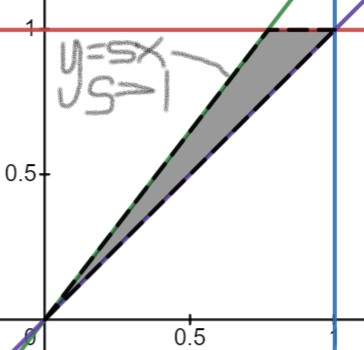
\includegraphics[scale=0.5]{3.1.2.1.jpg}
\caption{\(Y \leq sX\)}
\label{fig:3121}
%\addcontentsline{toc}{figure}{Figure \ref{fig:placeholder}} % Uncomment to add the figure to the table of contents
\end{figure}

\indent It follows that
\[
\Pr\left(\frac Y X \leq s\right) = \Pr(Y \leq sX) = 1 - \Pr(y > sX) = 1 - \int_0^{\frac{1}{s}}\int_{sx}^1 f(x, y)dydx = 1 - \frac{1}{s}.
\]
\indent Hence the cdf of \(S\) is
\[
F(s) = \left(1 - \frac{1}{s}\right)\mathbf{1}_{s \geq 1}, s \in \bR.
\]
\indent Differentiate with respect to \(s\) yields the pdf of \(S\):
\[
f(s) = \frac{1}{s^2}\mathbf{1}_{s \geq 1}.
\]
\end{example}

%----------------------------------------------------------------------------------------

\section{One-to-One Transformations}

\begin{definition} 
\index{One-to-one transformation}
\label{def:321}
Suppose \(X, Y\) are continuous rv's. A \textbf{one-to-one transformation} \(S\) of \(X\) and \(Y\) are two functions
\[
\begin{aligned}
U &= h_1(X, Y) \\
V &= h_2(X, Y)
\end{aligned}
\]
such that for all \((x, y)\) in the support of \((X, Y)\) (denoted \(R_{XY}\), \(h_1, h_2\) maps \((x, y)\) to \(R_{UV} \subseteq \bR^2\), the support for \((U, V)\).
\end{definition}

\begin{definition} \label{def:322}
\index{Jacobian matrix}
\index{Jacobian}
Suppose \(S:\bR^2\rightarrow\bR^2\) is defined by \(S(x, y) = (h_1(x, y), h_2(x, y)) = (u, v)\) for some \(h_1, h_2:\bR^2\rightarrow\bR\), then the \textbf{Jacobian matrix} of \(S\) is
\[
JS(x, y) = \begin{bmatrix}
\frac{\partial u}{\partial x} & \frac{\partial u}{\partial y} \\
\frac{\partial v}{\partial x} & \frac{\partial v}{\partial y}
\end{bmatrix}
\]
and the \textbf{Jacobian} of \(S\) is the determinant of the Jacobian matrix of \(S\):
\[
\frac{\partial(u, v)}{\partial(x, y)} = |JS(x, y)|.
\]
\end{definition}

\begin{theorem}[Inverse Mapping Theorem]
\label{thm:323}
\index{Inverse mapping theorem}
Let \(R \subseteq \bR^2\). Suppose \(S:R \rightarrow \bR^2\) defined by 
\[
S(x, y) = (h_1(x, y), h_2(x, y)) = (u, v)
\]
is a transformation such that \(\frac{\partial u}{\partial x}\), \(\frac{\partial u}{\partial y}\), \(\frac{\partial v}{\partial x}\), \(\frac{\partial v}{\partial y}\) are continuous functions and \(\frac{\partial(u, v)}{\partial(x, y)} \neq 0\) for all \((x, y) \in \bR\), then \(S\) is one-to-one on \(R\) and \(S^{-1}: \bR^2 \rightarrow R\) exists.
\end{theorem}
\begin{proof} We omit the proof. \end{proof}

\begin{remark} \label{rmk:324}
\hyperref[thm:323]{Thm. 3.2.3} provides a sufficient but not necessary condition for the existence of \(S^{-1}\). We now use this to give a formula for the pdf of a transformation of a 2-dimensional random vector using the Jacobian matrix of the transformation.
\end{remark}

\begin{theorem} \label{thm:325}
Let \(X, Y\) be continuous rv's with joint pdf \(f:\bR^2\rightarrow[0, 1]\) and support \(R_{XY} \subseteq \bR^2\). Suppose \(S\) is a one-to-one transformation
\[
\begin{aligned}
S: R_{XY} &\rightarrow R_{UV} \\
(x,y) &\mapsto (h_1(x, y), h_2(x, y)) 
\end{aligned}
\]
where \(h_1, h_2: \bR^2\rightarrow\bR\) are functions, \(R_{UV} \subseteq \bR^2\), with its inverse transformation
\[
\begin{aligned}
S^{-1}: R_{UV} &\rightarrow R_{XY} \\
(u, v) &\mapsto (w_1(u, v), w_2(u, v)),
\end{aligned}
\]
where \(w_1, w_2:\bR^2\rightarrow\bR\) are functions, then the pdf of \((U, V)\), \(g: R_{UV} \rightarrow [0, 1]\), is given by
\[
g(u, v) = f(w_1(u, v), w_2(u, v))\left|\frac{\partial(x, y)}{\partial(u, v)}\right| = f(w_1(u, v), w_2(u, v))\left|\left|\begin{smallmatrix} \frac{\partial x}{\partial u} & \frac{\partial x}{\partial v} \\
\frac{\partial y}{\partial u} & \frac{\partial y}{\partial v}
\end{smallmatrix}
\right|\right|.
\]
\end{theorem}
\begin{proof} Suppose \(S^{-1}\) maps from \(A \subseteq R_{UV}\) onto \(B \subseteq R_{XY}\), then
\[
\begin{aligned}
\Pr((U, V) \leq (u, v)) &= \iint_A g(u, v)dudv \\
&= \iint_B f(x, y)dxdy \\
&= \iint_A f(w_1(u, v), w_2(u, v))\left|\left|\begin{smallmatrix} \frac{\partial x}{\partial u} & \frac{\partial x}{\partial v} \\
\frac{\partial y}{\partial u} & \frac{\partial y}{\partial v}
\end{smallmatrix}
\right|\right|dudv
\end{aligned}
\]
where the last line follows from a theorem in calculus. Differentiate the above gives
\[
g(u, v) = f(w_1(u, v), w_2(u, v)) \left|\left|\begin{smallmatrix} \frac{\partial x}{\partial u} & \frac{\partial x}{\partial v} \\
\frac{\partial y}{\partial u} & \frac{\partial y}{\partial v}
\end{smallmatrix}
\right|\right|.
\]
\end{proof}

%----------------------------------------------------------------------------------------

\section{Moment Generating Function Technique}

\begin{theorem} \label{thm:331}
Suppose \(X_1, \ldots, X_n\) are independent rv's and each \(X_i\) has MGF \(M_i: (-h_i, h_i)\rightarrow\bR\), then the MGF of \(Y := \sum_{i=1}^n X_i\) is given by
\[
\begin{aligned}
M_Y: (-h, h) &\rightarrow \bR \\
t &\mapsto \prod_{i=1}^n M_i(t).
\end{aligned}
\]
\indent In particular, if the \(X_i\)'s have identical distributions, then \(Y\) has the MGF
\[
\begin{aligned}
M_Y: (-h, h) &\rightarrow \bR \\
t &\mapsto (M(t))^n.
\end{aligned}
\]
\end{theorem}
\begin{proof} By \hyperref[def:192]{the definition of MGFs}, we have
\[
\begin{aligned}
M_Y(t) &= E(e^{Yt}) \\
&= E\left(\exp\left(t\sum_{i=1}^n X_i\right)\right) \\
&= E\left(\exp\left(\sum_{i=1}^n tX_i\right)\right) \\
&= E\left(\prod_{i=1}^n \exp(tX_i)\right).
\end{aligned}
\]
\indent Since the \(X_i\)'s are independent, \(E\left(\prod_{i=1}^n \exp(tX_i)\right) = \prod_{i=1}^n E(tX_i)\), and hence
\[
M_Y(t) = \prod_{i=1}^n E(\exp(tX_i)) = \prod_{i=1}^n M_i(t)
\]
as required. \\
\indent If the \(X_i\)'s follow the same distribution, then all the \(M_i(t)\)'s are the same, and \(M_Y(t) = (M(t))^n\) immediately.
\end{proof}

\begin{theorem} \label{thm:332}
\index{Normal distribution!Sum of}
If \(X_i \sim N(\mu_i, \sigma_i^2)\) independently, \(1 \leq i \leq n\), then
\[
Y := \sum_{i=1}^n \alpha_iX_i \sim N\left(\sum_{i=1}^n \alpha_i\mu_i, \sum_{i=1}^n \alpha_i^2\sigma_i^2\right).
\]
\end{theorem}
\begin{proof} Using \hyperref[thm:331]{Thm. 3.3.1} and \hyperref[thm:197]{Thm. 1.9.7} we have
\[
M_Y(t) = \prod_{i=1}^n M_{\alpha_iX_i}(t) = \prod_{i=1}^n M_{X_i}(\alpha_i t)
\]
where each
\[
M_{X_i}(\alpha_i t) = \exp\left(\mu_i t + \sigma_i^2 + \frac{\alpha_i^2t^2}{2}\right).
\]
\indent Hence 
\[
M_Y(t) = \exp\left(\sum_{i=1}^n \alpha_i\mu_i t + \frac{\sigma_i^2\alpha_i^2 t^2}{2}\right) 
= \exp\left(t\sum_{i=1}^n \alpha_i\mu_i + \frac{t^2}{2} \sum_{i=1}^n \alpha_i^2\sigma_i^2\right), t \in \bR
\]
which is the MGF of
\[
N\left(\sum_{i=1}^n \alpha_i\mu_i, \sum_{i=1}^n\alpha_i^2 \sigma_i^2\right).
\]
\indent By the uniqueness of MGF's, this completes the proof.
\end{proof}

\begin{corollary} \label{cor:333}
\index{Normal distribution!Average of}
If each \(X_i \sim N(\sigma, \sigma^2)\) independently, \(1 \leq i \leq n\), then
\[
\sum_{i=1}^n X_i \sim N(n\mu, n\sigma^2)
\]
and
\[
\bar{X} = \frac{1}{n}\sum_{i=1}^n X_i \sim N\left(\mu, \frac{\sigma^2}{n}\right).
\]
\end{corollary}
\begin{proof} Take \hyperref[thm:332]{Thm. 3.3.2} and put each \(\alpha_i = 1\), \(\sigma_i = \sigma\), \(\mu_i = \mu\), and the result immediately follows. For the \(\bar{X}\) result, take \(\mu_i = \mu\), \(\sigma_i = \sigma\), and \(\alpha_i = \frac1n\).
\end{proof}

\begin{proposition} \label{prop:334}
\index{Chi-squared distribution!Sum of}
If \(X_i \sim \chi_{k_i}^2\) independently, \(1 \leq i \leq n\), then
\[
Y := \sum_{i=1}^n X_i \sim \chi^2_{\sum_{i=1}^n k_i}.
\]
\end{proposition}
\begin{proof} Each \(X_i\) has MGF
\[
M_i(t) = (1 - 2t)^{-k_i / 2}, t < \frac12.
\]
\indent By \hyperref[thm:331]{Thm. 3.3.1} we have
\[
M_Y(t) = \prod_{i=1}^n(1 - 2t)^{-k_i/2} = (1 - 2t)^{\sum_{i=1}^n \frac{-k_i}{2}} = (1 - 2t)^{-\frac{\sum_{i=1}^n k+i}{2}}, t < \frac12
\]
which is the MGF of
\[
\chi^2_{\sum_{i=1}^n k_i}.
\]
\indent By the uniqueness of MGF's, \(Y \sim \chi^2_{\sum_{i=1}^n k_i}\) as required.
\end{proof}

\begin{proposition} \label{prop:335}
\index{Normal distribution!Relationship with chi-squared distribution}
\index{Chi-squared distribution!Relationship with normal distribution}
If each \(X_i \sim N(\mu, \sigma^2)\) independently, \(1 \leq i \leq n\), then
\[
Y := \sum_{i=1}^n \left(\frac{X_i - \mu}{\sigma}\right)^2 \sim \chi^2_n.
\]
\end{proposition}
\begin{proof}
Denote, for each \(i\), \(Z_i = \frac{X_i - \mu}{\sigma}\), then each \(Z_i \sim N(0, 1)\). Define each \(U_i := Z_i^2\), then, if \(u_i \geq 0\),
\[
\begin{aligned}
\Pr(U_i \leq u_i) &= \Pr(Z_i^2 \leq u_i) \\
&= \Pr(-\sqrt{u_i} \leq Z_i \leq \sqrt{u_i}) \\
&= \int_{-\sqrt{u_i}}^{\sqrt{u_i}} \frac{1}{\sqrt{2\pi}}\exp\left(\frac{-z_i^2}{2}\right) dz_i \\
&= -\int_0^{-\sqrt{u_i}} \frac{1}{\sqrt{2\pi}}\exp\left(\frac{-z_i^2}{2}\right) dz_i + \int_0^{\sqrt{u_i}} \frac{1}{\sqrt{2\pi}} \exp\left(\frac{-z_i}{2}\right)dz_i.
\end{aligned}
\]
\indent Differentiate \(\Pr(U_i \leq u_i)\) with respect to \(u_i\) using the Fundamental Thm of Calculus to get the pdf of each \(U_i\) to be
\[
f(u_i) = -\frac{-1}{2\sqrt{u_i}}\frac{1}{\sqrt{2\pi}}\exp\left(\frac{-u_i}{2}\right) + \frac{1}{2\sqrt{u_i}}\frac{1}{\sqrt{2\pi}}\exp\left(\frac{-u_i}{2}\right) = \frac{1}{\sqrt{u_i}}\frac{1}{\sqrt{2\pi}}\exp\left(\frac{-u_i}{2}\right), u_i \geq 0.
\]
\indent By \hyperref[prop:146]{Proposition 1.4.6}, \(\sqrt{\pi} = \Gamma\left(\frac12\right)\), so re-write
\[
f(u_i) = \frac{u_i^{\frac12 - 1}e^{\frac{-u_i}{2}}}{2^{\frac12}\Gamma\left(\frac12\right)}, u_i \geq 0.
\]
\indent This shows that each
\[
\left(\frac{X_i - \mu}{\sigma}\right)^2 \sim \chi_1^2.
\]
\indent Using \hyperref[prop:334]{Proposition 3.3.4}, we have
\[
\sum_{i=1}^n\left(\frac{X_i - \mu}{\sigma}\right)^2 \sim \chi_n^2
\]
as required.
\end{proof}

\begin{remark} \label{rmk:336}
The next results illustrate techniques used in hypothesis testing. It starts out with a technique lemma and ends with a theorem concerning the student t-distribution.
\end{remark}

\begin{lemma} \label{lemma:337}
\index{\(S^2\)}
Suppose \(X_i \sim N(\mu, \sigma^2)\) independently, \(1 \leq i \leq n\). Define random variables
\[
\bar{X} = \frac1n\sum_{i=1}^n X_i, S^2 = \frac{\sum_{i=1}^n(X_i - \bar{X})^2}{n - 1},
\]
then \(\bar{X} \perp S^2\).
\end{lemma}
\begin{proof} For notational convenience, all \(\sum\) and \(\prod\) in this proof are over \(i\) from \(i = 1\) to \(i = n\).\\
\indent For each \(i\), define \(U_i := X_i - \bar{X}\), and \(U\) to be the random vector \(U := (U_1, \ldots, U_n)\). \\
\indent Write the joint MGF of \(U\) and \(\bar{X}\) to be
\[
M(s_1, \ldots, s_n, s) = E(\exp(\sum s_iU_i + s\bar{X})).
\]
Define \(t_i = s_i - \bar{s} + \frac{s}{n}\), where \(\bar{s} = \frac1n\sum s_i\). It follows that
\[
\begin{aligned}
&E(\exp(\sum t_iX_i)) \\
= &E\left(\exp\left(\sum s_iX_i - \sum \bar{s}X_i + \sum\frac{s}{n}X_i\right)\right) \\
= &E\left(\exp\left(\sum s_iX_i - \frac1n \sum s_iX_i + \frac{s}{n} \sum X_i\right)\right) \\
= &E\left(\exp\left(\sum s_i\left(X_i - \frac{X_i}{n}\right) + s\bar{X}\right)\right) \\
= &E\left(\exp\left(\sum s_i(X_i - \bar{X}) + s\bar{X}\right)\right) \\
= &E(\exp(\sum s_iU_i + s\bar{X})) \\
= &M(s_1, \ldots, s_n, s).
\end{aligned}
\]
\indent Hence, since each \(X_i \sim N(\mu, \sigma^2)\), 
\[
\begin{aligned}
M(s_1, \ldots, s_n, s) &= E(\exp(\sum t_iX_i)) \\
&= \prod E(\exp(t_iX_i)) \\
&= \prod \exp\left(\mu t_i + \frac{\sigma^2t_i^2}{2}\right) \\
&= \exp\left(\sum \left(\mu t_i + \frac{\sigma^2 t_i^2}{2}\right)\right).
\end{aligned}
\]
\indent Now \(\sum t_i = \sum\left(s_i - \bar{s} + \frac{s}{n}\right) = n\bar{s} - n\bar{s} + n\frac{s}{n} = s\), and
\[
\begin{aligned}
\sum t_i^2 &= \sum(s_i - \bar{s})^2 + 2\sum(s_i - \bar{s})\left(\frac{s}{n}\right) + \sum\left(\frac{s}{n}\right)^2 \\
&= \sum(s_i - \bar{s})^2 + \frac{1}{n^2}ns^2 \\
&= \sum(s_i - \bar{s})^2 + \frac{s^2}{n}
\end{aligned}
\]
which yields
\[
\begin{aligned}
M(s_1, \ldots, s_n, s) &= \exp\left(\mu\sum t_i + \frac{\sigma^2}{2}\sum t_i^2\right) \\
&= \exp\left(\mu s + \frac{\sigma^2}{2}\sum(s_i - \bar{s})^2 + \frac{\sigma^2}{2}\frac{s^2}{n}\right).
\end{aligned}
\]
\indent This means that the joint MGF of \(U_1, \ldots, U_n\) is
\[
M_U(s_1, \ldots, s_n) = M(s_1, \ldots, s_n, s=0) = \exp\left(\frac{\sigma^2}{2}\sum(s_i - \bar{s})^2\right)
\]
and the MGF of \(\bar{X}\) is
\[
M_{\bar{X}}(s) = M(s_1 = 0, \ldots, s_n = 0, s) = \exp\left(\mu s + \frac{\sigma^2s^2}{2n}\right).
\]
\indent Hence
\[
M(s_1, \ldots, s_n, s) = M_U(s_1, \ldots, s_n)M_{\bar{X}}(s)
\]
and so \(U \perp \bar{X}\) by \hyperref[thm:284]{Thm. 2.8.4}. By the definition of \(U\), each \(U_i = X_i - \bar{X}\) is independent of \(\bar{X}\), and consequently
\[
S^2 = \frac{(X_i - \bar{X})^2}{n - 1} \perp \bar{X}
\]
as required.
\end{proof}

\begin{proposition} \label{prop:338}
\index{Chi-squared distribution!Relationship with \(S^2\)}
If \(X_i \sim N(\mu, \sigma^2)\) independently, \(1 \leq i \leq n\), and we use the same rv \(S^2\) as in \hyperref[lemma:337]{Lemma 3.3.7}, then
\[
\frac{(n-1)S^2}{\sigma^2} = \frac{(n-1)\frac{\sum_{i=1}^n(X_i - \bar{X})^2}{n-1}}{\sigma^2} = \frac{\sum_{i=1}^n(X_i - \bar{X})^2}{\sigma^2} \sim \chi^2_{n-1}.
\]
\end{proposition}
\begin{proof} As before, all summations are over \(i\) from \(i = 1\) to \(i = n\). Recall that \(\bar{X} = \frac1n\sum X_i\). We have
\[
\begin{aligned}
\sum(X_i - \mu)^2 &= \sum(X_i - \bar{X} + \bar{X} - \mu)^2 \\
&= \sum(X_i - \bar{X})^2 + 2\sum(X_i - \bar{X})(\bar{X} - \mu) + \sum(\bar{X} - \mu)^2 \\
&= \sum(X_i - \bar{X})^2 + 0 - n(\bar{X} - \mu)^2 \\
&= \sum(X_i - \bar{X})^2 + n(\bar{X} - \mu)^2.
\end{aligned}
\]
\indent Hence
\[
\sum\left(\frac{X_i - \mu}{\sigma}\right)^2 = \frac{(n-1)S^2}{\sigma^2} + \left(\frac{\bar{X} - \mu}{\sigma / \sqrt{n}}\right)^2.
\]
\indent Denote \(Y := \sum\left(\frac{X_i - \mu}{\sigma}\right)^2\), \(U := \frac{(n - 1)S^2}{\sigma^2}\), \(V := \left(\frac{\bar{X} - \mu}{\sigma / \sqrt{n}}\right)^2\). \\
\indent Since \(S^2 \perp \bar{X}\) by \hyperref[lemma:337]{Lemma 3.3.7}, we have \(U \perp V\), and moreover by \hyperref[prop:335]{Proposition 3.3.5}, 
\[
Y = \sum\left(\frac{X_i - \mu}{\sigma}\right)^2 \sim \chi^2_n
\]
with MGF
\[
M_Y(t) = (1 - 2t)^{\frac{-n}{2}}, t < \frac12.
\]
\indent By \hyperref[cor:333]{Corollary 3.3.3}, 
\[
\bar{X} \sim N\left(\mu, \frac{\sigma^2}{n}\right),
\]
and so
\[
\frac{\bar{X} - \mu}{\sigma / \sqrt{n}} \sim N(0, 1).
\]
\indent By \hyperref[prop:335]{Proposition 3.3.5} again, 
\[
V = \left(\frac{\bar{X} - \mu}{\sigma / \sqrt{n}}\right)^2 \sim \chi_1^2
\]
with MGF
\[
M_V(t) = (1 - 2t)^{-\frac12}, t < \frac12.
\]
\indent Now \(Y = U + V\) and \(U \perp V\), so
\[
M_Y(t) = M_U(t)M_V(t)
\]
which gives
\[
M_U(t) = E(e^{tU}) = \frac{M_Y(t)}{M_V(t)} = \frac{(1 - 2t)^{-\frac{n}{2}}}{(1 - 2t)^{-\frac12}} = (1 - 2t)^{-\frac{n-1}{2}}, t < \frac12.
\]
\indent This is the MGF of \(\chi^2_{n-1}\). By the uniqueness of MGF's, \(\frac{(n-1)S^2}{\sigma^2} = U \sim \chi^2_{n-1}\) as required. 
\end{proof}

\begin{lemma} \label{lemma:339}
\index{Student \(t\)-distribution}
\index{Student \(t\)-distribution!Relationship with normal distribution}
If \(X \sim \chi^2_n\), \(Z \sim N(0, 1)\), and \(X \perp Z\), then
\[
T := \frac{Z}{\sqrt{X / n}} \sim t_n
\]
where \(t_n\) is the student \(t\)-distribution with \(n\) degrees of freedom.
\end{lemma}
\begin{proof}
Define a one-to-one transformation \(S:\bR^2 \rightarrow\bR^2\):
\[
S(Z, X) = (T, U) = \left(\frac{Z}{\sqrt{X / n}}, X\right).
\]
\indent \(S\) has the reverse transformation
\[
S^{-1}(T, U) = (Z, X) = \left(T\left(\frac{U}{n}\right)^{\frac12}, U\right).
\]
\indent Since \(X \sim \chi^2_n\), \(Z \sim N(0, 1)\) and \(X \perp Z\), the joint pdf of \((Z, X)\) is the product of the marginal pdf's, namely
\[
f_{ZX}(z, x) = f_Z(z)f_X(x) = \frac{e^{-z^2/2}}{\sqrt{2\pi}}\cdot\frac{x^{\frac{n}{2}-1}e^{-\frac{x}{2}}}{2^{\frac{n}{2}}\Gamma\left(\frac{n}{2}\right)}, x > 0, z \in \bR.
\]
\indent Using \hyperref[thm:325]{Thm. 3.2.5}, the joint pdf of \((T, U)\) is
\[
\begin{aligned}
g(t, u) &= f\left(t\left(\frac{u}{n}\right)^{\frac12}, u\right)\left|\frac{\partial(z, x)}{\partial(t, u)}\right| \\
&= \frac{e^{-\frac{t^2u}{2n}}}{\sqrt{2\pi}}\cdot\frac{u^{\frac{n}{2}-1}e^{-\frac{u}{2}}}{2^{\frac{n}{2}}\Gamma\left(\frac{n}{2}\right)}\left|\left|\begin{smallmatrix} \frac{\partial z}{\partial t} & \frac{\partial z}{\partial u} \\
\frac{\partial x}{\partial t} & \frac{\partial x}{\partial u}\end{smallmatrix}\right|\right| \\
&= \frac{e^{-\frac{t^2u}{2n}}}{\sqrt{2\pi}}\cdot\frac{u^{\frac{n}{2}-1}e^{-\frac{u}{2}}}{2^{\frac{n}{2}}\Gamma\left(\frac{n}{2}\right)}\left|\left|\begin{smallmatrix} \left(\frac{u}{n}\right)^{\frac12} & 0 \\
0 & 1\end{smallmatrix}\right|\right| \\
&= \frac{e^{-\frac{t^2u}{2n}}}{\sqrt{2\pi}}\cdot\frac{u^{\frac{n}{2}-1}e^{-\frac{u}{2}}}{2^{\frac{n}{2}}\Gamma\left(\frac{n}{2}\right)}\left(\frac{u}{n}\right)^{\frac12}, t \in \bR, u > 0.
\end{aligned}
\]
\indent From this we get the marginal pdf of \(T\):
\[
f_T(t) = \int_{-\infty}^\infty g(t, u)du.
\]
\indent This eventually yields
\[
f_T(t) = \frac{\Gamma\left(\frac{n+1}{2}\right)}{\Gamma\left(\frac{n}{2}\right)\sqrt{\pi n}} \left(1 + \frac{t^2}{2}\right)^{-\frac{n+1}{2}}, t \in bR,
\]
which is exactly the pdf of the Student \(t\)-distribution of \(n\) degrees of freedom, so \(T \sim t_n\) as required.\\
\indent The trick with the integration above is to let
\[
y = u\left(\frac12 + \frac{t^2}{2n}\right)
\]
and substitute \(u\) and \(du\) in terms of \(y\) and \(dy\).
\end{proof}

\begin{theorem} \label{thm:3310}
\index{\(S^2\)!Relationship with student \(t\)-distribution}
If \(X_i \sim N(\mu, \sigma^2)\) independently, \(1 \leq i \leq n\), then
\[
\frac{\bar{X} - \mu}{S / \sqrt{n}} \sim t_{n-1}
\]
where
\[
S = \sqrt{\frac{\sum_{i=1}^n (X_i - \bar{X})^2}{n-1}}.
\]
\end{theorem}
\begin{proof} Re-write
\[
\begin{aligned}
\frac{\bar{X} - \mu}{S / \sqrt{n}} &= \frac{\bar{X} - \mu}{S / \sqrt{n}} \cdot \frac{\sigma/\sqrt{n}}{\sigma/\sqrt{n}} \\
&= \frac{\frac{\bar{X} - \mu}{\sigma/\sqrt{n}}}{\frac{S}{\sqrt{n}}\cdot\frac{\sqrt{n}}{\sigma}} \\
&= \frac{\frac{\bar{X} - \mu}{\sigma / \sqrt{n}}}{\frac{S(n-1)/\sigma}{n-1}} \\
&= \frac{\frac{\bar{X} - \mu}{\sigma / \sqrt{n}}}{\sqrt{\frac{S^2(n-1)/\sigma^2}{n-1}}}
\end{aligned}
\]
where \(\frac{\bar{X} - \mu}{\sigma/\sqrt{n}} \perp \frac{S^2(n-1)}{\sigma^2}\) by \hyperref[prop:338]{Proposition 3.3.8}. Furthermore
\[
\frac{\bar{X} - \mu}{\sigma/\sqrt{n}} \sim N(0, 1)
\]
by \hyperref[cor:333]{Corollary 3.3.3} and
\[
\frac{S^2(n-1)}{\sigma^2} \sim \chi^2_{n-1}
\]
by \hyperref[prop:338]{Proposition 3.3.8}. Apply \hyperref[lemma:339]{Lemma 3.3.9} to get
\[
\frac{\bar{X} - \mu}{S / \sqrt{n}} \sim t_{n-1}
\]
as required.
\end{proof}

\begin{remark} \label{rmk:3311}
\index{Sample variance}
\index{Sample standard deviation}
\(S^2\) in \hyperref[prop:338]{Proposition 3.3.8} and \hyperref[thm:3310]{Thm. 3.3.10} is the \textbf{sample variance} of a random sample \(X_1, \ldots, X_n\), while \(S\) is the \textbf{sample standard deviation}. \hyperref[prop:338]{Proposition 3.3.8} and \hyperref[thm:3310]{Thm. 3.3.10} are useful when constructing estimates and confidence intervals for the \(\sigma^2\) parameter given a random sample with assumed underlying distribution of \(N(\mu, \sigma^2)\).
\end{remark}


%----------------------------------------------------------------------------------------
%	CHAPTER 4
%----------------------------------------------------------------------------------------

\chapterimage{chapter_head_1.pdf} % Chapter heading image

\chapter{Limiting Asymptotic Distributions}

%----------------------------------------------------------------------------------------

\section{Convergence in Distribution}

\begin{definition} \label{def:411}
\index{Convergence!In Distribution}
Let \((X_n)_{n=1}^\infty\) be a sequence of rv's and \((F_n(x))_{n=1}^\infty\) be the corresponding cdf's. Let \(X\) be a rv with cdf \(F\). We say that \((X_n)_n\) \textbf{converges in distribution} to \(X\) and write
\[
X_n\xrightarrow{D} X
\]
if \(\lim_{n\rightarrow\infty}F_n(x) = F(x)\) pointwise for all \(x \in \bR\) at which \(F\) is continuous.
\end{definition}

\begin{remark} \label{rmk:412}
We state some facts from real analysis that helps with finding limiting distributions.
\begin{enumerate}
\item Suppose \(a < b\) and \(f:[a, b]\rightarrow\bR\) is in \(C^\infty\), i.e. infinitely differentiable and all derivatives are continuous on \([a, b]\). Let \(c \in [a, b]\), then for all \(x \in [a, b]\) and \(k \in \bN\), we have
\[
f(x) = \sum_{i=0}^k \frac{f^{(i)}(c)(x-c)^i}{i!} + \frac{f^{(k+1)}(\xi_x)(x - c)^{k + 1}}{(k+1)!}
\]
for some \(\xi_x \in [x, c]\) or \([c, x]\).
\item Let \(b, c \in \bR\), \(\Phi\) a function from \(\bR\) to \(\bR\) with \(\lim_{n\rightarrow\infty} \Phi(n) = 0\), then
\[
\lim_{n\rightarrow\infty}\left(1 + \frac{b}{n} + \frac{\Phi(n)}{n}\right)^{cn} = e^{bc}.
\]
\begin{proof}
Consider the Taylor expansion of \(\log(1 + x)\) about \(c = 0\):
\[
\begin{aligned}
\log(1+x) &= \sum_{i=0}^1 \frac{f^{(i)}(0)(x-0)^i}{i!} + \frac{f^{(2)}(\xi_x)(x-0)^2}{2!} \\
&= \frac{\log(1)x^0}{0!} + \frac{\frac{1}{1+0}(x-0)^i}{1!} + \frac{\frac{-1}{(1 - \xi_x)^2}x^2}{2!} \\
&= x - \frac{x^2}{2(1 + \xi_x)^2}, \xi_x \in [0, x].
\end{aligned}
\]
\indent Therefore
\[
\log\left(1 + \frac{b}{n} + \frac{\Phi(n)}{n}\right) = \frac{b}{n} + \frac{\Phi(n)}{n} - \frac{\left(\frac{b}{n} + \frac{\Phi(n)}{n}\right)^2}{2(1 + \xi_x)^2}
\]
and
\[
cn\cdot\log\left(1 + \frac{b}{n} + \frac{\Phi(n)}{n}\right) = bc + \Phi(n)c - \frac{(b + \Phi(n))^2}{2n(1 + \xi_x)^2}
\]
which yields
\[
\lim_{n\rightarrow\infty} cn\cdot\log\left(1 + \frac{b}{n} + \frac{\Phi(n)}{n}\right) = bc
\]
as required.
\end{proof}
\item Let \(b, c \in \bR\), then
\[
\lim_{n\rightarrow\infty}\left(1 + \frac{b}{n}\right)^{cn} = e^{bc}.
\]
\end{enumerate}
\end{remark}

\begin{example} \label{eg:413}
Consider a sequence \((X_i)_i\) where each
\[
X_i \sim \unifDist\left(0, \frac{1}{i}\right),
\]
and denote the cdf of \(X_i\) to be \(F_i\).\\
\indent Define \(X\) such that \(\Pr(X = 0) = 1\). Consider the cdf \(F_X: \bR\rightarrow[0, 1]\) of \(X\). Clearly \(F_X(x) = \mathbf{1}_{x \geq 0}\). In particular \(F_X\) has a jump discontinuity at \(x = 0\). \\
\indent Fix \(x \neq 0\). \\
\indent If \(x < 0\), then each \(0 \leq F_i(x) = \Pr(X_i \leq x) \leq \Pr(X_i < 0) = 0\), so \(F_i(x) = 0\). \\
\indent For each \(i \in \bN\), if \(x \in \left[0, \frac1i\right]\), then \(F_i(x) = \int_0^x 1/(1/i)dx = ix\). If \(x > \frac1i\), \(F_i(x) = 1\). \\
\indent In summary
\[
F_i(x) = \Pr(X_i \leq x) = \left\{
\begin{array}{rcl}
0 & \IF & x < 0 \\
ix & \IF & x \in \left[0, \frac1i\right] \\
1 & \IF & x > \frac1i
\end{array}
\right.
\]
\indent As \(i\rightarrow\infty\), \(\frac1i \rightarrow 0\). Now note that the cdf of \(X\) is
\[
F_X(x) = \left\{
\begin{array}{rcl}
0 & \IF & x < 0 \\
1 & \IF & x \geq 0
\end{array}
\right.
\]
\indent Thus for every \(x \neq 0\), \(F_i(x)\rightarrow F(x)\) pointwise as \(i \rightarrow \infty\). Thus \(X_i \xrightarrow{D} X\) by definition. \\
\indent This naturally gives rise to the following definition.
\end{example}

\begin{definition} \label{def:414}
\index{Degenerate distribution}
Fix \(c \in \bR\). A rv \(Y\) has a \textbf{degenerate distribution} at \(y = c\) if \(Y\) has the cdf
\[
F_Y(y) = \mathbf{1}_{y \geq c}, y \in \bR,
\]
i.e. \(Y\) has pdf \(f_Y(y) = \mathbf{1}_{y = c}, y \in \bR\).
\end{definition}

\begin{definition} \label{def:415}
\index{Convergence!Stochastically}
\((X_i)_i\) is said to \textbf{converge stochastically to a constant} \(c\) if \(X_i \xrightarrow{D} X\), where \(X\) is a degenerate distribution at \(c\).
\end{definition}

%----------------------------------------------------------------------------------------

\section{Convergence in Probability}

\begin{definition} \label{def:421}
\index{Convergence!In probability}
A sequence of rv's \((X_n)_{n=1}^\infty\) \textbf{converges in probability} to a random variable \(X\) if for all \(\ep > 0\),
\[
\lim_{n\rightarrow\infty} \Pr(|X_n - X| \geq \ep)= 0,
\]
or equivalently
\[
\lim_{n\rightarrow\infty} \Pr(|X_n - X| < \ep) = 1.
\]
\indent We write \(X_n \xrightarrow{P}X\).
\end{definition}

\begin{theorem} \label{thm:422}
Let \((X_n)_n\) be a sequence of rv's. If \(X_n \xrightarrow{P}X\) for some rv \(X\), then \(X_n\xrightarrow{D}X\).
\end{theorem}
\begin{proof}
Suppose that \(X_n \xrightarrow{P}X\). We show that for all \(\ep > 0\),
\[
F_X(a - \ep) \leq \lim_{n\rightarrow\infty}F_n(a) \leq F_X(a + \ep)
\]
for all \(a \in \bR\) such that \(F_X\) is continuous at \(a\). This directly implies the result we need.\\
\indent Fix \(a \in \bR\) such that \(F_X\) is continuous at \(a\). Denote \(F_n\) to be the cdf of \(X_n\). Note that for each \(n \in \bN\), 
\[
\begin{aligned}
F_n(a) &= \Pr(X_n \leq a, X \leq a + \ep) + \Pr(X_n \leq a, X > a + \ep) \\
&= \Pr(X_n \leq a | X \leq a + \ep)\Pr(X \leq a + \ep) + \Pr(X_n \leq a, X > a + \ep) \\
&\leq \Pr(X \leq a + \ep) + \Pr(X_n \leq a, X > a + \ep) \\
&= \Pr(X \leq a + \ep) + \Pr(X_n \leq a, X - \ep > a) \\
&\leq \Pr(X \leq a + \ep) + \Pr(X - \ep > X_n) \SINCE a \geq X_n \\
&\leq \Pr(X \leq a + \ep) + \Pr(X_n - X < -\ep) + \Pr(X_n - X > \ep) \\
&= \Pr(X \leq a + \ep) + \Pr(|X_n - X| > \ep).
\end{aligned}
\]
\indent Thus 
\begin{equation} \label{eqn:4221}
\Pr(X \leq a + \ep) \geq F_n(a) - \Pr(|X_n - X| > \ep).
\end{equation}
\indent Similarly, 
\[
\begin{aligned}
F_X(a - \ep) &= \Pr(X \leq a - \ep) \\
&= \Pr(X \leq a - \ep, X_n \leq a) + \Pr(X \leq a - \ep, X_n > a) \\
&\leq \Pr(X \leq a - \ep|X_n\leq a)\Pr(X_n \leq a) + \Pr(X \leq a - \ep, X_n > a) \\
&\leq \Pr(X_n \leq a) + \Pr(X + \ep \leq a, a < X_n) \\
&\leq \Pr(X_n \leq a) + \Pr(X + \ep < X_n) \\
&\leq \Pr(X_n \leq a) + \Pr(X - X_n > \ep) + \Pr(X - X_n < -\ep) \\
&= \Pr(X_n \leq a) + \Pr(|X - X_n| > \ep)
\end{aligned}
\]
which shows that
\begin{equation} \label{eqn:4222}
F_X(a - \ep) \leq F_n(a) - \Pr(|X_n - X| > \ep).
\end{equation}
\indent By \hyperref[def:421]{Def. 4.2.1}, for a \(\ep > 0\), \(\Pr(|X_n - X| > \ep)\) can be made arbitrarily small. Hence, as \(n\rightarrow\infty\), \hyperref[eqn:4221]{(4.1)} becomes 
\[
\begin{aligned}
&\lim_{n\rightarrow\infty} F_n(a) - \Pr(|X_n - X| > \ep) \\
= &\lim_{n\rightarrow\infty} F_n(a) - \lim_{n\rightarrow\infty}\Pr(|X_n - X| > \ep) \\
= &\lim_{n\rightarrow\infty} F_n(a) 
\leq \Pr(X \leq a + \ep) 
= F_X(a + \ep).
\end{aligned}
\]
\indent Similarly inequality \hyperref[eqn:4222]{(4.2)} yields
\[
\lim_{n\rightarrow\infty} F_n(a) \geq F_X(a - \ep),
\]
which, together, yields the desired result:
\[
F_X(a - \ep) \leq \lim_{n\rightarrow\infty}F_n(a) \leq F_X(a + \ep).
\]
\indent This completes the proof.
\end{proof}

\begin{theorem} \label{thm:423}
The sequence \((X_n)_n\) converges stochastically to a constant \(c\) if and only if \((X_n)_n\) converges in probability to the degenerate distribution at \(c\), i.e. for all \(\ep > 0\),
\[
\lim_{n\rightarrow\infty}\Pr(|X_n - c| < \ep) = 1.
\]
\end{theorem}
\begin{proof} \((\Rightarrow)\) Suppose \(X_n \xrightarrow{D}X\) where \(X\) is the degenerate distribution at \(c\), then the pointwise limit of \(F_n(x)\), which are the cdf's of \(X_n\)'s, is \(F(x) = \mathbf{1}_{x \geq c}\). \\
\indent Let \(\ep > 0\), then
\[
\begin{aligned}
\Pr(|X_n - c| < \ep) &= \Pr(X_n - c < \ep) + \Pr(X_n - c > -\ep) \\
&= \Pr(X_n < \ep + c) + \Pr(X_n > c - \ep) \\
&= \Pr(X_n < \ep + c) + 1 - \Pr(X_n \leq c - \ep).
\end{aligned}
\]
\indent Take \(n\rightarrow\infty\), then \(\Pr(X_n < \ep + c)\) converges to \(\Pr(X < \ep + c)\) and \(\Pr(X_n \leq c - \ep)\) converges to \(\Pr(X \leq c - \ep)\) by the pointwise convergence of \(F_n\) to \(F_X\). Since \(c - \ep < c\), we have
\[
\Pr(X_n \leq c - \ep) \rightarrow 0.
\]
\indent Moreover, since \(\ep > 0\) is arbitrary,
\[
\Pr(X_n < c + \ep) \rightarrow 0.
\]
\indent So \(\Pr(|X_n - c| < \ep) \rightarrow 1\) and this completes the proof. \\
\((\Leftarrow)\) Suppose conversely that \(X_n\xrightarrow{P}X\) where \(X\) is a degenerate distribution at \(c\). Apply \hyperref[thm:422]{Thm. 4.2.2} directly and we get \(X_n \xrightarrow{D} X\) as required.
\end{proof}

\begin{remark} \label{rmk:424}
For a constant \(c\), we observe that
\[
\begin{aligned}
& X_n \xrightarrow{P} c \\
\Leftrightarrow &X_n \xrightarrow{D} c \\
\Leftrightarrow &\lim_{n\rightarrow\infty}\Pr(|X_n - c| \geq \ep) = 0 \\
\Leftrightarrow &\lim_{n\rightarrow\infty}\Pr(|X_n - c| < \ep) = 1.
\end{aligned}
\]
\end{remark}

%----------------------------------------------------------------------------------------

\section{Weak Law of Large Numbers}

\begin{theorem}[Weak Law of Large Numbers]
\index{Weak law of large numbers}
\label{thm:431}
Suppose \((X_n)_n\) are independently and identically distributed with each \(E(X_i) = \mu\) and \(\var(X_i) = \sigma^2\). Define the sequence \((\bar{X}_n)_n\) where each
\[
\bar{X}_n = \frac1n\sum_{i=1}^nX_i.
\]
\indent Then \(\bar{X}_n\xrightarrow{P}\mu\).
\end{theorem}
\begin{proof} Let \(\ep > 0\).\\
\indent By construction, each \(\var(\bar{X}_n) = \frac{\sigma^2}{n}\). Denote \(\sigma_n = \frac{\sigma}{\sqrt{n}}\), then let \(k_n = \frac{\ep}{\sigma_n}\). By \hyperref[cor:184]{Chebyshev's Inequality}, 
\[
\Pr(|\bar{X}_n - \mu| \geq k_n\sigma_n) = \Pr\left(|\bar{X}_n - \mu| \geq \frac{\ep}{\sigma_n}\sigma_n\right) \leq k_n^2 = \frac{\sigma_n^2}{\ep^2}.
\]
\indent Thus
\[
\Pr(|\bar{X}_n - \mu| \geq \ep) \leq \frac{\sigma^2}{n\ep^2} \SINCE \sigma_n^2 = \frac{\sigma^2}{n}
\]
and
\[
0 \leq \lim_{n\rightarrow\infty}\Pr(|\bar{X}_n - \mu|\geq\ep) \leq \lim_{n\rightarrow\infty}\frac{\sigma^2}{n\ep^2} = 0
\]
giving, by the Squeeze Theorem,
\[
\lim_{n\rightarrow\infty}\Pr(|\bar{X}_n - \mu|\geq\ep) = 0.
\]
\indent By definition, \(\bar{X}_n\xrightarrow{P}\mu\).
\end{proof}

%----------------------------------------------------------------------------------------

\section{MGF Technique for Limiting Distributions}

\begin{theorem} \label{thm:441}
Let \((X_n)_n\) be a sequence of rv's with MGF's \((M_n(t))_n\). Suppose \(X\) is a rv with MGF \(M(t)\). If there exists \(h > 0\) such that
\[
\lim_{n\rightarrow\infty}M_n(t) = M(t)
\]
for all \(t \in (-h, h)\), then
\[
X_n\xrightarrow{D}X.
\]
\end{theorem}
\begin{proof}
We omit the proof.
\end{proof}

\begin{remark} \label{rmk:442}
We next prove the Central Limit Theorem using the above result. It is not the most robust proof because it assumes that each rv in the sequence has a well-defined MGF.
\end{remark}

\begin{theorem}[Central Limit Theorem]
\label{thm:443}
\index{Central limit theorem}
Let \((X_i)_i\) be a sequence of independently, identically distributed rv's with each \(E(X_i) = \mu\), \(\var(X_i) = \sigma^2\) which are both finite, then
\[
\frac{n\bar{X} - n\mu}{\sqrt{n}\sigma} = \frac{\bar{X} - \mu}{\sigma/\sqrt{n}} = \frac{\sqrt{n}(\bar{X} - \mu)}{\sigma} \xrightarrow{D} Z \sim N(0, 1)
\]
where \(\bar{X} = \frac1n\sum_{i=1}^n X_i\).
\end{theorem}
\begin{proof}
Since all \(X_i\)'s have a well-defined MGF, let \(m_i: (-h_i. h_i)\rightarrow\bR\) be the MGF of \(X_i - \mu\). By \hyperref[rmk:193]{Remark 1.9.3} and \hyperref[prop:194]{Proposition 1.9.4}, for each \(i\),
\[
\begin{aligned}
m_i(0) &= 1 \\
m_i'(0) &= E(X_i - \mu) = 0 \\
m_i''(0) &= E((X_i - \mu)^2) = \sigma^2.
\end{aligned}
\]
\indent Now, for \(t \in (-h_i, h_i)\), the MacLaurin series of \(m_i(t)\) is
\[
m_i(t) = m(0) + m'(0)t + \frac{m''(\xi)t^2}{2!}
\]
for some \(\xi \in [0, t]\) or \(\xi \in [t, 0]\). Re-write:
\[
m_i(t) = 1 + \frac{m''(\xi)t^2}{2} + \frac{\sigma^2t^2}{2} - \frac{\sigma^2t^2}{2} = 1 + \frac{\sigma^2t^2}{2} + \frac{m''(\xi) - \sigma^2}{2}t^2.
\]
\indent Now define
\[
Z_n = \frac{\bar{X} - \mu}{\sigma / \sqrt{n}} = \frac{n\bar{X} - n\mu}{\sqrt{n}\sigma} = \frac{n(\sum_{i=1}^n X_i / n) - \sum_{i=1}^n \mu}{\sqrt{n}\sigma} = \frac{\sum_{i=1}^n(X_i - \mu)}{\sqrt{n}\sigma}.
\]
\indent Hence the MGF of \(Z\), by \hyperref[thm:197]{Thm. 1.9.7} and \hyperref[thm:331]{Thm. 3.3.1}, is
\[
\begin{aligned}
M_{Z_n}(t) &= \prod_{i=1}^n m_i\left(\frac{t}{\sqrt{n}\sigma}\right) \\
&= \left(1 + \frac{\sigma^2\left(\frac{t}{\sqrt{n}\sigma}\right)^2}{2} + \frac{m''(\xi) - \sigma^2}{2}\left(\frac{t}{\sqrt{n}\sigma}\right)^2\right)^n \\
&= \left(1 + \frac{t^2}{2n} + \frac{m''(\xi) - \sigma^2}{2n\sigma^2}t^2\right)^n, |\xi| < \left|\frac{t}{\sqrt{n}\sigma}\right| \\
&= \left(1 + \frac{t^2}{2n} + \frac{(m''(\xi) - \sigma^2)t^2 / 2\sigma^2}{n}\right)^n, |\xi| < \left|\frac{t}{\sqrt{n}\sigma}\right|.
\end{aligned}
\]
\indent As \(n\rightarrow\infty\), \(\left|\frac{t}{\sqrt{n}\sigma}\right| \rightarrow 0\), and thus \(\xi\rightarrow 0\). This means that as \(n\rightarrow\infty\), 
\[
m''(\xi)\rightarrow m''(0) = \sigma^2 \quad (m'' \text{ continuous})
\]
and consequently as \(n\rightarrow\infty\),
\[
(m''(\xi) - \sigma^2)t^2/2\sigma^2 \rightarrow 0.
\]
\indent By \hyperref[rmk:412]{Remark 4.1.2}(2),
\[
\lim_{n\rightarrow\infty}M_{Z_n}(t) = \lim_{n\rightarrow\infty}\left(1 + \frac{t^2}{2n} + \frac{(m''(\xi) - \sigma^2)t^2 / 2\sigma^2}{n}\right)^n = e^{\frac{t^2}{2}}, t \in \bR.
\]
\indent Thus by \hyperref[thm:441]{Thm. 4.4.1}, \(Z_n \xrightarrow{D} Z \sim N(0, 1)\) since \(e^{\frac{t^2}{2}}, t \in \bR\) is the MGF of \(N(0, 1)\).
\end{proof}

\begin{remark} \label{rmk:444}
Below we present several small results, which lead to the so-called \(\delta\)-method, which helps determine the limiting distribution of a function of a sequence of rv's. The function needs to have some nice properties.
\end{remark}

\begin{proposition} \label{prop:445}
If \(X_n\xrightarrow{P} a\) for some \(a \in \bR\), i.e. \(X_n\xrightarrow{P}X\) where \(X\) is a degenerate distribution at \(a\), and \(g:\bR\rightarrow\bR\) is a continuous function at \(a\), then \(g(X_n) \xrightarrow{P} g(a)\).
\end{proposition}
\begin{proof}
Let \(\ep > 0\). Because \(g\) is continuous at \(a\), there exists \(\delta > 0\) such that \(|x - a| < \delta\) implies \(|g(x) - g(a)| < \ep\). This further implies that the event \((|X - a| < \delta) \subseteq (|g(X_n) - g(a)| < \ep\) for each \(n\). Therefore
\[
\Pr(|g(X_n) - g(a)| < \ep) \geq \Pr(|X - a| < \delta)
\]
and taking limit yields
\[
\lim_{n\rightarrow\infty}\Pr(|g(X_n) - g(a)| < \ep) \geq \lim_{n\rightarrow\infty} \Pr(|X - a| < \delta).
\]
\indent Now \(X_n \xrightarrow{P} X\), so by definition
\[
\lim_{n\rightarrow\infty}\Pr(|g(X_n) - g(a)| < \ep) \geq \lim_{n\rightarrow\infty} \Pr(|X - a| < \delta) = 1.
\]
\indent But of course, all probabilities are \(\leq 1\), so
\[
\lim_{n\rightarrow\infty}\Pr(|g(X_n) - g(a) < \ep) \leq 1.
\]
\indent In summary,
\[
\lim_{n\rightarrow\infty}\Pr(|g(X_n) - g(a) < \ep) \leq 1 \leq \lim_{n\rightarrow\infty}\Pr(|g(X_n) - g(a) < \ep).
\]
\indent The Squeeze Theorem yields
\[
\lim_{n\rightarrow\infty}\Pr(|g(X_n) - g(a) < \ep) = 1
\]
and so \(g(X_n) \xrightarrow{P} g(a)\).
\end{proof}

\begin{proposition} \label{prop:446}
If \(X_n\xrightarrow{P} a\), \(Y_n \xrightarrow{P} b\), \(a, b \in \bR\), and \(g:\bR^2\rightarrow\bR\) is continuous at \((a, b)\), then
\[
g(X_n, Y_n) \xrightarrow{P} g(a, b).
\]
\end{proposition}
\begin{proof} We omit the proof.\end{proof}

\begin{theorem}[Slutsky's Theorem]
\label{thm:447}
\index{Slutsky's theorem}
If \(X_n\xrightarrow{P} c\) for some \(c \in \bR\) and \(Y_n \xrightarrow{P} Y\), then
\begin{enumerate}
\item \(X_n + Y_n \xrightarrow{D} c + Y\).
\item \(X_nY_n \xrightarrow{D} cY\).
\item \(\frac{Y_n}{c} \xrightarrow{D} \frac{Y}{c}\) if \(c \neq 0\).
\end{enumerate}
\end{theorem}
\begin{proof} We omit the proof.\end{proof}

\begin{theorem}[The \(\delta\)-method]
\label{thm:448}
\index{\(\delta\)-method}
Suppose \((X_i)_i\) is a sequence of rv's with
\[
n^b(X_i - a) \xrightarrow{D} X
\]
for some \(b > 0\), \(a \in \bR\). Suppose \(g:\bR\rightarrow\bR\) is a function such that \(g\) is differentiable at \(a\) with \(g'(a) \neq 0\), then
\[
n^b(g(X_i) - g(a)) \xrightarrow{D} g'(a)X.
\]
\end{theorem}
\begin{proof}
Since \(b > 0\), we have \(\lim_{n\rightarrow\infty} n^{-b} = 0\) and hence
\[
\lim_{n\rightarrow\infty}\Pr(|n^{-b} - 0| \geq \ep) = 0
\]
i.e. \(n^{-b} \xrightarrow{P} 0\).\\
\indent Since \(n^b(X_i - a)\xrightarrow{D} X\) and \(n^{-b} \xrightarrow{P}0\), by \hyperref[thm:447]{Slutsky's Theorem},
\[
X_i - a = n^{-b}n^b(X_i - a) \xrightarrow{D} 0.
\]
\indent Now, by \hyperref[thm:423]{Thm. 4.2.3}, we have \(X_i - a \xrightarrow{P} 0\). Use Taylor expansion of \(g(X_i)\) around \(a\) to yield
\[
g(X_i) = g(a) + \frac{g'(\xi)(X_i - a)}{1!}
\]
for some \(\xi \in [a, X_i]\) or \(\xi \in [X_i, a]\).\\
\indent Since \(X_i \xrightarrow{P}a\) as \(i\rightarrow\infty\), \(\xi\rightarrow a\) and hence \(\xi \xrightarrow{P}a\). But \(g'\) is continuous at \(a\), so
\[
g'(\xi) \xrightarrow{P} g'(a).
\]
\indent In combination with the fact that \(n^b(X_i - a)\xrightarrow{D}X\), use \hyperref[thm:447]{Slutsky's Theorem} again to yield
\[
g'(\xi)n^b(X_i - a) \xrightarrow{D} g'(a)X.
\]
\indent However \(g'(\xi)(X_i - a) = g(X_i) - g(a)\). Substitution yields
\[
n^b(g(X_i) - g(a)) \xrightarrow{D} g'(a)X
\]
as required.
\end{proof}

\begin{corollary} \label{cor:449}
If \((X_i)_i\) is a sequence of rv's with \(E(X_i) = \mu\) and \(\var(X_i) = \sigma^2\), and \(g:\bR\rightarrow\bR\) is differentiable at \(\mu\) with \(g'(\mu) \neq 0\), then
\[
\sqrt{n}(g(\bar{X}_n) - g(\mu)) \xrightarrow{D} X \sim N(0, (g'(\mu))^2\sigma^2).
\]
\end{corollary}
\begin{proof} By \hyperref[thm:443]{the Central Limit Theorem} we have
\[
\sqrt{n}(\bar{X}_n - \mu) \xrightarrow{D} Y \sim N(0, \sigma^2).
\]
\indent By \hyperref[thm:448]{Thm. 4.4.8} we have
\[
\sqrt{n}(g(\bar{X}_n) - g(\mu)) / g'(\mu) \xrightarrow{D} Y \sim N(0, \sigma^2)
\]
i.e.
\[
\sqrt{n}(g(\bar{X}_n) - g(\mu)) \xrightarrow{D} Z \sim N(0, (g'(\mu))^2\sigma^2).
\]
\end{proof}

%----------------------------------------------------------------------------------------

%----------------------------------------------------------------------------------------
%	CHAPTER 5
%----------------------------------------------------------------------------------------

\chapterimage{chapter_head_1.pdf} % Chapter heading image

\chapter{One Parameter Maximum Likelihood Estimation}

%----------------------------------------------------------------------------------------

\section{Introduction}

\begin{definition} \label{def:511}
\index{Statistic}
Let \(X := (X_1, \ldots, X_n)\) be a random vector. A \textbf{statistic} \(T(X)\) is a function of \(X\) that does not depend on any unknown values, i.e. the distribution of each \(X_i\) is known.
\end{definition}

\begin{remark} \label{rmk:512}
A statistic can be calculated explicitly when the rv's are realised. Some examples of statistics are \(\bar{X}\) for some known rv \(X\), the sample variance \(S^2\), or \(\sum_{i=1}^n \frac{1}{X_i}\)...\\
\indent If \(X_1, \ldots, X_n \sim N(\mu, \sigma^2)\) independently, then \(\frac{\bar{X} - \mu}{\sigma/\sqrt{n}}\) is not a statistic because \(\sigma\) and \(\mu\) are not known.
\end{remark}

\begin{definition} \label{def:513}
\index{Estimator}
\index{Estimate}
Suppose \(\theta\) is an unknown parameter in the distribution of \(X := (X_1, \ldots, X_n)\). A statistic \(T(X)\) that is used to estimate the value of \(\theta\) is called an \textbf{estimator} of \(\theta\), written as \(\tilde{\theta}\). An observed value of \(T\), say \(t = T(x)\), is an \textbf{estimate} of \(\theta\), written as \(\hat{\theta}\).
\end{definition}

\begin{remark} \label{rmk:514}
Estimators are random variables, whereas estimates are real numbers.
\end{remark}

\begin{definition} \label{def:515}
\index{Estimator!Unbiased}
An estimator \(\tilde{\theta}\) is \textbf{unbiased} if \(E(\tilde{\theta}) = \theta\).
\end{definition}

\begin{definition} \label{def:516}
\index{Estimator!Consistent}
An estimator \(\tilde{\theta}\) is \textbf{consistent} if \(\tilde{\theta}_n \xrightarrow{P} \theta\), where each \(\tilde{\theta}_n\) is the estimator based on \(T(X_1, \ldots, X_n)\), i.e. \(\tilde{\theta}_n\) converges in probability to \(\theta\) as the number of observations approaches infinity.
\end{definition}

%----------------------------------------------------------------------------------------

\section{Maximum Likelihood Method}

\begin{definition} \label{def:521}
\index{Likelihood function}
\index{Random sample}
Suppose \(X\) is a rv whose distribution has one unknown parameter \(\theta\) and whose pdf is \(f(x; \theta)\). Denote \(\Omega\) to be the set of all possible values that \(\theta\) may take. Let \(x\) be an observed value of \(X\). The \textbf{likelihood function for \(\theta\)} based on \(x\) is
\[
\begin{aligned}
L: \Omega &\rightarrow [0, 1] \\
\theta &\mapsto \Pr(X = x; \theta) = f(x; \theta).
\end{aligned}
\]
\indent If \(X := (X_1, \ldots, X_n)\) is a \textbf{random sample of size \(n\)} from a population which has pdf \(f(x; \theta)\), then the likelihood function for \(\theta\) based on observation \(x := (x_1, \ldots, x_n)\) is
\[
L(\theta) = \Pr(X_1 = x_1, \ldots, X_n = x_n; \theta) = \prod_{i=1}^n f(x_i; \theta), \theta \in \Omega.
\]
\end{definition}

\begin{definition} \label{def:522}
\index{MLE|see{Maximum likelihood estimate}}
\index{Maximum likelihood Estimate}
\index{Maximum likelihood Estimator}
Let \(L: \Omega\rightarrow[0, 1]\) be the likehood function based on \(x\), which is a realised value of rv \(X\). The element in \(\Omega\) such that it maximises \(L\) is the \textbf{maximum likelihood estimate} of \(\theta\), denoted by \(\hat{\theta} = \hat{\theta}(x)\). The corresponding estimator is the \textbf{maximum likelihood estimator}, denoted by \(\tilde{\theta}(X)\). \\
\indent We use \textbf{MLE} as an abbreviation for both maximum likelihood estimate and maximum likelihood estimator when the context is understood.
\end{definition}

\begin{remark} \label{rmk:523}
\index{Zehna's Theorem}
The maximum likelihood estimator enjoys an invariance property under certain conditions: if \(\hat{\theta}\) is the MLE for \(\theta\), then \(g(\hat{\theta})\) is the MLE for \(g(\theta)\) where \(g:\Omega \rightarrow\bR\) is a function that satisfies certain properties. \\
\indent This is known as \textbf{Zehna's Theorem}.
\end{remark}

%----------------------------------------------------------------------------------------

\section{Score and Information Functions}

\begin{definition} \label{def:531}
\index{Score function}
Suppose \(X\) is a rv with observation \(x\), and \(X\) has an unknown parameter \(\theta\). The \textbf{score function of \(\theta\)} based on \(x\) is
\[
\begin{aligned}
S: \Omega &\rightarrow \bR \\
\theta&\mapsto \frac{d}{d\theta}\log(L(\theta))
\end{aligned}
\]
where \(L\) is the likelihood function. \\
\indent For convenience, we use \(\ell\) to denote \(\log(L)\).
\end{definition}

\begin{definition} \label{def:532}
\index{Information function}
\index{Information function!Observed}
Suppose \(X\) is a rv with observation \(x\), and \(X\) has an unknown parameter \(\theta\). The \textbf{information of \(\theta\)} based on \(x\) is
\[
\begin{aligned}
I: \Omega &\rightarrow \bR \\
\theta&\mapsto -\frac{d^2}{d\theta^2}\ell(\theta).
\end{aligned}
\]
\indent Let \(\hat{\theta}\) be an estimate for \(\theta\). \(I(\hat{\theta})\) is the \textbf{observed information}.
\end{definition}

\begin{remark} \label{rmk:533}
Note that the \(X\) in the above two definitions can be random vectors, i.e. \(X = (X_1, \ldots, X_n)\), \(X_i\) are real-valued.\\
\indent Information measures the curvature of the likelihood function on \(\Omega\). Generally, when the sample size increases, more information is found.\\
\indent Information depends on the data collected, so it is a function of the random vector \(X\). This gives rise to the following information.
\end{remark}

\begin{definition} \label{def:534}
\index{Fisher information}
Suppose \(X\) is a rv with observation \(x\), and \(X\) has an unknown parameter \(\theta\). The \textbf{Fisher information function of \(\theta\)} based on \(x\) is
\[
\begin{aligned}
J: \Omega &\rightarrow \bR \\
\theta&\mapsto E(I(\theta; X) = E\left(-\frac{\partial^2}{\partial\theta^2}\ell(\theta; X)\right)
\end{aligned}
\]
where \(X = (X_1, \ldots, X_n)\) is the random sample.
\end{definition}

\begin{remark} \label{rmk:535}
It follows from properties of logrithm that if \(X_1, \ldots, X_n\) have pdf \(f(x; \theta)\), then
\[
J(\theta) = nE\left(-\frac{\partial^2}{\partial\theta^2}\log(f(x; \theta))\right).
\]
\end{remark}

\begin{example} \label{eg:536}
Suppose \(X_1, \ldots, X_n \sim \binDist(1, p)\) independently, i.e. each \(X_i\) follows the Bernoulli distribution with parameter \(p \in [0, 1]\). Note that \(\Omega = [0, 1]\) since \(p\) can only take a number between 0 and 1. \\
\indent If \(x = (x_1, \ldots, x_n)\) is a sample of size \(n\), the likelihood function of \(p\) based on \(x\) is
\[
\begin{aligned}
L: [0, 1] &\rightarrow [0, 1] \\
p &\mapsto \prod_{i=1}^n f(x_i; p) = \prod_{i=1}^n p^{x_i}(1 - p)^{1 - x_i}
\end{aligned}
\]
which yields
\[
\ell(p; x) = \sum_{i=1}^n x_i \log(p) + \sum_{i=1}^n (1 - x_i)\log(1 - p).
\]
\indent Setting \(\frac{\partial\ell}{\partial p} = 0\) yields
\[
0 = \frac{n\bar{x}}{p} - \frac{n - \sum_{i=1}^n x_i}{1 - p} = \frac{n\bar{x}(1 - p) - np + p\sum_{i=1}^n x_i}{p(1 - p)} = \frac{n\bar{x} - np}{p(1 - p)}.
\]
\indent Hence the maximum likelihood estimator of \(p\) is \(\tilde{p} = \bar{X}\), and the maximum likelihood estimate of \(p\) given sample \(x\) is \(\hat{p} = \bar{x}\). \\
\indent Now
\[
-\frac{\partial^2}{\partial p^2}\ell(p; x) = -\frac{\partial}{\partial p}\left(\frac{n\bar{x}}{p} - \frac{n}{1 - p} + \frac{n\bar{x}}{1 - p}\right) = \frac{1}{p^2}n\bar{x} + \frac{1}{(1 - p)^2}\sum_{i=1}^n(1 - x_i)
\]
and so
\[
J(p) = \frac{1}{p^2}nE(\bar{X}) + \frac{n}{(1 - p)^2}E(1 - \bar{X}) = \frac{n}{p} + \frac{n}{1 - p} = \frac{n}{p(1 - p)}.
\]
\indent Note that the variance of \(\tilde{p} = \bar{X}\) is \(\frac1n p(1 - p) = \frac{1}{J(p)}\). \\
\indent This means that for the Bernoulli distribution, the variance of the MLE and the Fisher information are reciprocals of each other.
\end{example}

\begin{example} \label{eg:537}
Suppose \(X_1, \ldots, X_n \sim \poiDist(\theta)\) independently and \(x = (x_1, \ldots, x_n)\) is a sample of size \(n\), then the likelihood function based on \(x\) is
\[
L(\theta; x) = \prod_{i=1}^n \frac{\theta^{x_i}e^{-\theta}}{x_i!} = \frac{\theta^{\sum_{i=1}^n x_i}e^{-n\theta}}{\prod_{i=1}^n x_i!}, \theta \in \bR^+
\]
and the log likelihood function is
\[
\ell(\theta; x) = \sum_{i=1}^n x_i\log(\theta) - n\theta - \log\left(\sum_{i=1}^n x_i!\right), \theta \in \bR^+.
\]
\indent Set
\[
0 = \frac{\partial\ell}{\partial\theta} = \frac{n\bar{x}}{\theta} - n
\]
and this gives \(\hat{\theta}_{ML} = \bar{x}\), \(\tilde{\theta}_{ML} = \tilde{X}\). Furthermore
\[
\frac{\partial^2\ell}{\partial\theta^2} = -\frac{n\bar{x}}{\theta^2}.
\]
\indent Hence
\[
J(\theta) = E\left(\frac{n\bar{X}}{\theta^2}\right) = \frac{n}{\theta^2}\theta = \frac{n}{\theta}
\]
and
\[
\var(\tilde{\theta}) = \var(\bar{X}) = \frac{\theta}{n}
\]
which again yields
\[
\var(\tilde{\theta}) = J(\theta)^{-1}.
\]
\end{example}

\begin{remark} \label{rmk:538}
In general, \(\var(\tilde{\theta}_{ML}) = J(\theta)^{-1}\) is false. This property makes the Poisson and Bernoulli distributions rather special.
\end{remark}

\begin{example} \label{eg:539}
Suppose \(X_1, \ldots, X_n \sim \unifDist(0, \theta)\) independently, then the likelihood function based on observation \(x = (x_1, \ldots, x_n)\) is
\[
L(\theta; x) = \prod_{i=1}^n\frac{1}{\theta} \mathbf{1}_{x_i \leq \theta} = \frac{1}{\theta^n}\prod_{i=1}^n \mathbf{1}_{x_i \leq \theta}, \theta \in \bR^+.
\]
where \(L(\theta; x) \neq 0\) if and only if \(\max\{x_i: 1 \leq i \leq n\} \leq \theta\). Hence
\[
\hat{\theta} = \arg\max_\theta L(\theta; x) = \max\{x_i: 1 \leq i \leq n\}.
\]
\end{example}

\begin{example} \label{eg:5310}
Suppose \(X_1, \ldots, X_n \sim \unifDist(\theta, \theta + 1)\) independently, and \(x = (x_1, \ldots, x_n)\) is an observation, then the likelihood function based on \(x\) is
\[
L(\theta; x) = \prod_{i=1}^n \mathbf{1}_{\theta \leq x_i \leq \theta + 1} = \mathbf{1}_{\theta \leq \min\{x_1: 1 \leq i \leq n\}}\mathbf{1}_{\max\{x_i: 1 \leq i \leq n\} \leq \theta + 1}.
\]
\indent Denoting \(x_{(1)} = \min\{x_i: 1 \leq i \leq n\}\) and \(x_{(n)} = \max\{x_i: 1 \leq i \leq n\}\), we have \(L(\theta; x) \neq 0\) if and only if \(\theta \leq x_{(1)}\) and \(\theta \geq x_{(n)} - 1\). Thus
\[
\hat{\theta} = \arg\max_\theta L(\theta; x) = [x_{(n)} - 1, x_{(1)}].
\]
i.e. \(\hat{\theta}\) takes on an uncountably many different possible values.
\end{example}

\begin{remark} \label{rmk:5311}
Compared to \hyperref[def:534]{Def. 5.3.4}, there is a more general definition for Fisher information. \hyperref[def:534]{Def. 5.3.4} is equivalent to the more general definition under certain regularity conditions (roughly six of them). The only one that needs checking in this course is that the support of the rv does not depend on the unknown parameter(s) \(\theta\).\\
\indent \hyperref[eg:539]{Example 5.3.9} and \hyperref[eg:5310]{Example 5.3.10} are instances where this condition does not hold. \\
\indent Here is the more general definition of Fisher information.
\end{remark}

\begin{definition} \label{def:5312}
\index{Fisher information}
The \textbf{Fisher information} of unknown parameter \(\theta\) that is in the rv \(X\) is
\[
J(\theta) = E\left[\left(\frac{\partial}{\partial\theta} \ell(\theta; X)\right)^2\right] = E(S(\theta; X)^2).
\]
\end{definition}

\begin{proposition} \label{prop:5313}
Given a rv \(X\) with sample space \(\Omega\), the score function of parameter \(\theta\) has expectation 0: \(E(S(\theta; X)) = 0\). \\
\indent Consequently, the Fisher information of \(\theta\) as defined in \hyperref[def:5312]{Def. 5.3.12} is the variance of the score function of \(\theta\): \(J(\theta) = \var(S(\theta; X))\).
\end{proposition}
\begin{proof}
By \hyperref[def:521]{Def. 5.2.1}, the likelihood function can be re-written as pdf. By the definition of expectation,
\[
\begin{aligned}
E(S(\theta; X)) &= \int_\Omega f(\theta; x)\frac{\partial}{\partial\theta}\log(L(\theta; x))dx \\
&= \int_\Omega f(\theta; x)\frac{1}{f(\theta; x)}\frac{\partial}{\partial\theta}f(\theta; x)dx \\
&= \int_\Omega \frac{\partial}{\partial\theta}f(\theta; x)dx.
\end{aligned}
\]
\indent The regularity conditions state that
\[
\int_\Omega\frac{\partial}{\partial\theta}f(x; \theta)dx = \frac{\partial}{\partial\theta}\int_\Omega f(\theta; x)dx = \frac{\partial}{\partial\theta}(1) = 0.
\]
\indent Finally, \(\var(S(\theta)) = E(S(\theta)^2) - E(S(\theta))^2 = E(S(\theta)^2)\) which coincides with \hyperref[def:5312]{Def. 5.3.12}, so Fisher information is equal to the variance of the score information.
\end{proof}

\begin{remark} \label{rmk:5314}
The derivation of the above proof requires some assumptions for the pdf \(f\):
\begin{enumerate}
\item \(f\) is twice differentiable.
\item \(\int f(x; \theta)\) can be differentiated twice under the integral sign with respect to \(\theta\).
\end{enumerate}
\end{remark}

%----------------------------------------------------------------------------------------

\section{Invariance Property of the Maximum Likelihood Estimator}

\begin{remark} \label{rmk:541}
We present \hyperref[rmk:523]{Remark 5.2.3} formally here.
\end{remark}

\begin{theorem}[Invariance of MLEs/Zehna's Theorem]
\index{Maximum likelihood estimator!Invariance property of}
\label{thm:542}
If \(\hat{\theta}\) is the maximum likelihood estimate of a parameter \(\theta\) that determines the distribution of a rv \(X\), and \(g:\bR\rightarrow\bR\) is a one-to-one transformation, then \(g(\hat{\theta})\) is the maximum likelihood estimate of \(g(\theta)\).
\end{theorem}
\begin{proof}
Denote \(\Omega\) to be the parameter space. Clearly \(\hat{\theta} \in \Omega\). By the definition of MLEs we have
\[
\Pr(X = x|\theta = \hat{\theta}) \geq \Pr(X = x|\theta = \theta_0)
\]
for all \(\theta_0 \in \Omega\). By the one-to-one property of \(g\) we have
\[
\Pr(X = x|g(\theta) = g(\hat{\theta})) \geq \Pr(X = x|g(\theta) = g(\theta_0))
\]
for all \(\theta_0 \in \Omega\), so \(g(\hat{\theta})\) is the MLE of \(g(\theta)\).
\end{proof}

\begin{example} \label{eg:543}
If \(X_1, \ldots, X_n \sim \expDist(\theta)\) independently, then the median of \(X_1, \ldots, X_n\) is found by solving for \(m\) in the equation
\[
\int_{-\infty}^m\frac1\theta e^{-\frac{x}{\theta}}dx = \frac12.
\]
\indent This yields \(m = \log(2)\theta\).\\
\indent The likelihood function of \(\theta\) based on observation \(x = (x_1, \ldots, x_n)\) is
\[
L(\theta; x) = \prod_{i=1}^n\frac1\theta e^{-\frac{x_i}{\theta}} = \frac1{\theta^n}\exp\left(\frac{-\sum_{i=1}^n x_i}{\theta}\right)
\]
and the log likelihood function is
\[
\ell(\theta; x) = -n\log\theta - \frac{\sum_{i=1}^n x_i}{\theta}
\]
with
\[
\ell'(\theta;x) = -\frac{n}{\theta} + \frac{\sum_{i=1}^nx_i}{\theta^2}.
\]
\indent Setting \(\ell'(\theta; x) = 0\) yields \(1 = \frac{\bar{x}}{\theta}\), so the maximum likelihood estimate for \(\theta\) given \(x\) is \(\hat{\theta} = \bar{x}\). By \hyperref[thm:542]{Invariance of MLEs}, the MLE for \(m\) is
\[
\hat{m} = \log(2)\hat{\theta} = \log(2)\bar{x}.
\]
\end{example}

%----------------------------------------------------------------------------------------

\section{Likelihood Intervals}

\begin{definition} \label{def:551}
\index{Relative likelihood function}
Suppose \(X_1, \ldots, X_n\) have the same pdf \(f(x; \theta)\) independently, and the parameter \(\theta\) has likelihood function \(L\) and MLE \(\hat{\theta}\) based on observation \(x_1, \ldots, x_n\). The \textbf{relative likelihood function} of \(\theta\) is
\[
R: \theta \rightarrow \frac{L(\theta)}{L(\hat{\theta})}, \theta \in \Omega.
\]
\end{definition}

\begin{remark} \label{rmk:552}
There are estimates other than maximum likelihood estimates. Suppose we have an estimate \(\theta_0\) of \(\theta\) based on observation \(x\), and \(R(\theta_0) = L(\theta_0)/L(\hat{\theta}) \leq 0.1\), then the observation \(x\) is at least 10 times more likely to be observed if \(\theta = \hat{\theta}\) than \(\theta = \theta_0\).\\
\indent A rule of thumb. If \(R(\theta_0) \geq 0.5\), then \(\theta_0\) is a plausible value of \(\theta\) given \(x\).
\end{remark}

\begin{definition} \label{def:553}
\index{Likelihood region}
\index{Likelihood interval}
Fix \(p \in [0, 1]\). Let \(\theta\) be a parameter to be estimated. The set of values \(\theta^*\) for which \(R(\theta^*) \geq p\) is a \textbf{\(100p\)\% likelihood region for \(\theta\)}. If this set is a subset of \(\bR\), then it is the \textbf{likelihood interval} for \(\theta\).
\end{definition}

\begin{remark} \label{rmk:554}
Suppose \(\Omega\) is the set of all possible values of \(\theta\), a parameter, then a likelihood interval for \(\theta\) may not be an actual interval if \(R\) possesses multiple local minima and maxima.
\end{remark}

\begin{example} \label{eg:555}
Suppose \(X_1, \ldots, X_n \sim \poiDist(\theta)\) independently, and an observation has \(\sum_{i=1}^{100}x_i = 980\), then
\[
L(\theta) = \prod_{i=1}^{100}\frac{e^{-\theta}\theta^{x_i}}{x_i!} = \frac{\theta^{\sum x_i}e^{-100\theta}}{\prod_{i=1}^{100}x_i!} = \frac{\theta^{980}e^{-100\theta}}{\prod_{i=1}^{100}x_i!}.
\]
\indent With \(\tilde{\theta} = \bar{X}\), (\hyperref[eg:537]{Example 5.3.7}), we have \(\hat{\theta} = \frac{980}{100} = 9.8\) and
\[
L(\hat{\theta}) = \frac{(9.8^{980})e^{-980}}{\prod_{i=1}^{100}x_i!}
\]
and
\[
R(\theta) = \frac{L(\theta)}{L(\hat{\theta})} = \frac{\theta^{980}e^{-100\theta}}{(9.8^{980})e^{-980}} = e^{980 - 100\theta}\left(\frac{\theta}{9.8}\right)^{980}.
\]
\indent Calculating, say, the 50\% and 10\% likelihood interval can be left numerical methods, usually available in graphing calculators.
\end{example}

%----------------------------------------------------------------------------------------

\section{Limiting Distribution of Maximum Likelihood Estimator}

\begin{remark} From \hyperref[eg:536]{Example 5.3.6} and \hyperref[eg:537]{Example 5.3.7} we note that as \(n\rightarrow\infty\), the variance of the maximum likelihood estimator \(\var(\tilde{\theta})\) approaches 0. There are other desirable properties of estimators which are related to their asymptotic behaviour as the size of the random sample approaches infinity.
\end{remark}

\begin{theorem} \label{thm:562}
\index{Maximum likelihood estimator!Consistency}
\index{Maximum likelihood estimator!Asymptotic normality}
\index{Relative likelihood function!Asymptotic distribution}
\index{Chi-squared distribution!Relative likelihood function}
Suppose \(X = (X_1, \ldots, X_n)\) is a random sample from a distribution with pdf \(f: \bR\rightarrow[0, 1]\). Let \(\tilde{\theta}_n = \tilde{\theta}(X_1, \ldots, X_n)\) be the maximum likelihood estimator of \(\theta\), then under certain regularity conditions (see \hyperref[rmk:563]{Remark 5.6.3}), we have
\begin{enumerate}
\item (consistency) 
\[
\tilde{\theta}_n \xrightarrow{P}\theta.
\]
\item (asymptotic normality)
\[
J(\theta)^{\frac12}(\tilde{\theta}_n - \theta) \xrightarrow{D} Z \sim N(0, 1).
\]
\item (asymptotic distribution of relative likelihood)
\[
-2\log(R(\theta; X)) = 2(\ell(\tilde{\theta}; X) - \ell(\theta; X)) \xrightarrow{D} W \sim \chi^2_1.
\]
\end{enumerate}
\end{theorem}
\begin{proof} We omit the proof.\end{proof}

\begin{remark} \label{rmk:563}
The regularity conditions in the above theorem include the following:
\begin{enumerate}
\item The pdf's are distinct with respect to \(\theta\), i.e. if \(\theta_1 \neq \theta_2\) then \(f(x; \theta_1) \neq f(x; \theta_2)\).
\item The pdf's have common support for all \(\theta\).
\item The true value of the parameter \(\theta\) is an interior point of \(\Omega\) i.e. there exists \(\delta > 0\) such that the open ball centred at \(\theta\) of radius \(\delta\) is contained in \(\Omega\).
\end{enumerate}
\end{remark}

\begin{remark} \label{rmk:564}
\hyperref[thm:562]{Thm. 5.6.2}(1) implies that the MLE is consistent (see \hyperref[def:516]{Def. 5.1.6}) under the regularity conditions above. \\
\hyperref[thm:562]{Thm. 5.6.2}(2) implies, along with the \hyperref[thm:443]{Central Limit Theorem}, that
\[
\tilde{\theta}_n \xrightarrow{D} N\left(\theta, \frac1{J(\theta)}\right)
\]
and hence \(\var(\tilde{\theta}_n) \rightarrow \frac{1}{J(\theta)} = J(\theta)^{-1}\) and \(E(\tilde{\theta}_n) = \theta\). By \hyperref[def:515]{Def. 5.1.5}, the MLE is asymptotically unbiased. \\
\indent However, \(J(\theta)\) is unknown because \(\theta\) is unknown, but note that
\[
\tilde{\theta}_n \xrightarrow{P} \theta \Rightarrow \sqrt{J(\tilde{\theta}_n)} \xrightarrow{P} \sqrt{J(\theta)}
\]
and \(\tilde{\theta}_n - \theta \xrightarrow{D} N(0, J(\theta)^{-1})\), so by \hyperref[thm:447]{Slutsky's Thm}, we have
\[
(\tilde{\theta}_n - \theta)\sqrt{J(\tilde{\theta}_n)} \xrightarrow{D} \sqrt{J(\theta)} N(0, J(\theta)^{-1}) = N(0, 1).
\]
\indent Therefore
\[
\tilde{\theta}_n \xrightarrow{D} N(\theta, J(\tilde{\theta}_n)^{-1})
\]
and consequently
\[
\var(\tilde{\theta}_n) \rightarrow J(\tilde{\theta}_n)^{-1}.
\]
\indent We can also use the information function to estimate the variance of the MLE.
\end{remark}

\begin{proposition} \label{prop:565}
Let \(Y_n = (X_1, \ldots, X_n)\) be a random sample of size \(n\) where each \(X_i\) has probability function \(f(x; \theta)\) and \(\tilde{\theta}_n = \tilde{\theta}(Y_n)\) be the MLE based on \(Y_n\), then under certain regularity conditions, we have
\[
\var(\tilde{\theta}_n) \rightarrow \frac{1}{I(\hat{\theta}_n)}
\]
as \(n\rightarrow\infty\).
\end{proposition}
\begin{proof}
By \hyperref[thm:431]{the Weak Law of Large Numbers},
\[
\frac1n I(\theta; Y_n) = \frac{-1}{n}\sum_{i=1}^n \frac{\partial^2}{\partial \theta^2}\ell(\theta; X_i) \xrightarrow{P} E\left(-\frac{\partial^2}{\partial \theta^2}\ell(\theta; X_i)\right)
\]
and consequently, by \hyperref[thm:562]{Thm. 5.6.2} and \hyperref[prop:445]{Proposition 4.4.5}, 
\[
\sqrt{I(\tilde{\theta}_n; Y_n)} \xrightarrow{P} \sqrt{J(\theta; Y_n)}
\]
and by \hyperref[thm:447]{Slutsky's Thm}, 
\[
\sqrt{I(\tilde{\theta}_n; Y_n)}(\tilde{\theta}_n - \theta) \xrightarrow{D} \sqrt{J(\theta)}N(0, J(\theta)^{-1})
\]
and
\[
\sqrt{I(\tilde{\theta}_n; Y_n)}(\tilde{\theta}_n - \theta) \xrightarrow{D} N(0, 1).
\]
\indent Thus
\[
\tilde{\theta}_n \xrightarrow{D} N\left(\theta, \frac{1}{I(\tilde{\theta}_n; Y_n)}\right)
\]
and
\[
\var(\tilde{\theta}_n) \rightarrow \frac{1}{I(\hat{\theta}_n)}
\]
as required.
\end{proof}

\begin{example} \label{eg:566}
Suppose \(X_1, \ldots, X_n \sim \weibDist(\theta, 2)\) independently, i.e. each \(X_i\) has pdf
\[
f(x; \theta) = \frac{2}{\theta^2}xe^{-\left(\frac{x}{\theta}\right)^2}, x > 0, \theta > 0,
\]
then the likelihood function for \(\theta\) is
\[
L(\theta) = \prod_{i=1}^n f(x; \theta) = \frac{2^n}{\theta^{2n}}\left(\prod_{i=1}^n x_i\right) e^{-\frac{1}{\theta^2}\sum_{i=1}^n x_i^2}, \theta > 0
\]
and the log likelihood function is
\[
\ell(\theta) = n\log2 - 2n\log\theta + \sum_{i=1}^n\log x_i - \frac{1}{\theta^2}\sum_{i=1}^n x_i^2, \theta > 0.
\]
\indent Setting \(\ell'(\theta) = 0\) yields
\[
0 = \frac{-2n}{\theta} + \frac{2}{\theta^3} \sum_{i=1}^n x_i^2.
\]
and so this gives the MLE
\[
\tilde{\theta} = \sqrt{\frac{\sum_{i=1}^n X_i^2}{n}}.
\]
\indent By \hyperref[thm:562]{Thm. 5.6.2}, \(\tilde{\theta}\) is consistent. By \hyperref[thm:431]{the Weak Law of Large Numbers}
\[
\frac1n\sum_{i=1}^n X_i^2 \xrightarrow{P} E(X_i^2)
\]
where \(X_i \sim \weibDist(\beta, 2)\).\\
\indent Now for any \(X \sim \weibDist(\alpha, \beta)\), \(\alpha, \beta > 0\),
\[
E(X^k) = \int_0^\infty x^k \frac{\beta}{\alpha^\beta} x^{\beta - 1} e^{-\left(\frac{x}{\alpha}\right)^\beta} dx.
\]
\indent Let \(y = \left(\frac{x}{\alpha}\right)^\beta\), and consequently \(x = \alpha y^{\frac1\beta}\) and \(\frac{dx}{dy} = \frac{\alpha}{\beta}y^{\frac1\beta - 1}\). Integration by substitution yields
\[
\begin{aligned}
E(X^k) &= \frac{\beta}{\alpha^\beta} \int_0^\infty \alpha^{k + \beta - 1} y^{\frac{k}{\beta}}y^{1 - \frac1\beta} e^{-y}\frac{\alpha}{\beta} y^{\frac1\beta - 1} dy \\
&= \alpha^k \int_0^\infty y^{\frac{k}{\beta}} e^{-y}dy \\
&= \alpha^k \Gamma\left(\frac{k}{\beta} + 1\right)
\end{aligned}
\]
and so
\[
\frac1n\sum_{i=1}^n X_i^2 \xrightarrow{P} \theta^2\Gamma(2) = \theta^2.
\]
\indent Hence
\[
\tilde{\theta}_n = \sqrt{\frac{\sum_{i=1}^n X_i^2}{n}} \xrightarrow{P} 0
\]
by the fact that the square root is a continuous function, and \(\tilde{\theta}_n\) is consistent. \\
\indent We can also verify asymptotic normality. The information function (\hyperref[def:532]{Def. 5.3.2}) of \(\theta\) is
\[
I(\theta) = -\frac{\partial^2}{\partial\theta^2} \ell(\theta) = -\frac{2n}{\theta^2} + \frac{6\sum_{i=1}^n x_i^2}{\theta^4}
\]
which gives the Fisher information (\hyperref[def:534]{Def. 5.3.4}) of \(\theta\) to be
\[
J(\theta) = E(I(\theta)) = \frac{-2n}{\theta^2} + \frac{6}{\theta^4}E\left(\sum_{i=1}^n X_i^2\right) = \frac{-2n}{\theta^2} + \frac{6n}{\theta^4}E(X_i^2) = \frac{-2n}{\theta^2} + \frac{6n}{\theta^4}\theta^2 = \frac{4n}{\theta^2}.
\]
\indent To show that
\[
J(\theta)^{\frac12}(\tilde{\theta}_n - \theta) \xrightarrow{D} N(0, 1)
\]
we first note that, by \hyperref[thm:443]{the Central Limit Theorem}, we have
\[
\frac{\sqrt{n}\left(\frac1n\sum_{i=1}^n X_i^2 - E(X_i^2)\right)}{\var(X_i^2)} \xrightarrow{D} N(0, 1)
\]
where \(\var(X_i^2) = E(X_i^4) - E(X_i^2)^2 = \theta^4\Gamma(3) - (\theta^2)^2 = \theta^4\) and \(E(X_i^2) = \theta^2\). Thus
\[
\frac{\sqrt{n}(\tilde{\theta}_n^2 - \theta^2)}{\theta^2} \xrightarrow{D} N(0, 1).
\]
\indent By \hyperref[thm:448]{the \(\delta\) method}, with \(g: a\mapsto\sqrt{a}\) and \(a = \theta^2\), we have
\[
\frac{\sqrt{n}(\tilde{\theta}_n - \theta)}{\theta^2} \xrightarrow{D} \frac{1}{2\theta} N(0, 1)
\]
i.e.
\[
\frac{2\sqrt{n}}{\theta}(\tilde{\theta}_n - \theta) \xrightarrow{D} N(0, 1)
\]
where \(\frac{2\sqrt{n}}{\theta} = J(\theta)^{\frac12}\). This proves the asymptotic normality of \(\tilde{\theta}_n\). \\
\indent Finally, we can show that
\[
I(\tilde{\theta}_n; X)^{\frac12}(\tilde{\theta}_n - \theta) \xrightarrow{D} N(0, 1).
\]
\indent First observe that
\[
\frac{I(\tilde{\theta})}{J(\theta)} = \frac{I\left(\sqrt{\frac{\sum_{i=1}^nX_i^2}{n}}\right)}{4n / \theta^2} = \frac{\theta^2\left(\frac{-2n}{\sum_{i=1}^nX_i^2 / n} + \frac{6\sum_{i=1}^nX_i^2}{\left(\sum_{i=1}^n X_i^2 / n\right)^2}\right)}{4n} = \frac{\theta^2\frac{4n^2}{\sum_{i=1}^n X_i^2}}{4n} = \theta^2 \frac{n}{\sum_{i=1}^n X_i^2} = \theta^2 \tilde{\theta}^{-2}.
\]
\indent Since \(\tilde{\theta}\xrightarrow{P}\theta\) and \(g(x) = x^{-2}\) is continuous,
\[
\frac{I(\tilde{\theta})}{J(\theta)} \xrightarrow{P} 1.
\]
\indent Thus
\[
\sqrt{I(\tilde{\theta}_n)}(\tilde{\theta}_n - \theta) = \sqrt{\frac{I(\tilde{\theta}_n)}{J(\theta)}}\sqrt{J(\theta)}(\tilde{\theta}_n - \theta) \xrightarrow{D} 1 \cdot N(0, 1) = N(0, 1)
\]
by \hyperref[thm:447]{Slutsky's Theorem} as required.
\end{example}

\begin{example} \label{eg:567}
If \(X_1, \ldots, X_n \sim \unifDist(0, \theta)\) independently, then by \hyperref[eg:5310]{Example 5.3.10}, the MLE based on random sample of size \(n\) is \(\tilde{\theta}_n = X_{(n)} = \max\{X_1, \ldots, X_n\}\). Although the regularity condition (1) in \hyperref[rmk:563]{Remark 5.6.3} does not hold, \(\tilde{\theta}_n\) is still consistent. Note that the cdf of \(X_{(n)}\) is
\[
F_n(x) = \Pr(X_{(n)} \leq x) = 
\left\{
\begin{array}{rcl}
0 & \IF & x \leq 0 \\
\left(\int_0^x \frac1\theta dt\right)^n = \left(\frac{x}{\theta}\right)^n & \IF & x \in [0, \theta) \\
1 & \IF & x \geq \theta
\end{array}
\right.
\]
\indent Thus as \(n\rightarrow\infty\),
\[
F_n \rightarrow F = 
\left\{
\begin{array}{rcl}
0 & \IF & x < \theta \\
1 & \IF & x \geq \theta
\end{array}
\right.
\]
i.e. \(X_{(n)} \rightarrow \theta\) stochastically and \(X_{(n)} \xrightarrow{P} \theta\) by \hyperref[thm:423]{Thm. 4.2.3}. Hence \(\tilde{\theta}_n = X_{(n)}\) is consistent.
\end{example}

%----------------------------------------------------------------------------------------

\section{Interval Estimators}

\begin{definition} \label{def:571}
\index{Interval estimator}
\index{Interval estimate}
Suppose \(X\) is a rv with distribution that depends on \(\theta\). Suppose \(A, B: \operatorname{support}(X)\rightarrow\bR\) are functions such that \(A(y) \leq B(y)\) for all \(y\). Let \(x\) be the observed data of \(X\), then the random interval
\[
(A(X), B(X))
\]
is an \textbf{interval estimator} for \(\theta\), and \((A(x), B(x))\) is an \textbf{interval estimate} for \(\theta\).
\end{definition}

\begin{definition} \label{def:572}
\index{Confidence interval}
Suppose \(X = (X_1, \ldots, X_n)\) is a random vector whose distribution depends on \(\theta\). Let \(A(X), B(X)\) be \hyperref[def:511]{statistics}. If
\[
\Pr(A(X) \leq \theta \leq B(X)) = p
\]
for some \(p \in (0, 1)\), then \([A(x), B(x)]\), where \(x\) is an observed instance of \(X\), is a \textbf{\(100p\)\% confidence interval} of \(\theta\).
\end{definition}

\begin{remark} \label{rmk:573}
Confidence intervals are not necessarily unique, but having pivotal quantities makes confidence intervals easy to construct.
\end{remark}

\begin{definition} \label{def:574}
\index{Pivotal quantity}
Suppose \(X\) is a random vector whose distribution depends on \(\theta\). The function \(Q(X; \theta)\) is \textbf{pivotal quantity} if the distribution of \(Q\) does not depend on \(\theta\).
\end{definition}

\begin{definition} \label{def:575}
\index{Pivotal quantity!Asymptotic}
If \(Y_n = (X_1, \ldots, X_n)\) is a random vector with distribution depending on \(\theta\), then the function \(Q(Y_n; \theta)\) is an \textbf{asymptotic pivotal quantity} if the distribution of \(Q\) does not depend on \(\theta\) as \(n\rightarrow\infty\).
\end{definition}

\begin{example} \label{eg:576}
As demonstrated in \hyperref[thm:562]{Thm. 5.6.2} and the proof of \hyperref[prop:565]{Proposition 5.6.5}, both
\[
Q = (J(\tilde{\theta}_n))^{\frac12}(\tilde{\theta}_n - \theta)
\]
and
\[
Q = (I(\tilde{\theta}_n))^{\frac12}(\tilde{\theta}_n - \theta)
\]
are asymptotic pivotal quantities as both of them converge to \(N(0, 1)\) in distribution.
\end{example}

\begin{example} \label{eg:577}
Suppose \(X = (X_1, \ldots, X_n) \sim \expDist(\theta)\), consider the quantity
\[
Q(X; \theta) = \frac{2\sum_{i=1}^n X_i}{\theta}.
\]
\indent Note that
\[
\sum_{i=1}^n X_i \sim \Gamma(n, \theta)
\]
and has MGF
\[
M(t) = (1 - \theta t)^{-n}, t < \frac1\theta.
\]
\indent Hence the MGF of \(Q\) is
\[
M_Q(t) = M\left(\frac2\theta t\right) = \left(1 - \theta\frac2\theta t\right)^{-n}, \frac2\theta < \frac1\theta
\]
i.e.
\[
M_Q(t) = (1 - 2t)^{-n}, t < \frac12
\]
which is the MGF of \(\chi^2_{2n}\), hence \(Q \sim \chi^2_{2n}\). Thus \(Q\) is a pivotal quantity. Its distribution does not depend on \(\theta\) and is known, since \(n\) is known. \\
\indent Fix \(p \in (0, 1)\). Let \(a, b \in \bR\) such that
\[
\Pr(Q \leq a) = \frac{1 - p}{2} = \Pr(Q \geq b).
\]
\indent We then have
\[
\Pr(a \leq Q(X; \theta) \leq b) = p
\]
i.e.
\[
\Pr\left(a \leq \frac{2\sum_{i=1}^nX_i}{\theta} \leq b\right) = p
\Leftrightarrow
\Pr\left(\frac{2\sum_{i=1}^nX_i}{b} \leq \theta \leq \frac{2\sum_{i=1}^nX_i}{a}\right) = p,
\]
making
\[
\left[\frac{2\sum_{i=1}^nX_i}{b}, \frac{2\sum_{i=1}^nX_i}{a}\right]
\]
a \(100p\%\) confidence interval estimator for \(\theta\).
\end{example}

\begin{example} \label{eg:578}
Suppose \(X_1, \ldots, X_n \sim N(\mu, \sigma^2)\). By \hyperref[prop:338]{Proposition 3.3.8} and \hyperref[thm:3310]{Thm. 3.3.10}. Fix \(p \in (0, 1)\). We can construct confidence interval estimators for \(\mu\) when \(\sigma^2\) is unknown, and for \(\sigma\) when \(\mu\) is unknown. \\
\indent Suppose we are looking for a \(100p\%\) confidence interval for \(\mu\). We have
\[
S^2 = \frac1{n-1} \sum_{i=1}^n(X_i - \bar{X})^2
\]
and (by \hyperref[thm:3310]{Thm. 3.3.10})
\[
Q := \frac{\bar{X} - \mu}{S / \sqrt{n}} \sim t_{n-1}.
\]
\indent \(Q\) is a pivotal quantity. Find \(a \in \bR\) such that \(\Pr(Q \leq -a) = \frac{1 - p}{2} = \Pr(Q \geq a)\) (the student-\(t\) distribution is symmetric, unlike the \(\chi^2\) distribution). It follows that
\[
\begin{aligned}
&\Pr(-a \leq Q \leq a) = p \\
\Leftrightarrow &\Pr\left(-a \leq \frac{\bar{X} - \mu}{S / \sqrt{n}} \leq a\right) = p \\
\Leftrightarrow &\Pr\left(\bar{X} - \frac{aS}{\sqrt{n}} \leq \mu \leq \bar{X} + \frac{aS}{\sqrt{n}}\right) = p
\end{aligned}
\]
making
\[
\left[\bar{X} - \frac{aS}{\sqrt n}, \bar{X} + \frac{aS}{\sqrt n}\right]
\]
a \(100p\%\) confidence interval for \(\mu\). \\
\indent For the confidence interval of \(\sigma^2\), recall \hyperref[prop:338]{Proposition 3.3.8} and consider the quantity
\[
R := \frac{(n - 1)S^2}{\sigma^2} \sim \chi^2_{n - 1}
\]
which is a pivotal quantity. \\
\indent Find \(a, b \in \bR\) such that \(\Pr(R \leq a) = \frac{1 - p}{2}\) and \(\Pr(R \geq b) = \frac{1 - p}{2}\), then
\[
\begin{aligned}
&\Pr(a \leq R \leq b) = p \\
\Leftrightarrow &\Pr\left(a \leq \frac{(n - 1)S^2}{\sigma^2} \leq b\right) = p \\
\Leftrightarrow &\Pr\left(\frac{(n - 1)S^2}{b} \leq \sigma^2 \leq \frac{(n - 1)S^2}{a}\right) = p
\end{aligned}
\]
making
\[
\left[\sqrt{\frac{(n - 1)S^2}{b}}, \sqrt{\frac{(n - 1)S^2}{a}}\right]
\]
a \(100p\%\) confidence interval estimator for \(\sigma\).
\end{example}

\begin{theorem} \label{thm:579}
\index{Pivotal quantity!Location and scale parameter}
Suppose \(X := (X_1, \ldots, X_n)\) is a random vector where each \(X_i\) has a distribution depending on parameter \(\theta\) and has pdf \(f: \bR\rightarrow[0, 1]\), and \(\tilde{\theta}\) is the MLE of \(\theta\) depending on \(X\). \\
\indent If \(\theta\) is a location parameter, then
\[
Q = \tilde{\theta} - \theta
\]
is a pivotal quantity. If \(\theta\) is a scale parameter, then
\[
Q = \frac{\tilde{\theta}}{\theta}
\]
is a pivotal quantity. \\
\indent Location and scale parameters are defined in \hyperref[def:161]{Def. 1.6.1}
\end{theorem}
\begin{proof} Clearly \(\tilde{\theta}\) does not depend on \(\theta\). Suppose \(\theta\) is a location parameter, then the cdf of \(\tilde{\theta} - \theta\) is
\[
\Pr(\tilde{\theta} - \theta \leq a) = \int_{-\infty}^a f(x; \theta) dx = \int_{-\infty}^a f_0(x - \theta)dx, a \in \bR
\]
where \(f_0\) does not depend on \(\theta\) by \hyperref[def:161]{Def. 1.6.1}. \\
\indent Similarly if \(\theta\) is a scale parameter, then the cdf of \(\frac{\tilde{\theta}}{\theta}\) is
\[
\Pr(\tilde{\theta} - \theta \leq a) = \int_{-\infty}^a f(x; \theta)dx = \int_{-\infty}^a\frac1\theta f_1\left(\frac{x}{\theta}\right)dx, a \in \bR
\]
where \(f_1\) does not depend on \(\theta\). \\
\indent So the distributions of \(Q\) does not depend on \(\theta\) in both cases, making it a pivotal quantity.
\end{proof}

\begin{example} \label{eg:5710}
Suppose \(X_1, \ldots, X_n \sim \expDist(\theta)\) independently. Fix \(p \in (0, 1)\). Note that, defining \(f_1(x) = f(x; \theta = 1)\) where \(f\) is the pdf of each \(\expDist(\theta)\), then
\[
\frac1\theta f_1\left(\frac{x}{\theta}\right) = \left.\frac1\theta\frac1{\theta_*}e^{-\frac{x}{\theta}/\theta_*}\right|_{\theta_* = 1} = \frac1\theta e^{-\frac{x}{\theta}} = f(x).
\]
\indent This shows that \(\theta\) is a scale parameter. By the above theorem, \(\tilde{\theta}/\theta\) is a pivotal quantity. By \hyperref[eg:543]{Example 5.4.3}, \(\tilde{\theta} = \bar{X}\). Now
\[
Q := \frac{\tilde{\theta}}{\theta} = \frac{\sum_{i=1}^nX_i}{n\theta}
\]
where \(\sum_{i=1}^nX_i \sim \Gamma(n, \theta)\). We find the distribution of \(\tilde{\theta}/\theta\) by its MGF
\[
M_Q(t) = \left(1 - \theta\frac{t}{n\theta}\right)^{-n}, \frac{t}{n\theta} < \frac1n
\]
i.e.
\[
M_Q(t) = \left(1 - \frac1n t\right)^{-n}, t < \frac{1}{1 / n}
\]
which shows that \(Q \sim \Gamma\left(n, \frac1n\right)\). Find \(a, b \in \bR\) such that
\[
\Pr(a \leq Q \leq b) = p
\]
and the \(100p\%\) confidence interval estimator for \(\theta\) is
\[
\left[\frac{\bar{X}}{b}, \frac{\bar{X}}{a}\right].
\]
\end{example}

\begin{example} \label{5711}
Suppose \(X_1, \ldots, X_n\) are identically independently distributed with pdf
\[
f: x\mapsto e^{-(x - \theta)}\mathbf{1}_{x > \theta}, x \in \bR.
\]
\indent \(\theta\) is a location parameter since, for \(x > \theta\),
\[
f_0(x - \theta) := e^{-(x - \theta - \theta_*)}\mathbf{1}_{x - \theta > \theta_*}|_{\theta_* = 0} = f(x).
\]
\indent So \(\tilde{\theta} - \theta\) is a pivotal quantity. Now the likelihood function of \(\theta\) given observations \(x_1, \ldots, x_n\) is
\[
L(\theta) = \prod_{i=1}^n e^{-(x_i - \theta)} \mathbf{1}_{x_i > \theta} = e^{n\theta} e^{-\sum_{i=1}^n x_i} \prod_{i=1}^n \mathbf{1}_{x_i > \theta}
\]
which gives \(\tilde{\theta} = X_{(1)}\) since \(\prod_{i=1}^n \mathbf{1}_{x_i > \theta} \neq 0\) if and only if \(x_{(1)} = \min_{1 \leq i \leq n}x_i > \theta\). \\
\indent Fix \(p \in (0, 1)\). To find the \(100p\%\) confidence interval of \(\theta\), solve for \(a\) in the equation
\[
\Pr(X_{(1)} - \theta \leq a) = \frac{1 - p}{2}
\]
where
\[
\Pr(X_{(1)} - \theta \leq a) = \Pr(X_{(1)} \leq a + \theta) = 1 - \Pr(X_{(1)} \geq a + \theta) = 1 - \prod_{i=1}^n \Pr(X_i \geq a + \theta)
\]
and each
\[
\begin{aligned}
\Pr(X_i \geq a + \theta) &= \int_{a + \theta}^\infty f(x)dx \\
&= \int_{a + \theta}^\infty e^{-(x - \theta)}\cdot1 dx \\
&= e^\theta \int_{a + \theta}^\infty e^{-x}dx \\
&= e^\theta(0 + e^{-(a + \theta)}) \\
&= e^{-a}
\end{aligned}
\]
\indent So \(\Pr(X_{(1)} - \theta \leq a) = 1 - e^{-na}\) and setting \(\Pr(X_{(1)} - \theta \leq a) = \frac{1 - p}{2}\) yields
\[
a = \frac{\log\left(\frac{1 + p}{2}\right)}{-n}.
\]
\indent Similarly, solving for \(b\) in \(\Pr(X_{(1)} - \theta \geq b) = \frac{1 - p}{2}\) yields
\[
e^{-nb} = \frac{1 - p}{2} \Leftrightarrow b = \frac{\log\left(\frac{1 - p}{2}\right)}{-n}.
\]
\indent Hence the \(100p\%\) estimator for the confidence interval of \(\theta\) is
\[
\left[X_{(1)} - b, X_{(1)} + a\right] = \left[X_{(1)} - \frac{\log\left(\frac{1 - p}{2}\right)}{-n}, X_{(1)} + \frac{\log\left(\frac{1 + p}{2}\right)}{-n}\right].
\]
\indent Suppose we have a sample with \(n = 20\), \(x_{(1)} = 10\), then the 95\% confidence interval estimate using the estimator above is
\[
\left[10 - \frac{\log(0.025)}{-20}, 10 + \frac{\log(0.975)}{-20}\right] = [9.82, 10.0013].
\]
\end{example}

\begin{example} \label{eg:5712}
Suppose \(X_1, \ldots, X_n \sim \poiDist(\theta)\) independently, then by the \hyperref[thm:443]{Central Limit Theorem}, 
\[
\sqrt{n}(\bar{X}_n - \theta) \xrightarrow{D} N(0, \theta).
\]
\indent But by the \hyperref[thm:431]{Weak Law of Large Numbers}, the continuity of the square root function, and \hyperref[prop:445]{Proposition 4.4.5},
\[
\sqrt{\bar{X}_n} \xrightarrow{P} \sqrt{\theta}.
\]
\indent Thus by \hyperref[thm:447]{Slutsky's Theorem},
\[
\frac{\sqrt{n}(\bar{X}_n - \theta)}{\sqrt{\bar{X}_n}}\xrightarrow{D} \frac{1}{\sqrt{\theta}} N(0, \theta) = N(0, 1)
\]
which shows the left-hand side to be an asymptotic pivotal quantity. \\
\indent This can be used to construct an approximate confidence interval for \(\theta\). This estimate will become more and more accurate as \(n\), the sample size, increases.
\end{example}

%----------------------------------------------------------------------------------------

\section{Approximate Confidence Intervals}

\begin{remark} \label{rmk:581}
\hyperref[def:575]{Def. 5.7.5} and \hyperref[eg:5712]{Example 5.7.12} provide motivation to treat approximate confidence interval estimators in detail. In particular, besides using the \hyperref[thm:443]{Central Limit Theorem} like we did in \hyperref[eg:5712]{Example 5.7.12}, we may exploit the asymptotic properties of the maximum likelihood estimator \(\tilde{\theta}\).
\end{remark}

\begin{proposition} \label{prop:582}
\index{Interval estimator!Based on maximum likelihood estimator}
Suppose \(X_1, \ldots, X_n\) form an identically, independently distributed sample of size \(n\) such that the distribution of each \(X_i\) depends on parameter \(\theta\). Let \(\tilde{\theta}_n\) be the maximum likelihood estimator of \(\theta\) based on \(n\) random sample points. Fix \(p \in (0, 1)\), then 
\[
\left[\tilde{\theta}_n - \frac{a}{\sqrt{J(\tilde{\theta}_n)}}, \tilde{\theta}_n + \frac{a}{\sqrt{J(\tilde{\theta}_n)}}\right]
\]
is an approximate \(100p\%\) confidence interval estimator for \(\theta\) for some \(a > 0\) (\(J(\tilde{\theta})\) is \hyperref[def:534]{Fisher information}).
\end{proposition}
\begin{proof}
By the result of \hyperref[rmk:564]{Remark 5.6.4} we have
\[
\sqrt{J(\tilde{\theta}_n)}(\tilde{\theta}_n - \theta) \xrightarrow{D} N(0, 1).
\]
\indent Since \(N(0, 1)\) is a symmetric distribution around 0, we may find \(a > 0\) such that
\[
\Pr(-a \leq \sqrt{J(\tilde{\theta}_n)}(\tilde{\theta}_n - \theta) \leq a) = p
\]
which implies
\[
\Pr\left(\frac{-a}{\sqrt{J(\tilde{\theta}_n)}} \leq \tilde{\theta}_n - \theta \leq \frac{a}{\sqrt{J(\tilde{\theta}_n)}}\right) = p
\Leftrightarrow
\Pr\left(\tilde{\theta}_n - \frac{a}{\sqrt{J(\tilde{\theta}_n)}} \leq \theta \leq \tilde{\theta}_n + \frac{a}{\sqrt{J(\tilde{\theta}_n)}}\right) = p
\]
which completes the proof.
\end{proof}

\begin{corollary} \label{cor:583}
Suppose \(X_1, \ldots X_n\) is a random sample that has parameter \(\theta\). Let \(\tilde{\theta}_n\) denote the MLE of \(\theta\) based on a sample of size \(n\). Fix \(p \in (0, 1)\), then
\[
\left[\tilde{\theta}_n - \frac{a}{\sqrt{I(\tilde{\theta}_n)}}, \tilde{\theta}_n + \frac{a}{\sqrt{I(\tilde{\theta}_n)}}\right]
\]
is an approximate \(100p\%\) confidence interval for \(\theta\) for some \(a > 0\) (\(I(\tilde{\theta}_n)\) is \hyperref[def:532]{the information function}).
\end{corollary}
\begin{proof} In the proof of \hyperref[prop:565]{Proposition 5.6.5}, we have
\[
I(\tilde{\theta}_n; X)(\tilde{\theta}_n - \theta) \xrightarrow{D} N(0, 1).
\]
\indent The arguments analogous to the proof of \hyperref[prop:582]{Proposition 5.8.2} complete the proof.
\end{proof}

\begin{remark} \label{rmk:584}
Another method to construct approximate CI's is to make use of \hyperref[thm:562]{Thm. 5.6.2}(3) and the relative likelihood interval. The following theorem and example illustrate the asymptotic relationship between relative likelihood intervals and confidence intervals as the random sample size \(n\) increases.
\end{remark}

\begin{theorem} \label{thm:585}
Suppose \(X_1, \ldots, X_n\) is a random sample that has distribution parameter \(\theta\). Fix \(p \in (0, 1)\). Suppose \(a \in \bR\) satisfies the equation
\[
p = 2\Pr(Z \leq a) - 1
\]
where \(Z \sim N(0, 1)\), then the interval
\[
\left\{\theta \in \Omega: R(\theta) = \frac{L(\theta)}{L(\tilde{\theta})} \geq e^{-\frac{a^2}{2}}\right\}
\]
is an approximate \(100p\%\) confidence interval for \(\theta\).
\end{theorem}
\begin{proof}
By \hyperref[thm:562]{Theorem 5.6.2(3)} we have
\[
-\log(R(\theta)) \xrightarrow{D} \chi^2_1.
\]
\indent Denote \(W\) to be the random variable following the \(\chi^2_1\) distribution. We have
\[
\Pr(R(\theta) \geq e^{-\frac{-a^2}{2}}) = \Pr\left(\log(R(\theta)) \geq \frac{-a^2}{2}\right) = \Pr(-2\log(R(\theta)) \leq a^2) \approx \Pr(W \leq a^2).
\]
\indent We know that the square of the standard normal random variable \(Z\) is distributed according to the random variable \(W \sim \chi^2_1\), so by this fact and the symmetry of the standard normal distribution,
\[
\Pr(W \leq a^2) = \Pr(-a \leq Z \leq a) = 2\Pr(Z \leq a) - 1.
\]
\indent This in turn implies
\[
\Pr(R(\theta) \geq e^{-\frac{a^2}{2}}) \approx 2\Pr(Z \leq a) - 1 = p
\]
making the set
\[
\{\theta \in \Omega: R(\theta) \geq e^{-\frac{a^2}{2}}\}
\]
an apprximate \(100p\%\) confidence interval for \(\theta\).
\end{proof}

\begin{example} \label{eg:586}
Fix \(p \in (0, 1)\). This is how to find a \(100p\%\) confidence interval for a distribution \(\theta\). Solve for \(a\) in the equation
\[
p = 2\Pr(Z \leq a) - 1
\]
i.e. \(a = \Phi^{-1}\left(\frac{1 + p}{2}\right)\) where \(\Phi\) is the distribution function of the standard normal distribution. Then calculate
\[
q := e^{-\frac{a^2}{2}}
\]
to get a \(100q\%\) relative likelihood interval for \(\theta\). By \hyperref[thm:585]{Thm. 5.8.5}, the \(100q\%\) approximate likelihood interval of \(\theta\) is the \(100p\%\) approximate confidence interval of \(\theta\). \\
\indent To see this numerically, suppose \(p = 0.95\), then \(a = \Phi^{-1}(1.95/2) \approx 1.96\) and consequently
\[
e^{-\frac{a^2}{2}} \approx 0.15.
\]
\indent Thus a 15\% relative likelihood interval is an apprixmate 95\% confidence interval.
\end{example}

%----------------------------------------------------------------------------------------

%----------------------------------------------------------------------------------------
%	CHAPTER 6
%----------------------------------------------------------------------------------------

\chapterimage{chapter_head_1.pdf} % Chapter heading image

\chapter{Multi-Parameter Maximum Likelihood Estimation}

%----------------------------------------------------------------------------------------

\section{Likelihood and Related Functions}

\begin{remark} \label{rmk:611}
The methods in Chapter 5 naturally extends to the estimation of more than one parameter in a distribution. Below are some definitions that are analogous to the ones in Chapter 5.
\end{remark}

\begin{definition} \label{def:612}
Suppose \(X\) is a random vector with a distribution that depends on \(\theta \in \Omega \subseteq \bR^n\) for some \(n \geq 1\). Suppose \(x\) is an observed value for \(X\), then the \textbf{likelihood function} of \(\theta\) based on \(x\) is
\[
\begin{aligned}
L_x: \Omega &\rightarrow [0, 1] \\
(\theta_1, \ldots, \theta_n) =: \theta &\mapsto f(x; \theta)
\end{aligned}
\]
where \(f\) is the pdf of \(X\). \\
\indent The \textbf{maximum likelihood estimator}, \textbf{maximum likelihood estimate}, and the \textbf{log likelihood function} are defined in the analogous fashion as before (\hyperref[def:522]{Def. 5.2.2}).
\end{definition}

\begin{definition} \label{def:613}
\index{Score vector}
Suppose \(X\) is a rv that has a distribution that depends on \((\theta_1, \ldots, \theta_n) =: \theta \in \Omega \subseteq \bR^n\), then the \textbf{score vector of \(\theta\)} is
\[
S(\theta) = \left(\frac{\partial\ell(\theta)}{\partial\theta_1}, \ldots, \frac{\partial\ell(\theta)}{\partial\theta_n}\right)^T \in \bR^n
\]
where \(\ell:\Omega\rightarrow\bR\) is the log likelihood function of \(\theta\).
\end{definition}

\begin{remark} \label{rmk:614}
The MLE of multi-dimensional parameter \(\theta\) is obtained by solving \(\frac{\partial\ell(\theta)}{\partial\theta_i} = 0\) for each \(\theta_i\), \(1 \leq i \leq n\). This is usually done with numerical methods, since each partial derivative may not be linear.
\end{remark}

\begin{definition} \label{def:615}
\index{Information matrix}
\index{Information matrix!Observed}
Suppose \(X\) has a distribution that depends on \(\theta = (\theta_1, \ldots, \theta_n) \in \Omega \subseteq \bR^n\), then the \textbf{information matrix of \(\theta\)}, \textbf{\(I(\theta) \in M_{n\times n}\)}, is given by
\[
[I(\theta)]_{ij} = -\frac{\partial^2}{\partial\theta_i\partial\theta_j} \ell(\theta), 1 \leq i \leq j \leq n.
\]
\indent \textbf{\(I(\hat{\theta})\)}, where \(\hat{\theta}\) is the MLE of \(\theta\), is the \textbf{observed information matrix}.
\end{definition}

\begin{remark} \label{rmk:616}
It is clear from the definition that the information matrix of a multi-dimensional parameter is symmetric.
\end{remark}

\begin{definition} \label{def:617}
\index{Information matrix!Expected}
\index{Fisher Information!Matrix}
Suppose \(X\) has a distribution that depends on \(\theta = (\theta_1, \ldots, \theta_n) \in \Omega \subseteq \bR^n\), then the \textbf{expected information matrix}, or the \textbf{Fisher information matrix} of \(\theta\), \textbf{\(J(\theta) \in M_{n\times n}\)}, is given by
\[
[J(\theta)]_{ij} = E\left(-\frac{\partial^2}{\partial\theta_i\partial\theta_j}\ell(\theta; X)\right), 1 \leq i \leq j \leq n.
\]
\end{definition}

\begin{definition} \label{def:618}
\index{Likelihood region}
Fix \(p \in (0, 1)\). Suppose \(\theta\in\Omega\subseteq\bR^n\) is a parameter for a distribution of rv \(X\) and \(R\) is the relative likelihood function for \(\theta\), then the \textbf{\(100p\%\) likelihood region for \(\theta\)} is
\[
\left\{\theta \in \bR^n: R(\theta) = \frac{L(\theta)}{L(\tilde{\theta})} \geq p\right\}.
\]
\end{definition}

\begin{remark} \label{rmk:619}
When finding the maximum of the likelihood function, the analogous version of the second-derivative test in the 1-dimensional case (for estimating an unknown parameter) is checking that the matrix of the second derivatives \(H\), the Hessian matrix, is negative definite when calculated at the MLE \(\hat{\theta}\), i.e. for all \(0 \neq a \in \bR^n\),
\[
\left|a^THa\right|_{\theta = \hat{\theta}} < 0
\]
where
\[
[H(\hat{\theta})]_{ij} = \frac{\partial^2}{\partial\theta_i\partial\theta_j}\ell(\hat{\theta}).
\]
\indent An easy way to check this is to verify that \(\det(H) < 0\). \\
\indent Since \(H\) is just the negative of the observed information matrix \(I(\hat{\theta})\), \(I(\hat{\theta})\) must be positive definite. A sufficient, but not necessary condition, is
\[
\det(I(\hat{\theta})) > 0
\]
or all the eigenvalues of \(I(\hat{\theta})\) is positive. \\
\indent Below, we state the extension of \hyperref[thm:562]{Thm. 5.6.2}, \hyperref[rmk:564]{Remark 5.6.4} and \hyperref[prop:565]{Proposition 5.6.5}.
\end{remark}

\begin{theorem} \label{thm:6110}
\index{Maximum likelihood estimator!Consistency}
\index{Maximum likelihood estimator!Asymptotic normality}
Suppose \(\theta \in \Omega \subseteq \bR^m\) is a parameter for a random distribution that governs \(n\)-dimensional random vector \(X := (X_1, \ldots, X_n)\). Let \(\tilde{\theta}_n\) be the MLE of \(\theta\) given an observed random sample \(x\) of size \(n\), then under certain regularity conditions
\begin{enumerate}
\item (consistency) \(\tilde{\theta}_n\) is consistent:
\[
\tilde{\theta}_n \xrightarrow{P} \theta.
\]
\item (Asymptotic normality)
\[
(\tilde{\theta}_n - \theta)[J(\theta)]^{\frac12} \xrightarrow{D} MVN(0, I_m)
\]
where \(0 \in \bR^m\), \(I_m\) is the identity matrix in \(M_{m \times m}\), and MVN is the Multi-Variate Normal distribution defined for \(X\) (see \hyperref[rmk:2102]{Remark 2.10.2}).
\item \(-2\log(R(\theta; X)) \xrightarrow{D} \chi^2_m\).
\end{enumerate}
\end{theorem}
\begin{proof} We omit the proof.\end{proof}

\begin{proposition} \label{prop:6111}
Let \(\theta \in \Omega \in \bR^m\) be a parameter vector for a distribution that determines \(X = (X_1, \ldots, X_n)\), then as \(n\rightarrow\infty\),
\[
\lim_{n\rightarrow\infty}\var(\tilde{\theta}_n) = J(\theta)^{-1}
\]
where \(\tilde{\theta}_n\) is the MLE of \(\theta\), \(\var(\tilde{\theta}_n)\) is the \(m\times m\) variance-covariance matrix of \(\tilde{\theta}_n\), and \(J(\theta)^{-1}\) is the inverse of the Fisher information matrix of \(\theta\).
\end{proposition}
\begin{proof} We omit the proof.\end{proof}

\begin{example} \label{eg:6112}
Suppose we are dealing with \(\theta \in \Omega \subseteq\bR^2\), then
\[
\lim_{n\rightarrow\infty}
\begin{bmatrix}
\var(\tilde{\theta}_{1, n}) & \cov(\tilde{\theta}_{1, n}, \tilde{\theta}_{2, n}) \\
\cov(\tilde{\theta}_{1, n}, \tilde{\theta}_{2, n}) & \var(\tilde{\theta}_{2, n})
\end{bmatrix}
= J(\theta)^{-1}.
\]
\indent Note that the 2-dimensional random vector \(\tilde{\theta}_n := (\tilde{\theta}_{1, n}, \tilde{\theta}_{2, n})\) is the MLE of \(\theta\) given a random sample of size \(n\).
\end{example}

\begin{proposition} \label{prop:6113}
Let \(\theta \in \Omega \in \bR^m\) be a parameter vector for a distribution that determines \(X = (X_1, \ldots, X_n)\), then as \(n\rightarrow\infty\),
\[
(\tilde{\theta}_n - \theta)I(\theta) \xrightarrow{D} MVN(0, I_m)
\]
and
\[
\lim_{n\rightarrow\infty} \var(\tilde{\theta}_n) = I(\hat{\theta}_n)^{-1}
\]
where \(\tilde{\theta}_n\) is the MLE of \(\theta\), \(\var(\tilde{\theta}_n)\) is the \(m\times m\) variance-covariance matrix of \(\tilde{\theta}_n\), and \(I(\hat{\theta})^{-1}\) is the inverse of the observed information matrix of \(\theta\).
\end{proposition}
\begin{proof} We omit the proof.\end{proof}

\begin{theorem} \label{thm:6114}
If \(\hat{\theta} \in \bR^m\) is the MLE of \(\theta \in \Omega \subseteq \bR^m\) and \(g:\bR^m\rightarrow\bR^m\) is a one-to-one function, then \(g(\hat{\theta})\) is the MLE of \(g(\theta)\).
\end{theorem}
\begin{proof} We omit the proof.\end{proof}

%----------------------------------------------------------------------------------------

\section{An Example That Does Not Require Numerical Methods}

\begin{example} \label{eg:621}
Suppose \(X_1, \ldots, X_n \sim N(\mu, \sigma^2)\) indenpendently. This is a distribution with 2 unknown parameters. The pdf for each \(X_i\) is
\[
f(x; \mu, \sigma^2) = (2\pi)^{-\frac12}(\sigma^2)^{-\frac12}e^{-\frac{(x - \mu)^2}{2\sigma^2}}, x \in \bR
\]
and the likelihood function given observations \(x_1, \ldots, x_n\) is
\[
\begin{aligned}
L: \bR^2 &\rightarrow [0, 1] \\
(\mu, \sigma) &\mapsto \prod_{i=1}^n f(x; \mu, \sigma^2) = (2\pi)^{-\frac{n}{2}}(\sigma^2)^{-\frac{n}{2}}e^{-\frac{1}{2\sigma^2}\sum_{i=1}^n (x_i - \mu)^2}
\end{aligned}
\]
with the log likelihood function being
\[
\begin{aligned}
\ell: \bR^2 &\rightarrow \bR \\
(\mu, \sigma) &\mapsto \frac{n}{2}\log(2\pi) - \frac{n}{2}\log(\sigma^2) - \frac{1}{2\sigma^2}\sum_{i=1}^n (x_i - \mu)^2.
\end{aligned}
\]
\indent For the purpose of maximizing the (log) likelihood function, we take first and second partial derivative of \(\ell\) with respect to \(\mu\):
\[
\frac{\partial\ell}{\partial\mu} = -\frac{1}{2\sigma^2}\sum_{i=1}^n 2(x_i - \mu)(-1) = \frac{1}{\sigma^2}\left(\sum_{i=1}^n x_i - n\mu\right) = \frac{n}{\sigma^2}(\bar{x} - \mu)
\]
and
\[
\frac{\partial^2\ell}{\partial\mu^2} = \frac{-n}{\sigma^2}.
\]
\indent We also take partial derivative with respect to \(\sigma^2\):
\[
\frac{\partial\ell}{\partial\sigma^2} = -\frac{n}{2\sigma^2} + \frac{\sum_{i=1}^n(x_i - \mu)^2}{2(\sigma^2)^2},
\]
\[
\frac{\partial^2\ell}{\partial(\sigma^2)^2} = \frac{n}{2(\sigma^2)^2} - \frac{\sum_{i=1}^n (x_i - \mu)^2}{(\sigma^2)^3}.
\]
\indent Finally
\[
\frac{\partial^2\ell}{\partial\mu\partial\sigma^2} = \frac{-2\sum_{i=1}^n(x_i - \mu)}{2(\sigma^2)^2} = \frac{-n}{(\sigma^2)^2}(\bar{x} - \mu).
\]
\indent Solving \(\frac{\partial\ell}{\partial\mu} = 0\) and \(\frac{\partial\ell}{\partial\sigma^2} = 0\) simultaneously yields
\[
\hat{\mu} = \bar{x} \AND \hat{\sigma}^2 = \frac{\sum_{i=1}^n(x_i - \bar{x})^2}{n}.
\]
\indent To ensure that these are indeed maximum likelihood estimates, we find the Hessian matrix with respect to \(\ell\):
\[
H = \begin{bmatrix}
\frac{\partial^2\ell}{\partial\mu^2} & \frac{\partial^2\ell}{\partial\mu\partial\sigma^2} \\
\frac{\partial^2\ell}{\partial\mu\partial\sigma^2} & \frac{\partial^2}{\partial(\sigma^2)^2}
\end{bmatrix} = \begin{bmatrix}
-\frac{n}{\sigma^2} & -\frac{n}{(\sigma^2)^2}(\bar{x} - \mu) \\
-\frac{n}{(\sigma^2)^2}(\bar{x} - \mu) & \frac{n}{2(\sigma^2)^2} - \frac{\sum_{i=1}^n(x_i - \mu)^2}{(\sigma^2)^3}
\end{bmatrix}
\]
which is negative definite when we substitute in \(\mu = \hat{\mu}\) and \(\sigma^2 = \hat{\sigma}^2\). Moreover, at \(\hat{\mu}\) and \(\hat{\sigma}^2\), the observed information matrix is simply the negative of the Hessian matrix with the substitution:
\[
I(\hat{\mu}, \hat{\sigma}^2) = \left.-H\right|_{\mu = \hat{\mu}, \sigma = \hat{\sigma}} = \begin{bmatrix}
\frac{n}{\hat{\sigma}^2} & 0 \\
0 & \frac{n}{2(\hat{\sigma})^2}
\end{bmatrix}
\]
\indent Consequently the Fisher information matrix of the unknown parameters \((\mu, \sigma^2)\) is
\[
J(\mu, \sigma^2) = E(I(\tilde{\mu}, \tilde{\sigma}^2)) = \begin{bmatrix}
E\left(\frac{n}{\sigma^2}\right) & E\left(\frac{n}{\sigma^4}(\bar{X} - \mu)\right) \\
E\left(\frac{n}{\sigma^4}(\bar{X} - \mu)\right) & E\left(\frac{-n}{2\sigma^4} + \frac{\sum_{i=1}^n (X_i - \mu)^2}{\sigma^6}\right).
\end{bmatrix}
\]
where \(E\left(\frac{n}{\sigma^2}\right) = \frac{n}{\sigma^2}\), \(E\left(\frac{n}{\sigma^4}(\bar{X} - \mu)\right) = \frac{n}{\sigma^4}E(\bar{X} - \mu) = 0\), and
\[
\begin{aligned}
E\left(\frac{-n}{2\sigma^4} + \frac{\sum_{i=1}^n(X_i - \mu)^2}{\sigma^6}\right) &= \frac{-n}{2\sigma^4} + \frac{1}{\sigma^6}E\left(\sum_{i=1}^n(X_i^2 - 2X_i\mu + \mu^2)\right) \\
&= \frac{-n}{\sigma^4} + \frac{1}{\sigma^6}\left(\sum_{i=1}^n E(X_i^2) - E(2n\bar{X}\mu) - E(n\mu^2)\right) \\
&= \frac{-n}{2\sigma^4} + \frac{1}{\sigma^6}\left(\sum_{i=1}^n(\sigma^2 + \mu^2) - 2n\mu^2 + n\mu^2\right) \\
&= \frac{n}{2\sigma^4}.
\end{aligned}
\]
\indent Hence the Fisher information matrix is
\[
J(\mu, \sigma^2) = \begin{bmatrix}
\frac{n}{\sigma^2} & 0 \\
0 & \frac{n}{2\sigma^4}
\end{bmatrix}
\]
and its inverse is
\[
J(\mu, \sigma^2)^{-1} = \frac{2\sigma^6}{n^2}\begin{bmatrix}
\frac{n}{2\sigma^4} & 0 \\
0 & \frac{n}{\sigma^2}
\end{bmatrix} = \begin{bmatrix}
\frac{\sigma^2}{n} & 0 \\
0 & \frac{2\sigma^4}{n}.
\end{bmatrix}
\]
\indent We can verify \hyperref[eg:6112]{Remark 6.1.12} by calculating the variance-covariance matrix of \(\tilde{\mu}\) and \(\tilde{\sigma}^2\). \\
\indent We have
\[
\var(\tilde{\mu}) = \var(\bar{X}) = \frac1n\var(X_i) = \frac1n\sigma^2
\]
and
\[
\cov(\tilde{\mu}, \tilde{\sigma^2}) = \cov\left(\bar{X}, \frac1n\sum_{i=1}^n(X_i - \bar{X})^2\right) = \frac1n\cov\left(\bar{X}, \sum_{i=1}^n(X_i - \bar{X})^2\right) = 0
\]
since \(\bar{X} \perp\sum_{i=1}^n(X_i - \bar{X})^2\) by \hyperref[lemma:337]{Lemma 3.3.7}. Finally
\[
\var(\tilde{\sigma}^2) = \frac{1}{n^2}\var\left(\sum_{i=1}^n(X_i - \bar{X})^2\right) = \frac{1}{n^2}\var((n-1)S^2)
\]
where \(S^2 = \frac{\sum_{i=1}^n(X_i - \bar{X})^2}{n-1}\) is the sample variance. \\
\indent Since each \(X_i \sim N(\mu, \sigma^2)\), we recall the conclusion of \hyperref[prop:338]{Proposition 3.3.8}:
\[
\frac{(n-1)S^2}{\sigma^2} \sim \chi^2_{n-1}
\]
and hence
\[
\var\left(\frac{(n-1)S^2}{\sigma^2}\right) = 2(n-1) = \frac{1}{\sigma^4}\var((n-1)S^2)
\]
which yields
\[
\frac{1}{n^2}\var((n-1)S^2) = \frac{1}{n^2}2(n-1)\sigma^4 = \var(\tilde{\sigma}^2).
\]
\indent So the variance-covariance matrix of \(\tilde{\mu}\) and \(\tilde{\sigma}^2\) is
\[
\begin{bmatrix}
\frac{\sigma^2}{n} & 0 \\
0 & \frac{2(n-1)\sigma^4}{n^2}
\end{bmatrix}
\]
which, when \(n\rightarrow\infty\), converges to
\[
\begin{bmatrix}
\frac{\sigma^2}{n} & 0 \\
0 & \frac{2\sigma^4}{n}
\end{bmatrix} = J(\mu, \sigma^2)^{-1}.
\]
\end{example}

%----------------------------------------------------------------------------------------

%----------------------------------------------------------------------------------------
%	CHAPTER 7
%----------------------------------------------------------------------------------------

\chapterimage{chapter_head_1.pdf} % Chapter heading image

\chapter{Hypothesis Testing}

%----------------------------------------------------------------------------------------

\section{Hypothesis Testing Introduction}

\begin{definition} \label{def:711}
\index{Statistical hypothesis}
A \textbf{statistical hypothesis} is a statement about the parameters of the distribution of a random variable that governs a population.
\end{definition}

\begin{definition} \label{def:712}
\index{Hypothesis test}
A \textbf{test of hypothesis} if the procedure to check the validity of a statistical hypothesis based on observed data from a population.
\end{definition}

\begin{remark} \label{rmk:713}
A hypothesis is usually formulated as
\[
H_0: \theta\in\Omega_0
\]
where \(\Omega_0 \subseteq \Omega\) and a distribution with pdf \(f(x; \theta)\) is proposed for the rv that governs a population. \\
\indent The alternative hypothesis to \(H_0\) is
\[
H_a: \theta \notin \Omega_0
\]
or
\[
H_a: \theta \in \Omega_0^c := \bR^m \setminus \Omega_0
\]
where \(m\) is the number of unknown parameters in the parameter vector \(\theta\).
\end{remark}

\begin{definition} \label{def:714}
\index{Test statistic}
\index{Discrepancy measure|see{Test statistic}}
A \textbf{test statistic} or \textbf{discrepancy measure} is a pivotal quantity based on unknown parameter vector \(\theta\) that evaluates the consistency of observed data under \(H_0\).
\end{definition}

\begin{definition} \label{def:715}
\index{p-value}
Given a population, a set of observed data, a test statistic, and a hypothesis \(H_0\), the \textbf{\(p\)-value} is the probability of observing the observed data or something more extreme if \(H_0\) is true.
\end{definition}

\begin{definition} \label{def:716}
\index{Hypothesis test!Type I Error}
\index{Hypothesis test!Type II Error}
\index{Hypothesis test!Power of}
Given a population and a hypothesis \(H_0\), the \textbf{Type I error} of a hypothesis test is the probability of rejecting \(H_0\) when \(H_0\) is in fact true. \\
\indent The \textbf{Type II error}, denoted \(\beta\), is the probability of accepting \(H_0\) when \(H_0\) is in fact false. \\
\indent The \textbf{power} of a hypothesis test is the probability of rejecting \(H_0\) when it is indeed false.
\end{definition}

\begin{remark} \label{rmk:717}
Type I error of a test is, by definition, equal to the \(p\)-value of the test. \\
\indent \(\beta\) is generally harder to compute than the \(p\)-value. \(\beta\) may also depend on \(\theta\) and the size of the observed data, or the sample size. \\
\indent Moreover, it is immediate from the definition above that the power of a test is \(1 - \beta\).
\end{remark}

\begin{definition} \label{def:718}
\index{Statistical hypothesis!Simple}
A \textbf{simple hypothesis test} is a hypothesis test with hypothesis \(H_0:\theta = \theta_0\) for some \(\theta_0 \in \Omega\), i.e. if \(H_0\) is true, then the population distribution is fully known.
\end{definition}

\begin{example} \label{eg:719}
Suppose \(X_1, \ldots, X_{25} \sim N(\mu, 1)\) is a random sample from a population. Let \(\mu_0 = 0\). Let \(H_0:\mu = \mu_0\) be a hypothesis. Suppose an observation has \(\bar{x} = 0.5\). By definition, \(H_0\) is a simple hypothesis. \\
\indent A possible test statistic is
\[
Z := \frac{\bar{X} - \mu_0}{1 / \sqrt{25}}
\]
which follows the standard normal distribution. \\
\indent Given the known values from the observed sample, we have \(z = (0.5 - 0)/(1/5) = 2.5\). The \(p\)-value is therefore
\[
p = \Pr(-2.5 \leq Z \leq 2.5) = \Pr(|Z| \leq 2.5) = 2(1 - \Pr(Z \leq 2.5)) = 0.012.
\]
which means the probability of observing the observed data or something more extreme is 0.012.
\end{example}

\begin{remark} \label{rmk:7110}
A test statistic like the one in the above example isn't always obviously to find, especially if we assume a more complicated distribution than the normal distribution for the population. Likelihood methods provide a way to find test statistics systematically.
\end{remark}

%----------------------------------------------------------------------------------------

\section{Likelihood Ratio Tests for Simple Hypotheses}

\begin{definition} \label{def:721}
\index{Likelihood statistic}
Given a population, a random sample \(X = (X_1, \ldots, X_n)\), the MLE \(\tilde{\theta}\), and a simple hypothesis \(\theta = \theta_0 \in \Omega \subseteq \bR^m\), where \(\theta\) is a \(m\)-dimensional parameter for the distribution that governs the population, the \textbf{likelihood statistic} is
\[
\Lambda(\theta_0) = -2\log(R(\theta_0; X))
\]
where
\[
\log(R(\theta_0; X)) = \log\left(\frac{L(\theta_0)}{L(\tilde{\theta})}\right) = \ell(\theta_0) - \ell(\tilde{\theta})
\]
and
\[
\Lambda(\theta_0) = 2(\ell(\tilde{\theta}) - \ell(\theta_0)).
\]
\end{definition}

\begin{proposition} \label{prop:722}
Given a population, a random sample \(X = (X_1, \ldots, X_n)\), the MLE \(\tilde{\theta}\) based on \(X\), and a simple hypothesis \(H_0:\theta = \theta_0\), we have
\[
\Lambda(\theta_0) \xrightarrow{D} \chi^2_k, k = n_1 - n_2,
\]
where \(n_1\) is the number of unknown parameters in the (assumed) distribution without \(H_0\), and \(n_2\) is the number of unknown parameters in the distribution with \(H_0\).
\end{proposition}
\begin{proof} We omit the proof.\end{proof}

\begin{remark} \label{rmk:723}
\hyperref[prop:722]{Proposition 7.2.2} gives a way to compute an approximate \(p\)-value of a hypothesis \(H_0:\theta = \theta_0\) as long as the observed relative likelihood function at \(\theta_0\), written \(\lambda(\theta_0)\), can be evaluated:
\[
p = \Pr(W_k \geq \lambda(\theta_0)), W_k \sim \chi^2_k,
\]
\(k\) as defined in \hyperref[prop:722]{Proposition 7.2.2}.
\end{remark}

\begin{example} \label{eg:724}
Suppose \(X := (X_1, \ldots, X_n)\) is a random sample from a population, and we assume a \(N(\mu, 1)\) distribution for the population. Suppose we would like to test the hypothesis \(H_0: \mu = 0\), and we an observed sample of size 25 that has \(\bar{x} = 0.5\). \\
\indent We already know that the MLE of \(\mu\) is \(\tilde{\mu} = \bar{X}\). Consequently the likelihood functions of \(\mu_0\) and \(\hat{\mu} = \bar{x}\) are
\[
L(\mu_0) = \frac{1}{\sqrt{2\pi}}\exp\left(\frac{-1}{2}\sum_{i=1}^n(x_i - \mu_0)^2\right)
\]
and
\[
L(\hat{\mu}) = \frac{1}{\sqrt{2\pi}}\exp\left(\frac{-1}{2}\sum_{i=1}^n(x_i - \bar{x})^2\right).
\]
\indent This gives the log of the relative likelihood function
\[
\begin{aligned}
\log(R(\mu_0)) &= \frac{-1}{2}\sum_{i=1}^n(x_i^2 - 2x_i\mu_0 + \mu_0^2) + \frac12\sum_{i=1}^n(x_i^2 - 2x_i\bar{x} + \bar{x}^2) \\
&= \frac12\sum_{i=1}^n(2x_i\mu_0 - \mu_0^2 - 2x_i\bar{x} + \bar{x}^2) \\
&= \frac12(2\mu_0 n\bar{x} - n\mu_0^2 - 2n\bar{x}\bar{x} + n\bar{x}^2) \\
&= \frac{n}{2}(-\bar{x}^2 + 2\mu_0\bar{x} - \mu_0^2)
\end{aligned}
\]
\indent Thus the observed likelihood statistic in this case is
\[
\begin{aligned}
\lambda(\mu_0 = 0) &= n(\bar{x}^2 - 2\mu\bar{x} - \mu_0^2) \\
&= n(\bar{x} - \mu_0)^2 \\
&= 25(0.5 - 0)^2 \\
&= 6.25
\end{aligned}
\]
\indent Finally, in this case, the number of unknown parameters without \(H_0\) is 1 (just \(\mu\)), and the number of unknown parameters with \(H_0\) is 0, so
\[
\Lambda(\mu) \xrightarrow{D} \chi^2_1.
\]
\indent This gives the \(p\)-value to be
\[
p = \Pr(W_1 \geq 6.25) = 1 - \Pr(W_1 \leq 6.25) = 0.0124, W_1 \sim \chi^2_1.
\]
\indent Finally note that the test statistic \(\Lambda(\mu = 0)\) in this case is in fact the square of the test statistic \(Z\) in \hyperref[eg:719]{Example 7.1.9}. The \(p\)-values in these two examples are slightly different because in this example, the \(\chi^2_1\) is the asymptotic distribution of the test statistic.
\end{example}

\begin{example} \label{eg:725}
Suppose that the observed frequencies of the 6 faces of a die is as follows:
\begin{table}[h]
\centering
\begin{tabular}{l l l l l l l l}
\toprule
\textbf{Face}(\(i\)) & 1 & 2 & 3 & 4 & 5 & 6 & \textbf{Total} \\
\midrule
\textbf{Frequency} (\(f_i\)) & 16 & 15 & 14 & 20 & 22 & 13 & 100 \\
\bottomrule
\end{tabular}
\caption{Frequency Table}
\end{table}
\indent We pose a hypothesis that the die is a fair die. To write this formally, assume
\[
f_1, \ldots, f_6 \sim \mulDist(100; \theta_1, \ldots, \theta_6).
\]
and write the hypothesis as
\[
H_0: \theta_1 = \dots = \theta_6 = \frac16.
\]
\indent The maximum likelihood estimates are
\[
\begin{aligned}
\hat{\theta_1} &= 16/100 \\
\hat{\theta_2} &= 15/100 \\
\hat{\theta_3} &= 14/100 \\
\hat{\theta_4} &= 20/100 \\
\hat{\theta_5} &= 22/100 \\
\hat{\theta_6} &= 13/100
\end{aligned}
\]
i.e. \(\hat{\theta}_i = f_i / 100\). \\
\indent The likelihood function of \(\theta_1, \ldots, \theta_6\) is
\[
L(\theta_1, \ldots, \theta_6) = \frac{100!}{\prod_{i=1}^6 f_i!} \prod_{i=1}^6\left(\frac16\right)^{f_i}
\]
and the likelihood function of the corresponding MLEs are
\[
L(\hat{\theta}_1, \ldots, \hat{\theta}_6) = \frac{100!}{\prod_{i=1}^6 f_i!} \left(\frac{16}{100}\right)^16 \ldots \left(\frac{13}{100}\right)^{13}
\]
which gives
\[
\log(R(\theta_1, \ldots, \theta_6)) = \log\left(\frac{\prod_{i=1}^6 \left(\frac16\right)^{f_i}}{\prod_{i=1}^6\left(\frac{f_i}{100}\right)^{f_i}}\right) = -1.8498.
\]
and the observed likelihood test statistic
\[
\lambda(\theta_1, \ldots, \theta_6) = -2(-1.8498) = 3.70.
\]
\indent Now, the number of unknown parameters without \(H_0\) is 5, and the number of unknown parameters with \(H_0\) is 0, so by \hyperref[prop:722]{Proposition 7.2.2}, the \(p\)-value is
\[
p = \Pr(W_5 \geq 3.70) = 0.59, W_5 \sim \chi^2_5.
\]
\indent To interpret: assuming that the die is a fair die, there is roughly a 60\% probability of observing the data in the table above.
\end{example}

\begin{example} \label{eg:726}
Suppose \(X_1, \ldots, X_n \sim N(\mu_0, \sigma^2)\) independently where \(\mu_0 \in \bR\) is a known parameter. Suppose we want to test the hypothesis \(H_0: \sigma = \sigma_0\) for some fixed \(\sigma_0 \in \bR\). \\
\indent Recall that the MLE of \(\sigma^2\) is
\[
\tilde{\sigma}^2 = \frac{\sum_{i=1}^n(x_i - \mu_0)^2}{n}
\]
and so the relative likelihood function evaluated at \(\sigma_0\) is
\[
\begin{aligned}
R(\mu_0, \sigma_0^2) &= \frac{L(\mu_0, \sigma_0^2)}{L(\mu_0, \hat{\sigma}^2)} = \frac{(\sigma_0^2)^{\frac{n}{2}}\exp\left(-\frac{1}{2\sigma_0^2}\sum_{i=1}^n(x_i - \mu_0)^2\right)}{(\hat{\sigma}^2)^{\frac{n}{2}}\exp\left(\frac{-1}{2\hat{\sigma}^2}\sum_{i=1}^n(x_i - \mu_0)^2\right)} \\
&= \left(\frac{\hat{\sigma}^2}{\sigma_0^2}\right)^{\frac{n}{2}}\exp\left(-\frac{1}{2\sigma_0^2}\sum_{i=1}^n(x_i - \mu_0)^2 + \frac{1}{2\hat{\sigma}^2}\sum_{i=1}^n(x_i - \mu_0)^2\right)
\end{aligned}
\]
\indent Take the log of this value to get the observed likelihood test statistic \(\lambda(\mu_0, \sigma_0^2)\) and find the \(p\)-value
\[
p = \Pr(W_1 \geq \lambda(\mu_0, \sigma_0^2)), W_1 \sim \chi^2_1,
\]
for the hypothesis \(\sigma = \sigma_0\).
\end{example}

%----------------------------------------------------------------------------------------

\section{Likelihood Ratio Tests for Composite Hypotheses}

\begin{remark} \label{rmk:731}
\index{Statistical hypothesis!Composite}
Suppose \(X_1, \ldots, X_n\) is a random sample that follows an (assumed) distribution dependent on parameter \(\theta \in \Omega \subseteq \bR^m\), where \(\Omega\) is an open set. \\
\indent Suppose we would like to test the hypothesis \(H_0: \theta \in \Omega_0\), where \(\Omega_0 \subseteq \bR^k\), \(k \leq m\) and \(\Omega_0\) is open. This is known as a \textbf{composite hypothesis} because it assumes that \(\theta\) belongs to a region rather than equals a specific value. \\
\indent The test statistic based on the random sample is
\[
\Lambda = -2\log\left(\frac{\max_{\theta \in \Omega_0} L(\theta)}{\max_{\theta \in \Omega}L(\theta)}\right) = 2(\ell(\tilde{\theta}) - \max_{\theta \in \Omega_0}\ell(\theta))
\]
where \(\tilde{\theta}\) is the MLE based on the random sample. \\
\indent The \(p\)-value of the hypothesis can be obtained by
\[
p \approx \Pr(W \geq -2\log(\theta_0))
\]
where \(W \sim \chi^2_{m-k}\).
\end{remark}

\begin{example} \label{eg:732}
Suppose \(X_1, \ldots, X_n \sim \expDist(\theta_1)\) independently, and \(Y_1, \ldots, Y_n \sim \expDist(\theta_2)\) independently (indepedent from the \(X_i\)'s as well). Suppose we have observed data of size 10, \(\sum_{i=1}^{10}x_i = 15\), \(\sum_{i=1}^{10}y_i = 20\), \(\bar{x} = 1.5\), and \(\bar{y} = 2\).  \\
\indent We can use the likelihood statistic to test the hypothesis \(H_0: \theta_1 = \theta_2\). \\
\indent First, the joint likelihood function is
\[
L(\theta_1, \theta_2) = \prod_{i=1}^n \frac{1}{\theta_1} e^{-\frac{x_i}{\theta_1}}\frac{1}{\theta_2}e^{-\frac{y_i}{\theta_2}} = \frac{1}{\theta_1^n\theta_2^n} \exp\left(-\frac{1}{\theta_1}\sum_{i=1}^nx_i - \frac{1}{\theta_2}\sum_{i=1}^ny_i\right)
\]
with the log likelihood function
\[
\ell(\theta_1, \theta_2) = -n\log(\theta_1) - n\log(\theta_2) - \frac{1}{\theta_1}\sum_{i=1}^nx_i - \frac{1}{\theta_2}\sum_{i=1}^ny_i.
\]
\indent We have
\[
\frac{\partial\ell}{\partial\theta_1} = \frac{-n}{\theta_1} + \frac{1}{\theta_1^2}\sum_{i=1}^nx_i, \frac{\partial\ell}{\partial\theta_2} = \frac{-n}{\theta_2} + \frac{1}{\theta_2^2}\sum_{i=1}^ny_i
\]
which yields the MLEs \(\tilde{\theta}_1 = \bar{X}\) and \(\tilde{\theta}_2 = \bar{Y}\). Moreover, under \(H_0\), \(\theta_1 = \theta_2\). As a consequence
\[
L(\theta_1, \theta_2) = \frac{1}{\theta_1^{2n}}e^{-\frac{1}{\theta_1}\left(\sum_{i=1}^n x_i + \sum_{i=1}^n y_i\right)}
\]
while 
\[
L(\hat{\theta}_1, \hat{\theta}_2) = \frac{1}{\bar{x}^n\bar{y}^n}e^{-\frac{1}{\bar{x}}n\bar{x} - \frac{1}{\bar{y}}n\bar{y}} = (\bar{x}\bar{y})^{-n}e^{-2n}.
\]
\indent To maximize \(L(\theta_1, \theta_1)\), get its log:
\[
\ell(\theta_1, \theta_1) = -2n\log(\theta_1) - \frac{1}{\theta_1}(n\bar{x} + n\bar{y})
\]
and its derivative
\[
\ell' = \frac{-2n}{\theta_1} + \frac{n}{\theta_1^2}(\bar{x} + \bar{y})
\]
and consequently the MLEs under \(H_0\) are \(\tilde{\theta}_1 = \tilde{\theta}_2 = \frac{\bar{X} + \bar{Y}}{2}\). It follows that
\[
\max\{L(\theta_1, \theta_1): \theta_1 \in \Omega\} = \left(\frac{\bar{x} + \bar{y}}{2}\right)^{-2n}e^{-\frac{2}{\bar{x} + \bar{y}}n(\bar{x} + \bar{y})} = \left(\frac{\bar{x} + \bar{y}}{2}\right)^{-2n}e^{-2n}.
\]
\indent Hence the observed likelihood statistic under \(H_0\) is
\[
\begin{aligned}
\lambda(\theta_1, \theta_2) &= -2\log\left(\frac{\max\{L(\theta, \theta): \theta\in\Omega\}}{(\bar{x}\bar{y})^{-n}e^{-2n}}\right) \\
&= -2\log\left(\frac{\left(\frac{\bar{x} + \bar{y}}{2}\right)^{-2n}e^{-2n}}{(\bar{x}\bar{y})^{-n}e^{-2n}}\right) \\
&= -2\log\left(\frac{\left(\frac{\bar{x} + \bar{y}}{2}\right)^{-2n}}{(\bar{x}\bar{y})^{-n}}\right) \\
&= -2\log\left(\frac{(3.5/2)^{-20}}{(2\cdot3.5)^{-10}}\right) \\
&= 0.41.
\end{aligned}
\]
\indent By \hyperref[rmk:731]{Remark 7.3.1}, the \(p\)-value of \(H_0\) is given by
\[
p = \Pr(W_1 \geq 0.41) = 0.52, W_1 \sim \chi^2_{1-0} = \chi^2_1.
\]
\end{example}

%----------------------------------------------------------------------------------------

%----------------------------------------------------------------------------------------
%	CHAPTER 8
%----------------------------------------------------------------------------------------

\chapterimage{chapter_head_1.pdf} % Chapter heading image

\chapter{Additional Exapmles}

%----------------------------------------------------------------------------------------

\section{Estimation}

\begin{example} \label{eg:811}
Suppose \(X_1, X_2 \sim \mulDist(n, \theta_1, \theta_2)\) for some \(\theta_1, \theta_2 \in [0, 1]\), then
\[
\Pr(X_1 = x_1, X_2 = x_2) = \frac{n!}{x_1!x_2!(n - x_1 - x_2)!} \theta_1^{x_1}\theta_2^{x_2}(1 - \theta_1 - \theta_2)^{n - x_1 - x_2}, 0 \leq x_1 + x_2 \leq n, x_1, x_2 \geq 0.
\]
\indent The likelihood function for \(\theta_1, \theta_2\) given observations \(x_1, x_2\) are actually the same as the probability mass function. Consequently the log likelihood function is
\[
\ell(\theta_1, \theta_2) = x_1\log(\theta_1) + x_2\log(\theta_2) + (n - x_1 - x_2)\log(1 - \theta_1 - \theta_2).
\]
and
\[
\frac{\partial\ell}{\partial\theta_i} = \frac{x_i}{\theta_i} - \frac{n - x_1 - x_2}{1 - \theta_1 - \theta_2}, i \in \{1, 2\},
\]
\[
\frac{\partial^2\ell}{\partial\theta_i^2} = -\frac{x_i}{\theta_i^2} - \frac{x_1 + x_2 - n}{(1 - \theta_1 - \theta_2)^n}, i \in \{1, 2\},
\]
and
\[
\frac{\partial^2\ell}{\partial\theta_1\partial\theta_2} = \frac{n - x_1 - x_2}{(1 - \theta_1 - \theta_2)^2}.
\]
\indent Solving \(\frac{\partial\ell}{\partial\theta_1} = \frac{\partial\ell}{\partial\theta_2} = 0\) simultaneously yields
\[
\frac{x_1}{\theta_1} = \frac{x_2}{\theta_2} = \frac{n - x_1 - x_2}{1 - \theta_1 - \theta_2}.
\]
\indent This in turn yields \(\theta_1 + \theta_2 = \frac{x_1 + x_2}{n}\) and the MLEs
\[
\hat{\theta}_1 = \frac{x_1}{n}, \hat{\theta}_2 = \frac{x_2}{n}.
\]
\indent Note that by the invariance property of the MLE, the MLE for \(\frac{\theta_1}{\theta_1 + \theta_2}\) is
\[
\frac{\hat{\theta}_1}{\hat{\theta}_1 + \hat{\theta}_2} = \frac{x_1}{x_1 + x_2}.
\]
\indent The information matrix for \((\theta_1, \theta_2)\) is
\[
I(\theta_1, \theta_2) = \begin{bmatrix}
\frac{X_1}{\theta_1^2} - \frac{n - X_1 - X_2}{(1 - \theta_1 - \theta_2)^2} & \frac{n - X_1 - X_2}{(1 - \theta_1 - \theta_2)^2} \\
\frac{n - X_1 - X_2}{(1 - \theta_1 - \theta_2)^2} & \frac{X_2}{\theta_2^2} - \frac{n - X_1 - X_2}{(1 - \theta_1 - \theta_2)^2}
\end{bmatrix}
\]
and the observed information matrix is
\[
I(\hat{\theta}_1, \hat{\theta}_2) = \begin{bmatrix}
n - \frac{n^2}{n - x_1 - x_2} & \frac{n^2}{n - x_1 - x_2} \\
\frac{n^2}{n - x_1 - x_2} & n - \frac{n^2}{n - x_1 - x_2}.
\end{bmatrix}
\]
\indent The Fisher information matrix is
\[
J(\theta_1, \theta_2) = E(I(\theta_1, \theta_2)) = \begin{bmatrix}
\frac{n}{\theta_1} - \frac{n}{1 - \theta_1 - \theta_2} & \frac{n}{1 - \theta_1 - \theta_2} \\
\frac{n}{1 - \theta_1 - \theta_2} & \frac{n}{\theta_2} - \frac{n}{1 - \theta_1 - \theta_2}
\end{bmatrix}.
\]
\end{example}

\begin{example} \label{eg:812}
Suppose \(p \in [0, 1]\) is the portion of Canadians who have blue eyes, and we have a sample of 40, of which 5 people's eyes are blue. Suppose we assume a Bernoulli distribution for the population, which has unknown parameter \(p\), we can then find a 90\% confidence interval for \(p\). \\
\indent The random sample is written as \(X_1, \ldots, X_{40}\). Each \(\var(X_1) = p(1 - p)\) and \(E(X_i) = p\). \\
\indent By \hyperref[thm:443]{Central Limit Theorem}, we have
\[
\frac{\bar{X} - p}{\sqrt{\tilde{p}(1 - \tilde{p})} / \sqrt{n}} \xrightarrow{D} N(0, 1).
\]
\indent Thus, for some \(a > 0\),
\[
0.9 = \Pr\left(-a \leq \frac{\bar{X} - p}{\sqrt{\tilde{p}(1 - \tilde{p})/n}} \leq a\right) = 2\Pr\left(\frac{\bar{X} - p}{\sqrt{\tilde{p}(1 - \tilde{p})/n}} \leq a\right) - 1.
\]
\indent An easy derivation yields the MLE for \(p\) is \(\tilde{p} = \bar{X}\), which in this case is \(\frac{5}{40} = \frac18\). \\
\indent Since, apprximately,
\[
\frac{\bar{X} - p}{\sqrt{\tilde{p}(1 - \tilde{p}) / n}} = \frac{\bar{X} - p}{\sqrt{\bar{X}(1 - \bar{X}) / n}} \sim N(0, 1),
\]
we have \(a = \Phi^{-1}(1.9 / 2) = 1.645\), \(\Phi\) being the distribution function of the standard normal distribution. Now
\[
\begin{aligned}
0.9 &= \Pr\left(-1.645 \leq \frac{\frac18 - p}{\sqrt{\left(\frac18\right)\left(\frac78\right)/40}} \leq 1.645\right) \\
&= \Pr\left(\frac18 - 1.645\sqrt{\frac{7}{64 \cdot 40}} \leq p \leq \frac18 + 1.645\sqrt{\frac{7}{64\cdot40}}\right) \\
&= \Pr(0.0390 \leq p \leq 0.2110).
\end{aligned}
\]
\indent Thus the approximate 90\% CI for \(p\) is \([0.0390, 0.2110]\).
\end{example}

\begin{example} \label{eg:813}
Suppose \(X_1, \ldots, X_n \sim N(\mu, \sigma^2)\). If \(\sigma^2\) is known, then
\[
\frac{\bar{X} - \mu}{\sigma/\sqrt{n}} \sim N(0, 1)
\]
by the \hyperref[thm:443]{Central Limit Theorem} and we can construct the \(100p\%\) confidence interval for fixed \(p \in (0, 1)\) with
\[
\bar{X} \pm a\sqrt{\frac{\sigma}{n}}, a = \Phi^{-1}\left(\frac{1 + p}{2}\right),
\]
where \(\Phi\) is the distribution function of the standard normal distribution. The details are in \hyperref[eg:578]{Example 5.7.8}. \\
\indent If \(\sigma^2\) is unknown, then using the fact that
\[
\frac{\bar{X} - \mu}{S / \sqrt{n}} \sim t_{n-1},
\]
proved in \hyperref[thm:3310]{Thm. 3.3.10}, we have
\[
\left[\bar{X} - b\sqrt{\frac{s}{n}}, \bar{X} + b\sqrt{\frac{s}{n}}\right]
\]
to be the \(100p\%\) CI for \(\mu\), where \(b = \Psi^{-1}_{n-1}\left(\frac{1 + p}{2}\right)\), \(\Psi_{n-1}\) being the distribution function of \(t_{n-1}\). \\
\indent We can show that as \(n\rightarrow\infty\), the end points of the CI's in these two cases converge to one point. We first show that \(t_{n-1} \xrightarrow{P} N(0, 1)\) by invoking \hyperref[lemma:339]{Lemma 3.3.9}:
\[
t_{n-1} = \frac{Z}{\sqrt{\chi^2_{n-1} / (n - 1)}}
\]
where \(\chi^2_{n-1} = \sum_{i=1}^{n-1}\chi^2_1\) is a sum of distributions. By the \hyperref[thm:431]{Weak Law of Large Numbers}, 
\[
\frac{\sum_{i=1}^{n-1}\chi^2_1}{n - 1} \xrightarrow{P} E(\chi^2_1) = 1.
\]
\indent Since \(Z \xrightarrow{P} Z\), by the continuity of the square root function and \hyperref[prop:446]{Proposition 4.4.6}, we have
\[
\frac{1}{\sqrt{\chi^2_{n-1}/(n-1)}} \xrightarrow{P} 1, \frac{Z}{\sqrt{\chi^2_{n-1}/(n-1)}} \xrightarrow{P} Z,
\]
and
\[
t_{n-1} \xrightarrow{P} Z = N(0, 1).
\]
\indent Now, \(S^2\) is a consistent estimator of \(\sigma^2\), so
\[
S^2 \xrightarrow{P} \sigma^2
\]
and
\[
S \xrightarrow{P} \sigma \Rightarrow \frac{S}{\sigma} \xrightarrow{P} 1 \Rightarrow \sqrt{\frac{S}{\sigma}} \xrightarrow{P} 1.
\]
\indent Now
\[
\frac{b\sqrt{\frac{s}{n}}}{a\sqrt{\frac{\sigma}{n}}} = \frac{b\sqrt{s}}{a\sqrt{\sigma}}
\]
and it remains to show that \(\lim_{n\rightarrow\infty}\frac{b}{a} = 1\). To do this, let \(\ep > 0\). Since \(t_{n-1} \xrightarrow{P} N(0, 1)\), we have
\[
\lim_{n\rightarrow\infty} \Pr(|b - a| \leq \ep) = \lim_{n\rightarrow\infty}\Pr(|T - Z| \leq \ep) = 1, T \sim t_{n-1}, Z\sim N(0, 1)
\]
by definition of converging in probability, and hence,
\[
\lim_{n\rightarrow\infty}\Pr\left(\left|\frac{b}{a} - 1\right| \leq \ep\right) = 1
\]
and thus
\[
\frac{b}{a}\cdot\frac{\sqrt{s}}{\sqrt{\sigma}} \xrightarrow{P} 1.
\]
\indent So the end points indeed get closer as \(n\rightarrow\infty\). This shows that the \(100p\%\) confidence interval gets narrower and narrower as the sample size increases.
\end{example}

%----------------------------------------------------------------------------------------

\section{Assorted Examples}

\begin{example} \label{eg:821}
Suppose \(N \sim \poiDist(\lambda)\) and a population \(X_1, \ldots, X_n, \ldots\) are distributed identically and independently of each other and of \(N\) such that each
\[
E(X_i) = \mu, \var(X_i) = \sigma^2.
\]
\indent Denote \(S_N = \sum_{i=1}^N X_i\). We can use the \hyperref[thm:276]{Law of Total Expectation} and the \hyperref[thm:278]{Law of Total Variance} to find \(E(S_N)\) and \(\var(S_N)\). \\
\indent By the \hyperref[thm:276]{Law of Total Expectation}, \(E(S_N) = E(E(S_N | N))\). \\
\indent If \(N\) is observed, say \(N = n\), then
\[
E(S_N | N = n) = E\left(\sum_{i=1}^n X_i\right) = n\mu.
\]
\indent Hence \(E(S_N|N) = N\mu\) and thus
\[
E(S_N) = E(N\mu) = E(N)\mu = \lambda \mu.
\]
\indent For \(\var(S_N)\), we have, by the \hyperref[thm:278]{Law of Total Variance}, 
\[
\var(S_N) = E(\var(S_N|N)) + \var(E(S_N|N)).
\]
\indent The easier one out of the two terms above is
\[
\var(E(S_N|N)) = \var(N\mu) = \mu^2\var(N) = \mu^2\lambda.
\]
\indent For \(E(\var(S_N|N))\), note that if \(N\) is observed at \(N = n\), then
\[
\var(S_N|N = n) = \var\left(\sum_{i=1}^n X_i\right) = \sum_{i=1}^n 1^2\var(X_i) = \sum_{i=1}^n \sigma^2 = n\sigma^2.
\]
\indent Hence
\[
E(\var(S_N|N)) = E(N\sigma^2) = \sigma^2 E(N) = \sigma^2\lambda
\]
and
\[
\var(S_N) = \sigma^2\lambda + \mu^2\lambda.
\]
\end{example}

\begin{example} \label{eg:822}
Suppose \(X_1, \ldots, X_n\) are identically and independently distributed according to the pdf
\[
f: x\mapsto e^{-(x - \theta)}, x > \theta > 0.
\]
\indent Clearly \(\theta\) is a location parameter, so we can use \(\tilde{\theta} - \theta\) as a pivotal quantity to construct confidence intervals for \(\theta\), but first we find \(\tilde{\theta}\). \\
\indent We have the likelihood function
\[
L: \theta \mapsto \prod_{i=1}^n e^{-x_i + \theta} \mathbf{1}_{x_i \geq \theta}.
\]
\indent Thus the MLE for \(\theta\) is
\[
\tilde{\theta} = X_{(1)} = \min\{X_i:1 \leq i \leq n\}.
\]
\indent For \(x \in \bR\), the cdf of \(Q := \tilde{\theta} - \theta = X_{(1)} - \theta\) is
\[
\begin{aligned}
F_Q(x) &= \Pr(X_{(1)} \leq \theta + x) = 1 - \Pr(X_{(1)} \geq \theta + x) \\
&= 1 - \Pr(X_1 \geq \theta + x)^n \\
&= 1 - \left(\int_{\theta + x}^\infty e^{-t + \theta}dt\right)^n \\
&= 1 - e^{n\theta}\left(\left.-e^{-t}\right|_{t = \theta + x}^\infty\right)^n \\
&= 1 - e^{n\theta}(0 + e^{-\theta - x})^n \\
&= 1 - e^{nx}, x \in \bR.
\end{aligned}
\]
\indent Now, if \(p \in (0, 1)\), the \(100p\%\) confidence interval for \(\theta\) is constructed by
\[
p = \Pr(a \leq \tilde{\theta} - \theta \leq b) = \Pr(\tilde{\theta} - b \leq \theta \leq \tilde{\theta} + a).
\]
\indent For convenience, let \(a = 0\), since confidence intervals are not unique anyway, and solve for \(b\) such that \(p = \Pr(\tilde{\theta} - b \leq \theta \leq \tilde{\theta})\). Now
\[
\Pr(\tilde{\theta} - b \leq \theta \leq \tilde{\theta}) = \Pr(0 \leq \tilde{\theta} - \theta \leq b) = F_Q(b) - F_Q(0) = 1 - e^{-nb}.
\]
\indent Hence, given \(p \in (0, 1)\), we have
\[
b = \frac{\log(1 - p)}{-n}
\]
and
\[
\left[X_{(1)} + \frac{\log(1 - p)}{-n}, X_{(1)}\right]
\]
to be the \(100p\%\) confidence interval of \(\theta\).
\end{example}

\begin{example} \label{eg:823}
Suppose \(X_1, \ldots, X_n, \ldots\) is a sequence of random variables with each \(E(X_i) = \mu\) and \(\var(X_i) = \frac{a}{n^p}\) for some fixed \(p > 0\). \\
\indent We can show that \(X_n \xrightarrow{P} \mu\), but note that we cannot use the \hyperref[thm:431]{Weak Law of Large Numbers} or the \hyperref[thm:443]{Central Limit Theorem}, because the variance of the \(X_i\)'s vary as \(i\) changes. Instead, we use the definition of converging in probability (\hyperref[def:421]{Def. 4.2.1}) and Chebyshev's Inequality (\hyperref[cor:184]{Remark 1.8.5}). \\
\indent Let \(\ep > 0\), then by \hyperref[cor:184]{Remark 1.8.5} and the Squeeze Theorem,
\[
0 \leq \Pr(|X_n - \mu| \leq \ep) \leq \frac{a^2}{n^2p\ep^2} \rightarrow 0.
\]
\indent Thus
\[
\lim_{n\rightarrow\infty}\Pr(|X_n - \mu| \geq \ep) = 0
\]
and \(X_n \xrightarrow{P} \mu\) by definition.
\end{example}

%------------------------------------------------
%	INDEX
%----------------------------------------------------------------------------------------

\cleardoublepage % Make sure the index starts on an odd (right side) page
\phantomsection
\setlength{\columnsep}{0.75cm} % Space between the 2 columns of the index
\addcontentsline{toc}{chapter}{\textcolor{ocre}{Index}} % Add an Index heading to the table of contents
\printindex % Output the index

%----------------------------------------------------------------------------------------

\end{document}
